% \NeedsTeXFormat{LaTeX2e}
% \documentclass[12pt,a4paper,oneside,openright]{Book}
\documentclass[12pt,a4paper]{report}
%\pagestyle{empty}
\usepackage[utf8]{vietnam}
\usepackage{array}
% \usepackage[titletoc]{appendix}
\usepackage{listings}
\usepackage{indentfirst}
\usepackage{amsmath,amsfonts,amssymb,fancyhdr}
\usepackage{amsthm,amsxtra,latexsym, amscd}
\usepackage[bottom=2cm, left=3cm,right=2cm,top=2cm] {geometry}
\usepackage[unicode]{hyperref}
\usepackage{graphicx}
\usepackage{algorithmic}
\usepackage{algorithm}
\usepackage{fancyhdr,graphicx,amsmath,amssymb}
\graphicspath{images}
\usepackage{titlesec}
\usepackage{color}
\usepackage[table]{xcolor}
\graphicspath{ {images}}
\setcounter{secnumdepth}{6}
\usepackage{afterpage}
\usepackage{boxedminipage,fancybox}
\usepackage{subcaption}
\usepackage{float}
\usepackage{xcolor,soul}
\sethlcolor{lightgray}
\usepackage{enumerate}
\usepackage[shortlabels]{enumitem}
% \usepackage[automake]{glossaries}
\usepackage{xcolor}
\usepackage{tabularray}
% \makeglossaries
\usepackage{rotating}
\usepackage{tikz}
\usetikzlibrary{trees}
\usepackage{forest}
\usepackage{booktabs}
\usepackage{graphicx}
% \usepackage{csquotes}

\usepackage[
backend=biber,
style=ieee,
sorting=nty
]{biblatex}

\addbibresource{ref.bib}
% \font\tench=t5-lmb10 at18pt%

% \titleformat{\chapter}[display]
% {\normalfont\large\filcenter\bfseries}
% {{{\chaptertitlename\,}\thechapter}} {1pc}{
% {\tench}\MakeUppercase}



% \usepackage{minitoc}
\usepackage{lipsum} % just to generate text for the example
%------------------------------------------------------------
%   CHAPTER CUSTOM
%------------------------------------------------------------
\titleformat{\chapter}[display]
{\bfseries\Large}
{\filright\MakeUppercase{\chaptertitlename} \Huge\thechapter}
{1ex}
{\titlerule\vspace{1ex}\filleft}
[\vspace{1ex}\titlerule]
%------------------------------------------------------------
%   CHAPTER CUSTOM
%------------------------------------------------------------
%------------------------------------------------------------
%   CUSTOM SIZE SECTION
%------------------------------------------------------------
\titleformat*{\section}{\LARGE\bfseries}
\titleformat*{\subsection}{\Large\bfseries}
\titleformat*{\subsubsection}{\large\bfseries}
\titleformat*{\paragraph}{\large\bfseries}
\titleformat*{\subparagraph}{\large\bfseries}

\renewcommand{\theequation}{\thechapter.\arabic{equation}}% Danh lai so cong thuc toan
% \font\tieude=t5-lmb10 at 14pt
 \pagestyle{fancy}
\renewcommand\headrulewidth{0 pt}
 \lhead{ }
 \chead{\thepage }
 \rhead{  }
\lfoot{ }
\cfoot{ }
\rfoot{ }
\numberwithin{subsection}{section}
%------------------------------------------------------------
\theoremstyle{definition}
\theoremstyle{plain}
\newtheorem{theorem}{Định lý}[section]
\newtheorem{dl}[theorem]{Định lý}
\newtheorem{hq}[theorem]{Hệ quđả}
\newtheorem{corollary}[theorem]{Hệ quả}
\newtheorem{problem}{Bài toán}
\newtheorem{main}{Định lý cơ bản}
\newtheorem{bd}[theorem]{Bổ đề}
\newtheorem{lemma}[theorem]{Bổ đề}
\newtheorem{md}[theorem]{Mệnh đề}
\newtheorem{proposition}[theorem]{Mệnh đề}
\theoremstyle{definition}
\newtheorem{dn}[theorem]{Định nghĩa}
\newtheorem{definition}[theorem]{Định nghĩa}
\theoremstyle{definition}
\theoremstyle{remark}
\theoremstyle{definition}
\newtheorem{note}[theorem]{\bf Chú ý}
\newtheorem{vd}[theorem]{\bf Ví dụ}
\newtheorem{example}[theorem]{Ví dụ}
\newtheorem{nx}[theorem]{\bf Nhận xét}
\newtheorem{remark}[theorem]{Nhận xét}
\newtheoremstyle{vd}% name
  {3pt}%      Space above
  {3pt}%      Space below
  {}%         Body font
  {}%         Indent amount (empty = no indent, \parindent = para indent)
  {\bfseries}% Thm head font
  {.}%        Punctuation after thm head
  {.5em}%     Space after thm head: " " = normal interword space;
        %       \newline = linebreak
  {}%

\usepackage{verbatimbox}
%------------------------------------------------------------
%   CUSTOM HEADER AND FOOTER
%------------------------------------------------------------
\pagestyle{fancy}
\fancyhf{}
\fancyhead[R]{\textbf{\nouppercase{\rightmark}}}

\renewcommand{\headrulewidth}{1pt}
\fancyfoot{} % clear all footer fields
\fancyfoot[C]{\thepage}
\renewcommand{\headrulewidth}{0.3pt}
\newcolumntype{L}{>{\centering\arraybackslash}m{5cm}}



% ---------------------------------------------------------------
% --------------------- CUSTOM TBLR SECTION ---------------------
\DefTblrTemplate{contfoot-text}{default}{Tiếp tục ở trang sau}
\DefTblrTemplate{conthead-text}{default}{(Tiếp theo)}
% ---------------------------------------------------------------

\usepackage{titletoc}% http://ctan.org/pkg/titletoc
\titlecontents*{chapter}% <section-type>
  [0pt]% <left>
  {}% <above-code>
  {\bfseries\chaptername\ \thecontentslabel\quad}% <numbered-entry-format>
  {}% <numberless-entry-format>
  {\bfseries\hfill\contentspage}% <filler-page-format>

% \flushbottom

\raggedbottom

\begin{document}
% \setlength{\parindent}{1.5fem}
\renewcommand{\baselinestretch}{1.5}

\renewcommand{\appendixname}{Appendix}
\renewcommand{\figurename}{Hình}
\renewcommand{\tablename}{Bảng}
\renewcommand{\contentsname}{Mục lục}

\renewcommand{\listfigurename}{Danh sách hình ảnh}
\renewcommand{\listtablename}{Danh sách bảng}
\renewcommand{\refname}{Tài liệu tham khảo}

% \font\chuong=t5-lmb10 at12pt%
% \def\chaptername{\chuong CHƯƠNG}
\fontsize{13pt}{13pt}\selectfont
\def\e{$\varepsilon$}
\def\ptd {\,$p$-trơn đều\,}
\def\xs{$(\Omega,\mathcal{F},\mathbf{P})$}
\def\F{$\mathcal{F}$}
\def\X{$\Bbb{E}$\,\,}
\def\a{$\mathcal{A}$}
\def\E{\,$\Bbb{E}$\,}
\def\be{$\mathcal{B}(\Bbb{E})$\,\,}
\def\spm{$E,;\;{\mathcal{B}}$}
\def\htxs{\xrightarrow{\mathbf{P}}}
\def\m{{\bf m}}
\def\n{{\bf n}}
\def\k{{\bf k}}
\def\l{{\bf l}}
%----------------------------------------------------------------------------
\def\RR{$\Bbb{R}\times\Bbb{R}$}
\def\R2{$\Bbb{R}^2$}
\def\Fn{\mathcal{F}_n}
\def\Fmn{\mathcal{F}_{mn}}
\def\Fij{\mathcal{F}_{ij}}
\def\Xi{\{X_i, i\geq 1\}}
\def\Xij{\{X_{ij};i\geq 1,j\geq 1\}}
%--------------------------------------------------------------------------
\newcommand{\I}{\mathbb I}% hàm chỉ tiêu
\newcommand{\bE}{\mathbb E}% không gian Banach
\newcommand{\fP}{\mathbf P}% xác suất
\newcommand{\mL}{\mathcal{L}}
\newcommand{\mF}{\mathcal{F}\,}
\newcommand{\fE}{\mathbf E}
\newcommand{\BE}{$\mathcal{B}(\mathbb{E})$\,}
\newcommand{\hcc}{$\xrightarrow{h.c.c}$\,}
\newcommand{\tb}{$\xrightarrow{\mathcal{L}}$}
\newcommand{\xij}{$\{X_{ij}; i, j \geq1\}$\,}
\newcommand{\xmn}{$\{X_{mn}; m\geq 1, n \geq1\}$\,}
\newcommand{\aij}{$\{A_{mnij};\, m, n, i, j \geq  1\}$}
%-----------------------------------------------------------------------
\def\al{{\alpha}}
\def\R{{\Bbb R}}
\def\F{{\mathcal F}}
\def\N{\Bbb{N}^d}
%----------------------------------------------------------------------------------------------------------%

%New colors defined below
\definecolor{codegreen}{rgb}{0,0.6,0}
\definecolor{codegray}{rgb}{0.5,0.5,0.5}
\definecolor{codepurple}{rgb}{0.58,0,0.82}
\definecolor{backcolour}{rgb}{0.95,0.95,0.92}
\definecolor{MintGreen}{rgb}{0.603,0.996,0.721}
\definecolor{Onahau}{rgb}{0.8,0.976,1}

%Code listing style named "mystyle"
\lstdefinestyle{mystyle}{
  backgroundcolor=\color{backcolour},   commentstyle=\color{codegreen},
  keywordstyle=\color{magenta},
  numberstyle=\tiny\color{codegray},
  stringstyle=\color{codepurple},
  basicstyle=\ttfamily\footnotesize,
  breakatwhitespace=false,         
  breaklines=true,                 
  captionpos=b,                    
  keepspaces=true,                 
  numbers=left,                    
  numbersep=5pt,                  
  showspaces=false,                
  showstringspaces=false,
  showtabs=false,                  
  tabsize=2
}

%"mystyle" code listing set
\lstset{style=mystyle}

\colorlet{punct}{red!60!black}
\definecolor{background}{HTML}{EEEEEE}
\definecolor{delim}{RGB}{20,105,176}
\colorlet{numb}{magenta!60!black}

\lstdefinelanguage{json}{
    basicstyle=\normalfont\ttfamily,
    numbers=left,
    numberstyle=\scriptsize,
    stepnumber=1,
    numbersep=8pt,
    showstringspaces=false,
    breaklines=true,
    frame=lines,
    backgroundcolor=\color{background},
    literate=
     *{0}{{{\color{numb}0}}}{1}
      {1}{{{\color{numb}1}}}{1}
      {2}{{{\color{numb}2}}}{1}
      {3}{{{\color{numb}3}}}{1}
      {4}{{{\color{numb}4}}}{1}
      {5}{{{\color{numb}5}}}{1}
      {6}{{{\color{numb}6}}}{1}
      {7}{{{\color{numb}7}}}{1}
      {8}{{{\color{numb}8}}}{1}
      {9}{{{\color{numb}9}}}{1}
      {:}{{{\color{punct}{:}}}}{1}
      {,}{{{\color{punct}{,}}}}{1}
      {\{}{{{\color{delim}{\{}}}}{1}
      {\}}{{{\color{delim}{\}}}}}{1}
      {[}{{{\color{delim}{[}}}}{1}
      {]}{{{\color{delim}{]}}}}{1},
}

\lstdefinestyle{DOS}        %terminal command style
{
    backgroundcolor=\color{black},
    basicstyle=\scriptsize\color{white}\ttfamily
}
\lstdefinestyle{csharp} {
    language=[Sharp]C, 
    frame=lr, 
    rulecolor=\color{blue!80!black}
}

%----------------------------------------------------------------------------------------------------------%
\font\td=t5-lmb10 at 14pt
\setlength{\fboxsep} {1pt}
\begin{titlepage}


\begin{tikzpicture}[remember picture, overlay]
\draw [line width=1pt]
    ($ (current page.north west) + (2.5cm,-2.0cm) $)
    rectangle
    ($ (current page.south east) + (-1.5cm,1.5cm) $);
\draw [line width=3pt]
    ($ (current page.north west) + (2.65cm,-2.15cm) $)
    rectangle
    ($ (current page.south east) + (-1.65cm,1.65cm) $); 
\end{tikzpicture}

\begin{center}
    \textbf{ĐẠI HỌC QUỐC GIA THÀNH PHỐ HỒ CHÍ MINH}\\
    \textbf{TRƯỜNG ĐẠI HỌC BÁCH KHOA THÀNH PHỐ HỒ CHÍ MINH}\\
    \textbf{KHOA KHOA HỌC VÀ KỸ THUẬT MÁY TÍNH}\\
    \rule{0.1in}{1pt}\ \rule{0.1in}{1pt}\ \rule{0.1in}{1pt}\ \rule{0.1in}{1pt}\ \rule{0.1in}{1pt}\ \rule{0.1in}{1pt}\ \rule{0.1in}{1pt}\ \rule{0.1in}{1pt}\ \rule{0.1in}{1pt}\ \rule{0.1in}{1pt}
\end{center}

\vspace{0cm}
\begin{center}
\includegraphics[width=2.5cm,height=2.5cm]{Images/Logo BK.png}\\
\end{center}

\vspace{0cm}
\begin{center}
 {\bf {\td \Large ĐỒ ÁN TỐT NGHIỆP}}
\end{center}
\vspace{.4cm}

\begin{center}
    \centerline{\bf \td \Large GIAO TIẾP VÀ ĐIỀU KHIỂN THIẾT BỊ}
    \vspace{.1cm}
    \centerline{\bf \td \Large DỰA TRÊN OPC-UA}
    \vspace{.1cm}
    \vspace{.5cm}
    \centerline{NGÀNH: KỸ THUẬT MÁY TÍNH}
\end{center}

\vspace{.5cm}
\begin{flushright}
\begin{tabular}{l l}
     \td Hội đồng: & \td  HỘI ĐỒNG 1 KỸ THUẬT MÁY TÍNH \\
     \td GVHD: & \td TS. LÊ TRỌNG NHÂN \\
     \td GVPB: & \td THS. VŨ TRỌNG THIÊN \\
\end{tabular}


\end{flushright}


\vspace{0.2cm}

\begin{flushright}
\begin{tabular}{l l l}
	Sinh viên 1: & Trần Ngọc Cát & 1912750\\
	Sinh viên 2: & Diệp Trần Nam & 1914213 \\
	Sinh viên 3: & Nguyễn Văn Trọng & 1915677 \\
\end{tabular}
\end{flushright}
\vfill
\begin{center}
TP. Hồ Chí Minh, \today
\end{center}
\end{titlepage}
 

\newcommand\blankpage{%
	\null
	\thispagestyle{empty}%
	\addtocounter{page}{-1}%
	\begin{center}
	\end{center}  
	\newpage  
}

\pagenumbering{roman}
\newpage
\vspace*{2.5cm}
\begin{center}
    \textbf{LỜI CAM KẾT}
\end{center}

Chúng tôi cam kết rằng Đồ Án này dựa trên ý tưởng và kiến thức của những người giám sát của chúng tôi. Tất cả các nghiên cứu và dữ liệu chưa được công bố. Các tài liệu tham khảo, các số liệu và thống kê là đáng tin cậy và trung thực. Nhóm đã hoàn thành các yêu cầu của Đồ án Tốt nghiệp do khoa Khoa học và Kỹ thuật Máy tính đề ra.
% \begin{flushright}
% Trân trọng,

% \vspace{0.5cm}
% \bf{Trần Ngọc Cát} \\
% \bf{Diệp Trần Nam}\\
% \bf{Nguyễn Văn Trọng}
% \end{flushright}

\vspace{1cm}

\begin{tblr}[]{
    colspec = {X[1,l]X[1,r]}
} 
  Chữ kí GVHD & Trân trọng, \\
  & \\
  & \bf{Trần Ngọc Cát}\\
  & \bf{Diệp Trần Nam}\\
  & \bf{Nguyễn Văn Trọng}\\

\end{tblr}
\vspace*{1.5cm}
\begin{center}
    \textbf{LỜI CẢM ƠN}
\end{center}

Trong thời gian thực hiện Đồ án Tốt Nghiệp, chúng em đã nhận được nhiều sự giúp đỡ, đóng góp ý kiến và chỉ bảo nhiệt tình của thầy cô và bạn bè.

Đặc biệt, chúng em xin bày tỏ sự kính trọng và lòng biết ơn sâu sắc nhất đến thầy giáo hướng dẫn Đồ án của chúng em - TS. Lê Trọng Nhân, thầy là người đã tận tình hướng dẫn, chỉ bảo để chúng em có thể hoàn thành đồ án này. Thầy đã luôn đồng hành và sẵn sàng giúp đỡ chúng em mỗi khi cần, thầy cho chúng em động lực, nguồn cảm hứng và những gợi ý quý báu để có thể vượt qua những giai đoạn khó khăn trong quá trình thực hiện đồ án.

Ngoài ra, chúng em cũng muốn gửi lời cảm ơn chân thành đến anh Lê Phương Nam đã chia sẻ những kinh nghiệm hữu ích cũng như nhiệt tình tư vấn cho chúng em trong công tác chuẩn bị cho đồ án.

Chúng em cũng xin chân thành cảm ơn các thầy cô giáo trong trường \textit{Đại học Bách Khoa thành phố Hồ Chí Minh} nói chung, các thầy cô trong Khoa \textit{Khoa học và Kỹ thuật Máy tính} nói riêng đã dạy dỗ cho chúng em kiến thức về các môn đại cương cũng như các môn chuyên ngành, giúp chúng em có được cơ sở lý thuyết vững vàng và tạo điều kiện giúp đỡ chúng em trong suốt quá trình học tập.

Với điều kiện thời gian cũng như kinh nghiệm còn hạn chế của một sinh viên, đồ án này không thể tránh được những thiếu sót. Chúng em rất mong nhận được sự chỉ bảo, đóng góp ý kiến của các thầy cô để chúng em có điều kiện bổ sung, nâng cao ý thức của mình, phục vụ tốt hơn công tác thực tế sau này.

Cuối cùng, chúng em xin kính chúc quý thầy, quý cô, quý nhà trường luôn luôn mạnh khỏe. Kính chúc cho chặng đường lái đò của quý thầy cô được thuận buồm xuôi gió!

Chúng em xin chân thành cảm ơn.




\newpage
\vspace*{0.5cm}
\begin{center}
    \textbf{TÓM LƯỢC}
\end{center}

Trong những năm gần đây, sự phát triển của giao tiếp Machine-to-Machine (M2M) và Internet of Things (IoT) trong Công nghiệp đã mở đường cho việc phát triển các máy móc thông minh và tự điều khiển trong các doanh nghiệp sản xuất. Các máy tự động này có khả năng thu thập dữ liệu từ các thiết bị cảm biến khác nhau và các hệ thống máy được kết nối khác bằng cách sử dụng các giao thức truyền thông. Và để việc giao tiếp giữa các thiết bị được hiệu quả, nhanh chóng và đảm bảo về thời gian, cần phải chọn một giao thức kết nối phù hợp.

Hiện tại, những máy này có khả năng gửi và nhận dữ liệu đủ để đưa ra quyết định một cách tự chủ. Tuy nhiên, giao tiếp M2M ở cấp độ thấp như hiện tại thì chỉ dùng cho việc xử lý dữ liệu, và các hành động ra quyết định ở cấp độ cao hơn bị giới hạn trong một hệ thống máy riêng lẻ thay vì giao tiếp giữa các máy được kết nối với nhau. 

Từ nhu cầu cấp thiết về một loại giao thức truyền thông phù hợp cho môi trường Công nghiệp, đáp ứng sự đồng bộ cao, tốc độ nhanh và giải quyết được những nhược điểm đã nêu trên thì OPC-UA - một giao thức truyền tải dữ liệu chuẩn công nghiệp đã được đề xuất. Những hạn chế trong giao tiếp Machine-to-Machine sẽ được cải thiện bằng cách sử dụng giao thức OPC UA, giao thức liên quan đến việc đưa ra quyết định trong việc phản hồi dữ liệu nhận được và ra lệnh cho các máy được kết nối theo chiều dọc (máy cấp cao hơn) và chiều ngang (máy cùng cấp). Khi làm như vậy, các nhà máy sẽ trở nên thông minh hơn thông qua giao tiếp M2M chủ động hơn. Vì thế, Đồ án này sẽ tập trung vào việc nghiên cứu và hiện thực \textbf{Giao tiếp và điều khiển thiết bị dựa trên OPC-UA}.  Ngoài ra, để kiểm chứng được ưu thế của OPC-UA thì Đồ án này sẽ thực hiện so sánh hiệu suất về thời gian gửi và nhận tin nhắn của hai giao thức nổi tiếng trong lĩnh vực IoT và IoT công nghiệp (IIoT) - MQTT và OPC-UA. Từ đó, tận dụng những ưu điểm của OPC-UA, một ứng dụng Digital Twin cũng sẽ được xây dựng để phục vụ trong môi trường Công nghiệp.  \\
% Các giá trị thu được cho thấy lợi thế của việc sử dụng từng giao thức trong một số tình huống, nhằm khai thác khả năng trao đổi dữ liệu tốt nhất giữa các thiết bị.\\

\underline{Các từ khóa :} OPC-UA, MQTT, M2M, IoT, Công nghiệp 4.0, Digital Twin, Cánh tay Robot, VR application.


\tableofcontents
\listoffigures
\listoftables


% neu may ong khong the compile toan bo pdf, lam buoc sau:
% an 3 chapter cuoi
% compile
% bo an 3 chapter cuoi
% compile lai. luc nay se compile duoc toan bo bao cao.
\pagenumbering{arabic}



\chapter{GIỚI THIỆU TỔNG QUAN}
Chương này cung cấp một cái nhìn tổng quan về nền Công nghiệp 4.0 (Industrie 4.0) - Về kiến trúc của một ứng dụng Công nghiệp 4.0 cũng như các ứng dụng mà các công nghệ trong nền Công nghiệp 4.0 mang lại. Với sự phát triển nhanh chóng của công nghệ điện - điện tử, công nghệ thông tin và công nghệ sản xuất tiên tiến, phương thức sản xuất của các doanh nghiệp sản xuất đang được chuyển từ kỹ thuật số sang thông minh. Và Nhà máy thông minh (Smart Factory) là một giải pháp sản xuất linh hoạt và hiệu quả để đáp ứng được nhu cầu của thị trường ngày nay. Những thuận lợi và thách thức của Nhà máy thông minh cũng sẽ được phân tích trong chương này để chúng ta có thể thấy được tầm quan trọng của nó cũng như những khuyết điểm cần được nghiên cứu và khắc phục.


\section{Tổng quan về Công nghiệp 4.0}

Quá trình công nghiệp hóa bắt đầu với sự ra đời của các thiết bị sản xuất cơ khí vào cuối thế kỷ 18. Sự phát triển động cơ hơi nước của James Watt đã dẫn đến cách mạng hóa cách sản xuất sản phẩm bằng máy móc và động cơ. Bên cạnh đó, xã hội nông nghiệp cũng chuyển thành xã hội công nghiệp. Cho đến nay, bốn cuộc cách mạng công nghiệp đã xảy ra như Hình 1.1. Cuộc cách mạng công nghiệp đầu tiên đã tạo ra những cải tiến vượt bậc nhờ cơ giới hóa, năng lượng hơi nước và khung dệt. Sự chuyển đổi này được theo sau bởi cuộc cách mạng công nghiệp lần thứ hai vào đầu thế kỷ 20 và lần chuyển đổi này liên quan đến sản xuất hàng loạt, dây chuyền lắp ráp và năng lượng điện. Cuộc cách mạng này ngụ ý những thay đổi về tổ chức, chẳng hạn như việc triển khai dây chuyền lắp ráp của Henry Ford và các quy trình quản lý khoa học dựa trên \textit{Frederic W. Taylor}, hay còn được gọi là \textit{Chủ nghĩa Taylor}. Trong cuộc cách mạng này, sản xuất hàng loạt như sản xuất công nghiệp quy mô lớn tăng lên. Do đó, ngành hóa chất và điện tử, cũng như ngành cơ khí và ô tô đã tận dụng những cuộc cách mạng này và bắt đầu phát triển.

\begin{figure}[!h]
    \centering
    \includegraphics[width=0.9\textwidth]{Images/Intro/4.0revolution.jpg}
    \caption{Các cuộc cách mạng khoa học công nghệ của nhân loại}
    \label{fig:comp_mqtt}
\end{figure}

Vào đầu những năm 1970, cuộc cách mạng công nghiệp lần thứ ba đã xuất hiện và nó vẫn tiếp tục cho đến ngày nay. Ứng dụng điện tử và công nghệ thông tin là những đặc điểm nổi bật nhất của cuộc cách mạng này giúp tăng cường tự động hóa các quy trình sản xuất, cũng như thay thế máy móc thay cho người lao động. Do đó, nó tạo ra nhiều hiệu quả về kinh tế-xã hội và văn hóa-xã hội. Hơn nữa, sản xuất hàng loạt linh hoạt đã tăng năng suất của các quy trình sản xuất. Ngày nay, cuộc cách mạng lần thứ ba vẫn hiện diện nhưng đang chuyển mình uyển chuyển sang một thời đại công nghiệp hóa mới hay còn gọi là cuộc cách mạng công nghiệp lần thứ tư (Industry 4.0). Cuộc cách mạng công nghiệp lần thứ tư đặc trưng bởi việc đưa Internet vạn vật (IoT) vào sản xuất, cho phép các nhà máy thông minh có hệ thống sản xuất tích hợp theo chiều dọc và chiều ngang. Đó là một sự chuyển đổi lớn của toàn bộ ngành sản xuất công nghiệp bằng cách kết hợp các công nghệ kỹ thuật số và internet với ngành công nghiệp truyền thống.

Internet vạn vật, hay còn gọi là Internet of Things – IoTs, là một cuộc cách mạng trong việc kết nối giữa các thiết bị không dây với nhau. Ban đầu, chúng ta có mạng Internet, một thành tựu của cuộc cách mạng khoa học công nghệ lần thứ 3, cho phép các máy tính có thể kết nối và trao đổi thông tin toàn cầu. Tuy nhiên, với sự phát triển nhanh chóng của ngành vi cơ điện tử (Micro Electro Mechanical System), không chỉ máy tính, giờ đây rất nhiều các thiết bị có khả năng kết nối vào mạng Internet. Thông dụng nhất trong cuộc sống mà chúng ta có thể kể đến như các điện thoại thông minh, máy tính bảng, các loại thẻ thông minh (Smart cards) hay như các nốt trong mạng cảm biến không dây (Wireless Sensor Networks). Với những đặc tính đó, một thế hệ mạng mới đã được hình thành, và là sản phẩm đặc trưng cho cuộc cách mạng khoa học công nghệ lần thứ 4, mạng Internet vạn vật, hay còn gọi là IoT - Internet of Things.

Dựa trên mạng Internet vạn vật, các ứng dụng không còn ở khái niệm thông minh nữa, mà sẽ tiến lên một bước cao hơn, gọi là tự hành (autonomous), chẳng hạn như các ứng dụng giám sát và tự động thích nghi trong việc điền khiển như các dịch vụ trong nhà, bãi giữ xe, hay các hệ thống quan trắc trong nông nghiệp, thủy hải sản. Theo diễn giả nổi tiếng Timothy Chou, kiến trúc của các ứng dụng thời đại cách mạng công nghiệp 4.0 dựa trên Internet vạn vật nói chung và sản xuất thông minh trong công nghiệp nói riêng, được chia thành mô hình 5 lớp, như mô tả ở hình bên dưới.

\begin{figure}[!h]
    \centering
    \includegraphics[width=\textwidth]{Images/Intro/5layer.jpg}
    \caption{Kiến trúc chung cho các ứng dụng thời đại 4.0 \cite{iotp}}
    \label{fig:comp_mqtt}
\end{figure}

Lớp đầu tiên bao gồm các Things. Things ở đây chính các máy móc và chúng được kết nối với Internet theo nhiều cách khác nhau. Sau khi được kết nối, Lớp Collect ở đây đề cập đến các công nghệ được thiết kế để thu thập dữ liệu - dữ liệu chuỗi thời gian được gửi đi mỗi giờ, phút hoặc giây. Lớp thứ tư là Learn. Không giống như trong thế giới của các ứng dụng IoP (Internet of People), nơi chúng ta phải nhập những nội dung input nào đó, thì các ứng dụng IoT sẽ lấy dữ liệu một cách liên tục. Ví dụ, chúng ta có thể sử dụng máy móc để học hỏi (learn) từ những Things của mình tại bệnh viện, hầm mỏ hoặc trang trại. Và cuối cùng, chúng ta sẽ có những câu hỏi, Những công nghệ này để làm gì? Kết quả kinh doanh là gì? Thì khi đó, Lớp Do mô tả cả công nghệ ứng dụng phần mềm và mô hình kinh doanh bị ảnh hưởng bởi các công ty sản xuất ra Things, cũng như những người sử dụng chúng để cung cấp dịch vụ chăm sóc sức khỏe, vận chuyển hoặc xây dựng chẳng hạn. Và chức năng chính của từng lớp trong kiến trúc này được khái quát như sau:
\begin{itemize}
    \item \textbf{Things}: Các thiết bị trong ứng dụng giám sát. Chúng ta có thể thấy, đây là lớp rất phong phú về mặt số lượng và đa dạng về chức năng. Rất nhiều các loại cảm biến sẽ được dùng, tùy vào các ứng dụng giám sát. Bên cạnh đó, các nốt cảm biến sẽ chủ yếu dựa vào giao tiếp không dây
    \item \textbf{Connect}: Thu thập dữ liệu từ các nốt cảm biến. Do có rất nhiều tiêu chuẩn kết nối tùy theo từng loại ứng dụng, lớp này phải hỗ trợ nhiều loại kết nối, từ giao tiếp Zigbee và Wifi trong các ứng dụng nhà thông minh, với khoảng cách giao tiếp ngắn cho đến các giao trên không gian rộng như LoRa hay 3G/4G.
    \item \textbf{Collect}: Sau khi dữ liệu được thu thập, chúng sẽ được gửi lên các server tập trung để lưu trữ dữ liệu. Tại đây, một lượng lớn dữ liệu sẽ được đẩy về, tạo ra một thách thức không nhỏ cho các server và phải ứng dụng các công nghệ về Big Data (dữ liệu lớn) để xử lý.
    \item \textbf{Learn}: Nhiệm vụ của lớp này là lọc ra các thông tin đặc trưng, có ngữ nghĩa đặc thù cho từng loại ứng dụng. Các công nghệ về Học Máy và hiện tại là Học Sâu (Deep Learning) sẽ được áp dụng ở đây.
    \item \textbf{Do}: Dựa vào các thông tin đặc trưng, hệ thống sẽ xây dựng nên những quy luật thích nghi theo ngoại cảnh, và đề xuất các quyết định cho hệ thống. Với mỗi quyết định, việc thực thi sẽ được đo đạc một cách tự động, và sai lệnh của quyết định đó so với mục tiêu tối ưu sẽ được xem xét lại cho lần sau. Theo cách này, hệ thống sẽ tự động tích lũy “kinh nghiệm” trong một thời gian dài, để ngày càng trở nên thông minh và hoàn thiện hơn.
    
\end{itemize}

Sự phát triển mạnh mẽ của khoa học công nghệ ở những năm đầu thế kỉ 21 đã đưa nhân loại bước vào cách mạng công nghiệp 4.0, khi mà "hàng tỉ" thiết bị có thể giao tiếp và chia sẻ dữ liệu với nhau thông qua mạng kết nối vạn vật (Internet of Things). Theo ước tính của cộng đồng khoa học, đến năm 2025 sẽ có 75 tỉ thiết bị có thể kết nối mạng Internet với nhau. Và với sự bùng nổ về số lượng thiết bị kết nối đó, vô tình mang lại một trọng trách lớn đối với Lớp Connect - trong đó, các giao thức truyền thông đóng một vai trò đặc biệt quan trọng để có thể giúp các thiết bị kết nối và giao tiếp với nhau một cách hiệu quả.

% Cuộc cách mạng công nghiệp lần thứ tư đặc trưng bởi việc đưa Internet vạn vật (IoT) vào sản xuất, cho phép các nhà máy thông minh có hệ thống sản xuất tích hợp theo chiều dọc và chiều ngang.  Các công ty đang phải đối mặt với nhiều thách thức trong việc triển khai Công nghiệp 4.0. Để giảm thiểu những thách thức này và cấu trúc Công nghiệp 4.0, đã có những sáng kiến phát triển các mô hình kiến trúc tham chiếu trừu tượng. Và với Đồ án này, chúng em sẽ sử dụng mô hình kiến trúc tham chiếu được phát triển bởi Nền tảng công nghiệp 4.0 của Đức (RAMI 4.0) để nghiên cứu về các lớp trong kiến trúc của một ứng dụng trong nền Công nghiệp 4.0. 

% \subsection{Kiến trúc của ứng dụng trong thời đại 4.0}

% \begin{figure}[!h]
%     \centering
%     \includegraphics[width=0.7\textwidth]{Images/Intro/layers.jpg}
%     \caption{Sự phân chia thế giới thông tin/thế giới vật lý và sự phù hợp của Công nghiệp 4.0 trong RAMI 4.0}
%     \label{fig:comp_mqtt}
% \end{figure}

% \subsubsection{Lớp Asset và Lớp Integration}
% Nội dung số dưới dạng dữ liệu và chức năng được tiêu chuẩn hóa, và kết nối kỹ thuật số dựa trên quy tắc của thế giới vật lý (physical world) với thế giới thông tin (information world) là những yếu tố quyết định sự thành công của các mô hình kinh doanh mới.\\
% Lớp Asset tạo thành cấp thấp nhất trong RAMI 4.0. Nó phản ánh thế giới vật lý. Năm lớp trên nó thì được liên kết với thế giới thông tin.\\
% Lớp Integration kết nối thế giới vật lý của một asset và thế giới thông tin của Công nghiệp 4.0 (Industrie 4.0). Nó có thể được coi là một loại dịch giả giữa hai thế giới. Để lấy ví dụ, ta đưa nó vào bối cảnh: Việc tạo ra phép đo kỹ thuật số dựa trên giá trị vật lý diễn ra ở cấp độ này bằng một máy biến áp tương tự sang kỹ thuật số (analogue-to-digital). Hoặc ta xem xét theo một hướng khác: một lệnh vị trí ảo (virtual position command) được chuyển đổi thành giá trị tương tự (analogue) để nó có thể thiết lập một vị trí van, ... Hơn nữa, Lớp Integration là lớp kết hợp các công nghệ hiện được công nhận là thuộc về nền Công nghiệp 3.x (Industrie 3.x). Còn thế giới Công nghiệp 4.0 được căn chỉnh ở năm cấp độ cao hơn.\\
% Điều này có nghĩa là:
% \begin{itemize}
%     \item Các công nghệ của nền Công nghiệp 3.x (Industrie 3.x) nằm trong Lớp Integration 
%     \item Tất cả nội dung của Industrie 4.0-compliant có thể được quy cho một trong bốn cấp độ cao hơn
% \end{itemize}
% Lớp Integration chứa:
% \begin{itemize}
%     \item Thông tin về các yêu cầu và trạng thái thay đổi trong suốt quá trình gia tăng giá trị trong thế giới vật lý. Những thay đổi điển hình là những thay đổi như thay đổi trạng thái của một khối tổng thể (ví dụ: độ đặc của chất kết dính thay đổi từ lỏng sang rắn) hoặc thay đổi vật liệu do quá trình xử lý (ví dụ: phôi gia công được làm nóng và điều này làm thay đổi độ bền của nó). Những sự kiện xảy ra trong thế giới vật lý này phải được xác định trong Lớp Integration - ít nhất là ở dạng thông tin (đã thay đổi).
%     \item Dữ liệu, chức năng và ứng dụng dành riêng cho nhà sản xuất và không tuân thủ Công nghiệp 4.0 vì nhà sản xuất muốn bảo vệ (và không chia sẻ) kiến thức của họ.
%     \item Những asset liên quan chặt chẽ hoặc có liên quan đến thế giới thông tin, chẳng hạn như hệ điều hành, firmware hoặc runtime framework.
% \end{itemize}
% Đồng thời, nó còn áp dụng những điều sau:
% \begin{itemize}
%     \item Mỗi "điểm thông tin" quan trọng (information point) (tức là một sự kiện) trong thế giới vật lý đều tạo ra một điểm thông tin trong thế giới thông tin, ít nhất là trong Lớp Integration.
%     \item Nếu các điểm thông tin này tuân thủ Công nghiệp 4.0 thì chúng sẽ được xử lý ở các lớp cao hơn.
%     \item Mặt khác, với mọi điểm thông tin trong thế giới thông tin, không nhất thiết phải có một điểm thông tin tương ứng trong thế giới vật chất. Một ví dụ về điều này sẽ là những asset đã được hủy bỏ nhưng vẫn nằm trong kho lưu trữ của thế giới thông tin, hoặc có lẽ chúng chưa từng tồn tại trong thực tế và chỉ hiện diện trong thế giới thông tin với mục đích mô phỏng.
% \end{itemize}
% Quá trình chuyển đổi từ Industrie 3.x sang Industrie 4.0 diễn ra khi tất cả dữ liệu, chức năng, hệ thống truyền thông, v.v. thuộc Lớp Integration nhưng không tương thích với Industrie 4.0 dần dần được thay thế bằng các bản sao phù hợp và sau đó có thể được định vị trong những lớp cao hơn có liên quan.\\
% Như vậy, tất cả các nhà máy hiện có đều có khả năng từng bước được nâng cấp để phù hợp với Industrie 4.0. Các nhà máy có thể tự cung cấp dữ liệu mới ban đầu và những chức năng cho Công nghiệp 4.0 hoặc họ có thể sử dụng giải pháp "gateway" bằng phần cứng bổ sung để thu thập dữ liệu và chức năng từ các nhà máy đã tồn tại trong mạng Công nghiệp 4.0.\\
% Do đó, Lớp Integration đóng vai trò chính trong việc tạo điều kiện thuận lợi cho sự chuyển đổi từ Công nghiệp 3.x sang Công nghiệp 4.0.\\
% Mặc dù tỷ lệ các giải pháp Công nghiệp 4.0 mở (open Industrie 4.0) sẽ tiếp tục tăng, nhưng sẽ luôn có một tỷ lệ nhất định vẫn thuộc sở hữu độc quyền. Lớp Integration sẽ đóng vai trò trung tâm trong vấn đề này trong tương lai.

% \subsubsection{Lớp Communication}
% Trong Công nghiệp 4.0, mạng all-encompassing và các tương tác (interactions) xa hơn nhiều so với trước đây. Mục đích là để có khả năng plug-and-play, minh bạch trên tất cả các cấp độ phân cấp và hỗ trợ các dịch vụ mới nhất. Đối với điều này, các giải pháp từ các lĩnh vực truyền thông công nghiệp (industrial communication) và công nghệ thông tin phải được kết hợp với nhau. Mục tiêu là mọi asset có thể trao đổi thông tin với mọi asset khác trong mạng, bất kể cấp độ tương ứng của chúng trong hệ thống phân cấp.\\
% Lớp Communication bao gồm các khả năng chẳng hạn như sự giao dịch tự động (autonomous negotiation) diễn ra giữa các asset khi thiết lập kết nối giao tiếp, về bit rates, chất lượng truyền và bảo mật trong số những thứ khác. Lớp này đảm nhận việc vận chuyển dữ liệu an toàn và đúng giờ trên cơ sở kiến trúc hướng dịch vụ, thậm chí vượt ra ngoài ranh giới công ty.\\
% "Communication" trong ngữ cảnh này chỉ có nghĩa là sự chuyển giao giữa hai bên tham gia. Nội dung truyền tải, chẳng hạn như dữ liệu được định vị và mô tả trong Lớp thông tin. Giao diện giao tiếp (communication interface) của một asset được mô tả trong Lớp Communication và từ quan điểm của interface user (của asset), giao tiếp đại diện cho một chủ đề (subject).

% \subsubsection{Lớp Information}
% Lớp này cung cấp quá trình xử lý trước các sự kiện và thực thi các quy tắc liên quan đến sự kiện bằng cách cho phép mô tả chính thức của chúng để giải thích thông tin. Nó cũng quản lý tính liên tục của dữ liệu, đảm bảo tính toàn vẹn và chuyển đổi dữ liệu nhất quán để đưa vào Lớp Functional. Do đó, nó bao gồm cảm biến và xử lý trước dữ liệu kế thừa trong khi đưa vào môi trường Xử lý Dòng và Xử lý Hàng loạt tương ứng. Cuối cùng, lớp này cũng bao gồm DB của nền tảng bảo trì dự đoán và DB chuỗi thời gian cho các phép đo cảm biến theo thời gian thực. Bằng cách này, dữ liệu yêu cầu được trích xuất và kết hợp tương ứng để có sẵn bởi các chức năng của lớp tiếp theo. Quá trình này cũng tuân theo Thu thập dữ liệu và Thao tác Dữ liệu của tiêu chuẩn ISO 13374 do MIMOSA OSA-CBM thực hiện.

% \subsubsection{Lớp Functional}
% Lớp Functional bao gồm tất cả các chức năng và dịch vụ tuân thủ các quy ước của Công nghiệp 4.0. Chúng lấy thông tin của chúng từ dữ liệu I4.0 trong Lớp Information và gửi kết quả tới Lớp Information và các lớp tiềm năng khác, cũng ở dạng dữ liệu I4.0. Mục tiêu là mọi asset có thể hợp tác với mọi asset khác trong mạng.\\
% Trong Lớp Functional, có một sự khác biệt được tạo ra giữa các chức năng cơ bản (basic functions), chức năng quy trình (process functions) và chức năng dành riêng cho nhà sản xuất (manufacturer-specific functions).\\

% \textbf{Chức năng cơ bản (Basic functions)}\\
% Một chức năng cơ bản là một chức năng thường có sẵn và phù hợp với I4.0. Một ví dụ là chức năng "giám sát tình trạng" (condition monitoring) cho các thành phần của máy. Chức năng cơ bản này không dành riêng cho nhà sản xuất. Chức năng này yêu cầu dữ liệu chẩn đoán được lưu trữ trong Lớp Information bằng cách sử dụng một định dạng và ngữ nghĩa hài hòa, tuân thủ I4.0 (harmonized, I4.0-compliant format and semantics). Loại giám sát tình trạng này, được hình thành là không dành riêng cho nhà sản xuất hoặc người dùng, được mô tả cùng với dữ liệu liên quan trong quy tắc kỹ thuật VDMA 24582, sau đó được đệ trình lên IEC để tiêu chuẩn hóa. Một ví dụ khác về chức năng cơ bản là chức năng drive tuân thủ I4.0. \\

% \textbf{Chức năng quy trình (process functions)}\\
% Các chức năng I4.0 cũng có thể là các chức năng quy trình phục vụ các mục đích của quy trình sản xuất hoặc quy trình công nghệ. Trong trường hợp này, chức năng quy trình thu thập các hướng dẫn quy trình từ Lớp Business đồng thời thu thập dữ liệu và thông tin cần thiết để chức năng được thực hiện từ các lớp bên dưới. Các chức năng này phải có sẵn miễn phí, được mô tả chính thức (trong các tiêu chuẩn) và các chức năng tuân thủ I4.0, chẳng hạn như các chức năng được áp dụng trong công nghệ sản xuất (xem DIN 8580):
% \begin{itemize}
%     \item hình thành sơ cấp (tạo sự gắn kết) (primary forming (creating cohesion))
%     \item cải cách (duy trì sự gắn kết) (reforming)
%     \item tách (giảm sự gắn kết) (separating)
%     \item nối (tăng tính gắn kết) - phủ (tăng tính gắn kết) (joining - coating)
%     \item thay đổi tính chất vật liệu (changing material properties) 
% \end{itemize}
% Chúng cũng đi kèm với các chức năng con, chẳng hạn như với các phương pháp phân tách:
% \begin{itemize}
%     \item loại bỏ (removing) (DIN 8590), ví dụ: cắt nhiệt, cắt plasma hoặc gia công phóng điện…
%     \item làm sạch (cleaning) (DIN 8592)
%     \item loại bỏ chip bằng các lưỡi dao được xác định về mặt hình học (DIN 8589-0), ví dụ: tiện, phay và khoan, v.v.
%     \item loại bỏ chip bằng các lưỡi cắt không xác định về mặt hình học (DIN 8589-0), ví dụ: mài
%     \item tháo rời (disassembling) (DIN 8591)
%     \item cắt đứt (severing) (DIN 8588)
% \end{itemize}
% Các chức năng "truyền thống" cũng được tính là các chức năng tuân thủ I4.0 (I4.0-compliant functions), chẳng hạn như:
% \begin{itemize}
%     \item đo lường (measuring)
%     \item kiểm soát (controlling)
%     \item điều hòa (regulating)
%     \item và những chức năng khác.
% \end{itemize}
% Dự định trong tương lai là một cấu hình asset sẽ có thể tự quyết định quy trình nào cho chính nó, chẳng hạn như loại bỏ chip, sẽ là tốt nhất và tiết kiệm nhất - dựa trên các tùy chọn của nó. Một ví dụ sẽ giúp làm cho điều này rõ ràng hơn. Đơn đặt hàng của khách hàng đi từ Lớp Business đến Lớp Functional (hoặc đến Lớp Information liên quan đến dữ liệu). Nội dung của nó là: Một lỗ có đường kính xác định sẽ được khoan vào kim loại với dung sai không được vượt quá x\%. Sau đó, Lớp Functional xác định "khoan" thực sự có nghĩa là gì, theo các thông số liên quan của nó. Sau đó, nó sử dụng thông tin trong các lớp bên dưới để kiểm tra xem nhà máy (cũng là asset) có sẵn tài nguyên phù hợp ("máy móc") có thể tạo lỗ theo thông số kỹ thuật được yêu cầu hay không. Điều quan trọng cần lưu ý là đây không nhất thiết phải là máy khoan. Tùy thuộc vào hướng dẫn, nó có thể là máy cắt laser, máy ép hoặc máy phay. Nếu nguồn lực cần thiết có sẵn và nếu chi phí nằm trong phạm vi được chỉ định trong Lớp Business, thì đơn đặt hàng có thể đạt được về mặt kỹ thuật và công việc có thể được bắt đầu.\\

% \textbf{Các chức năng dành riêng cho nhà sản xuất (manufacturer-specific functions)}\\
% Ngoài các chức năng không dành riêng cho nhà sản xuất, có thể có các chức năng liên quan đến từng nhà sản xuất hoặc người dùng để tạo ra các đặc tính độc nhất (USPS).

% \subsubsection{Lớp Business}
% Lớp Business mô tả các quy trình business và điều kiện khuôn khổ kinh doanh (business framework conditions) cho asset.\\
% Quy trình business bao gồm tất cả các framework conditions không liên quan ngay đến chức năng kỹ thuật của asset. Đây có thể là việc tự động ký kết hợp đồng điện tử (electronic contracts) giữa các asset, khuôn khổ pháp lý (legal framework) được xây dựng chính thức, chứng chỉ điện tử (electronic certificates), v.v. Dữ liệu Standardized I4.0 được bàn luận ở đây áp dụng cho các quy trình business nhưng trên thực tế có thể thuộc Lớp Information. Chúng bao gồm: Thời gian Switch-on, thời hạn sử dụng, license key, phân quyền hoặc bất kỳ dữ liệu nào liên quan đến việc triển khai các mô hình kinh doanh mới.\\
% Sau đây là các yếu tố quyết định đối với Lớp Business và được mô tả trong DIN SPEC 91345 và IEC PAS 68033:
% \begin{itemize}
%     \item các điều kiện chung về ranh giới của tổ chức (general organizational boundary conditions) (chẳng hạn như vận hành đơn đặt hàng, các điều kiện đặt hàng chung hoặc các quy định pháp lý); điều phối các dịch vụ trên lớp "functional";
%     \item điều kiện tiền tệ (giá cả, nguồn lực sẵn có, chiết khấu, v.v.); đảm bảo tính toàn vẹn của các chức năng trong chuỗi giá trị gia tăng;
%     \item các quy tắc mô hình hóa mà hệ thống I4.0 phải tuân theo;
%     \item lập bản đồ các mô hình business và các quá trình business kết quả; các điều kiện pháp lý và quy định chung;
%     \item liên kết giữa các quy trình kinh doanh khác nhau;
%     \item tiếp nhận các sự kiện để quy trình business chuyển sang giai đoạn tiếp theo.
% \end{itemize}
% \subsection{Ví dụ}

% Ví dụ về trục thủy lực servo sử dụng các lớp kiến trúc của RAMI 4.0\\
% \begin{figure}[!h]
%     \centering
%     \includegraphics[width=\textwidth]{Images/Intro/Example.jpg}
%     \caption{Trục thủy lực servo sử dụng kiến trúc RAMI 4.0}
%     \label{fig:comp_mqtt}
% \end{figure}

% Ví dụ sau (Hình 1.2) mô tả sự phân bố chức năng trên các lớp khác nhau của RAMI 4.0.\\
% Trục servo-thủy lực là một hệ thống bao gồm một số thành phần. Trong trường hợp này, asset là những thứ như xi lanh thủy lực, những khối có bơm tích hợp và động cơ servo. Bộ tăng cường ổ đĩa (drive enhancer) - cũng là một asset - được kết nối qua cáp. Nó tạo ra một kết nối với động cơ servo điện, có nghĩa là phần cứng của nó được phân bổ cho Lớp asset và bản sao kỹ thuật số (digital counterpart) của nó nằm trong Lớp Integration. Các chức năng độc quyền như bộ điều chỉnh mô-men xoắn và bộ điều tốc cũng được định vị trong Lớp Integration, cũng như dữ liệu liên quan. Nên giả định rằng tồn tại một 
% chức năng tuân thủ I4.0 có thể xác định hiệu quả năng lượng bằng cách sử dụng dữ liệu tuân thủ I4.0. Kiểm soát vị trí cũng phải tuân theo I4.0 và nó phải sử dụng dữ liệu tuân thủ I4.0. Những dữ liệu này được truyền qua giao diện truyền (communication interface) thông phù hợp với I4.0 (ví dụ cáp Ethernet OPC-UA, v.v.) và có sẵn dưới dạng dữ liệu I4.0 trong Lớp Information. Quy trình business của Lớp Business bao gồm quản lý năng lượng tuân thủ I4.0 (ví dụ: phù hợp với ISO 50001). Sau khi đánh giá dữ liệu năng lượng thô, hệ thống quản lý năng lượng sử dụng chức năng liên quan trong Lớp Functional để truy cập dữ liệu được tạo trong Lớp Integration.\\
% Bộ điều chỉnh vị trí cũng là một asset. Nó được biểu diễn theo RAMI 4.0 và được liên kết với điều khiển đầu (head control). Thực tế, điều này có nghĩa là nó nhận các lệnh vị trí (position instructions) từ RAMI 4.0 của bộ điều khiển đầu (nhận được thông qua giao tiếp tuân thủ I4.0) và sử dụng các lệnh này cho quy định vị trí của riêng nó.\\
% Sự chuyển đổi của công nghệ hiện tại sang Industrie 4.0 có thể dễ dàng nhận thấy trong ví dụ này. Nó cũng cho thấy rằng có thể bắt đầu với dữ liệu tuân thủ Industrie 4.0 bị hạn chế và dần dần các dữ liệu và chức năng khác có thể được giới thiệu phù hợp với I4.0.\\

\section{Các công nghệ Công nghiệp 4.0}

Ứng dụng công nghệ Công nghiệp 4.0 bao gồm các công nghệ khác nhau như Internet vạn vật (IoT), điện toán đám mây, additive manufacturing, an ninh mạng với blockchain, augmented reality với trí tuệ nhân tạo (AI), big data, tích hợp hệ thống (system integration), mô phỏng (simulation), robot tự hành và \textbf{digital twin}. Nhiều công nghệ trong số này đã được sử dụng trong sản xuất, nhưng với ngành công nghiệp 4.0, chúng sẽ chuyển đổi thành quy trình sản xuất dưới dạng các cell được tối ưu hóa sẽ kết hợp với nhau thành một quy trình sản xuất được tích hợp hoàn toàn, tự động hóa và tối ưu hóa. Chúng làm tăng hiệu quả và thay đổi hệ thống chuỗi cung ứng truyền thống, cũng như mối quan hệ giữa con người và máy móc. Các kỹ thuật của Công nghiệp 4.0 có khả năng cải thiện việc sử dụng năng lượng, thiết bị và nguồn nhân lực. Công nghiệp 4.0 là một cấu trúc tương lai nuôi dưỡng sự phát triển của các hệ thống sản xuất tự trị với ứng dụng IoT, CPS và AI. Các công nghệ dựa trên cảm biến mới giúp các doanh nghiệp vừa và nhỏ theo dõi liên tục việc sử dụng máy móc, nhu cầu năng lượng và đào tạo nhân viên. Bằng cách phân tích kỹ lưỡng các công nghệ Công nghiệp 4.0 khác nhau, dữ liệu từ các thiết bị IoT khác nhau có thể được xử lý để cải thiện tính bền vững của hoạt động sản xuất.

\begin{figure}[!h]
    \centering
    \includegraphics[width=\textwidth]{Images/Intro/4.0appliction.jpg}
    \caption{Các công nghệ của Công nghiệp 4.0}
    \label{fig:0appliction}
\end{figure}

% Để hoạt động bền vững, các sản phẩm cần được sản xuất theo quy trình thân thiện với môi trường, khả thi về mặt xã hội và hiệu quả kinh tế. Các hệ thống sản xuất dựa trên các quy trình sản xuất có đạo đức và bền vững có hiệu quả cao trong việc tiết kiệm năng lượng và tài nguyên thiên nhiên. Công nghiệp 4.0 là một cấu trúc xã hội kỹ thuật trong đó các triển vọng về công nghệ, xã hội và tổ chức tương tác với nhau. Kết nối bền vững với Công nghiệp 4.0 cần được nghiên cứu sâu. Để tiết kiệm năng lượng, giảm phế liệu và tác động của nó đối với môi trường, chuỗi giá trị công nghiệp phải được định hướng theo hướng bền vững. 

Các công nghệ này có thể đóng góp đáng kể cho sự bền vững bằng cách giảm lượng khí thải carbon, sử dụng năng lượng tái tạo và các giải pháp công nghệ phù hợp cho cả cá nhân và xã hội. Sự phát triển của Công nghiệp 4.0 giúp sử dụng tối ưu các nguồn tài nguyên theo cách minh bạch hơn. Bằng cách thực hiện các phương pháp của Công nghiệp 4.0, hiệu quả sản xuất và đổi mới có thể được cải thiện, ảnh hưởng đến tính bền vững về xã hội và môi trường. Có nhiều lợi ích được đóng góp riêng bởi các công nghệ khác nhau của Công nghiệp 4.0. Các ứng dụng quan trọng của các công nghệ Công nghiệp 4.0 này được tóm tắt trong Bảng 1.1


\begin{longtblr}[
caption = {Ứng dụng của các công nghệ Công nghiệp 4.0},
label = {tblr:my-table},
entry = {Ứng dụng của các công nghệ Công nghiệp 4.0}
]{
hlines,vlines,
colspec = {X[2,c]X[3,j]},
columns = {valign = m},
}
\centering\textbf{Các công nghệ của Công nghiệp 4.0} &
  \textbf{Ứng dụng} \\ 
IoTs &
  IoT tích hợp các cảm biến vào hệ thống sản xuất. Các cảm biến và máy móc của nhà sản xuất được kết nối mạng và sử dụng điện toán nhúng. Nó tạo ra khả năng thu thập và phân tích dữ liệu theo cách phi tập trung. \\ 
{Điện toán đám mây \\ (Cloud computing)} &
  Truy cập dữ liệu có sẵn mọi lúc mọi nơi; tính minh bạch và khả năng đáp ứng của chuỗi cung ứng; dễ dàng chia sẻ dữ liệu quan trọng; hỗ trợ từ các đối tác trong chuỗi cung ứng trong việc nâng cấp công nghệ, dữ liệu về vòng đời sản phẩm có thể được lưu trữ và truy xuất theo triết lý CE. \\ 
Augmented Reality &
 Các hệ thống dựa trên Augmented Reality hỗ trợ nhiều dịch vụ khác nhau, chẳng hạn như chọn các bộ phận trong kho và gửi hướng dẫn sửa chữa qua thiết bị di động. Nó cung cấp thông tin theo thời gian thực để giúp các nhà sản xuất đưa ra quyết định theo thời gian thực và cải thiện quy trình làm việc.\\
{Sản xuất phụ gia \\ (Additive manufacturing - AM)} &
  Sản xuất phụ gia hoặc in 3D được sử dụng để sản xuất các lô sản xuất nhỏ theo yêu cầu. Nó tạo ra những lợi thế như là: sản xuất các sản phẩm phức tạp và cấu trúc nhẹ. Hệ thống AM phi tập trung và hiệu suất cao này sẽ giảm khoảng cách vận chuyển và lượng hàng tồn kho. Do đó, nó sửa đổi hệ thống chuỗi cung ứng. \\ 
{Tích hợp hệ thống \\ (System integration)} &
 Trong ngành công nghiệp 4.0, các công ty, bộ phận, phòng ban, chức năng sẽ trở nên gắn kết hơn nhiều, với tư cách là cross-company. Do đó, cross-company này, cũng như các mạng tích hợp dữ liệu toàn cầu phát triển và cho phép các chuỗi giá trị thực sự tự động. Do đó, nó tạo ra sự kết nối trong chuỗi cung ứng, giữa nhà cung cấp và khách hàng thông qua tích hợp theo chiều ngàg và dọc.\\
{An ninh mạng \\ (Cyber-security)} &
 Công nghiệp 4.0 làm tăng khả năng kết nối và sử dụng các giao thức truyền thông tiêu chuẩn. Khi đó, cần phải bảo vệ các hệ thống thông tin, hệ thống công nghiệp, dây chuyền sản xuất và thiết bị khỏi các mối đe dọa an ninh mạng với tần suất ngày càng tăng cao. Điều cần thiết là tạo ra thông tin liên lạc an toàn, đáng tin cậy, cũng như quản lý truy cập và nhận dạng tinh vi của máy móc và người dùng.\\
Robot tự hành &
  Ngày nay, robot được sử dụng để giải quyết các nhiệm vụ phức tạp và cộng tác với nhau và với con người. Những robot này tự chủ, linh hoạt và hợp tác. Hơn nữa, chúng có chi phí thấp hơn và có nhiều khả năng hơn so trước đây.\\
{Mô phỏng \\ (Simulation)} &
 Mô phỏng 2D hoặc 3D của quá trình phát triển sản phẩm, phát triển vật liệu và sản xuất đã được sử dụng trong thế giới công nghiệp. Ngày nay, mô phỏng phải được sử dụng rộng rãi hơn trong các hoạt động của nhà máy. Những mô phỏng này cung cấp dữ liệu thời gian thực để phản ánh thế giới thực trong một mô hình ảo, bao gồm máy móc, sản phẩm và con người. Nó giúp làm giảm thời gian thiết lập máy và tăng chất lượng sản xuất.\\
{Phân tích dữ liệu lớn \\ (Big Data Analytics)} &
  Dữ liệu được thu thập từ nhiều thiết bị dựa trên IoT có thể được phân tích để lấy thông tin \& xu hướng; dữ liệu có thể được sử dụng để lập trình các thiết bị AI; việc sử dụng máy móc và nguồn nhân lực có thể được tối ưu hóa; khả năng truy xuất nguồn gốc của sản phẩm sẽ cải thiện. \\ 
  {Bản sao ảo \\ (Digital Twin)} &
  Tạo ra một bản sao ảo (Digital Twin) của một vật thể thực đem lại góc nhìn mới cho nhà sản xuất. Digital Twin giúp theo dõi và báo hiệu trạng thái của thiết bị, quy trình sản xuất hoặc trạng thái của máy móc, từ đó đưa ra những phán đoán, dự đoán rủi ro sớm, bảo trì sớm và giảm bớt chi phí khi vấn đề phát sinh. Digital Twin còn có thể ứng dụng trong mô phỏng để thử nghiệm các tình huống khác nhau trên vật thể thực dựa trên dữ liệu thực tế được thu thập trong suốt quá trình vận hành, từ đó có được các nhận xét, cải tiến cần thiết mà không tốn kém. \\ 
\end{longtblr}

Công nghiệp 4.0 và các công nghệ chủ chốt của nó mang lại nhiều lợi ích cho thế giới công nghiệp
\begin{itemize}
    \item \textbf{Năng suất}: Con người và máy móc có thể thiết lập mối quan hệ làm việc thông minh, do đó cho phép các doanh nghiệp tăng năng lực sản xuất, giảm sai sót của con người và cung cấp khả năng tùy chỉnh hàng loạt để đáp ứng nhu cầu đa dạng trong thời gian ngắn.
    \item \textbf{Tính linh hoạt}: Tính linh hoạt được cải thiện giúp tổ chức thay thế một sản phẩm hiện có bằng một sản phẩm dựa trên khách hàng và tăng tốc độ đổi mới sản phẩm.
    \item \textbf{Đổi mới}: Tầm nhìn từ nguồn cấp dữ liệu IoT tại các sản phẩm và thiết bị thông minh để cho phép hiểu rõ hơn về việc làm cái gì cho cả thiết kế sản phẩm và quy trình.
    \item \textbf{Trải nghiệm khách hàng}: Dữ liệu từ Hệ thống điều hành sản xuất (MES) có thể là cơ sở để giải quyết ngay các vấn đề giữa khách hàng và nhà sản xuất.
    \item \textbf{Chi phí}: Trong khi ngành công nghiệp 4.0 yêu cầu đầu tư ban đầu, một khi trí thông minh được tích hợp vào các sản phẩm và quy trình, chi phí sẽ giảm mạnh. Ít vấn đề về chất lượng hơn dẫn đến ít lãng phí vật liệu hơn, ít nhân viên hơn và chi phí vận hành thấp hơn. 
    \item \textbf{Doanh thu}: Với chất lượng tốt hơn, chi phí thấp hơn, tỷ lệ chất lượng trên giá cao hơn và khả năng phục vụ khách hàng tốt hơn, ngành công nghiệp 4.0 đặt các nhà sản xuất vào con đường trở thành nhà cung cấp ưa thích của khách hàng hiện tại đồng thời mở ra các thị trường lớn hơn.
\end{itemize}

\begin{figure}[!h]
    \centering
    \includegraphics[width=\textwidth]{Images/Intro/advantage.jpg}
    \caption{Lợi ích của các công nghệ Công nghiệp 4.0}
    \label{fig:advantage}
\end{figure}

Với sự phát triển nhanh chóng của những công nghệ của nền Công nghiệp 4.0 đã được nêu ở trên và những ứng dụng mà nó mang lại, phương thức sản xuất của các doanh nghiệp sản xuất đang được chuyển từ kỹ thuật số sang thông minh (digital to intelligent). Kỷ nguyên mới của sự kết hợp công nghệ thực tế ảo dựa trên Hệ thống vật lý mạng (Cyber-Physical System) đang đến. Trước những thách thức mới, lợi thế của các ngành sản xuất truyền thống đang dần bị mai một. Do đó, công nghệ sản xuất thông minh (intelligent manufacturing technology) là một trong những lĩnh vực công nghệ cao được các nước công nghiệp phát triển đặc biệt chú trọng. Chiến lược Châu Âu 2020 (Europe 2020 strategy), Chiến lược Công nghiệp 4.0 (Industry 4.0 strategy) và Sản xuất Trung Quốc 2025 (China manufacturing 2025) đã được đề xuất. Hoa Kỳ đã từng bước đẩy nhanh tốc độ tái công nghiệp hóa và tái sản xuất. Sự chuyển đổi của sản xuất thông minh đã gây tò mò về tác động sâu sắc và lâu dài của nó đối với ngành sản xuất trong tương lai trên toàn thế giới.

Đặc biệt, trong bối cảnh sản xuất thông minh, các nhà máy đã trở nên linh hoạt hơn bao giờ hết trước sự hỗn loạn phức tạp của thị trường hiện đại. Các khái niệm hiện đại về hệ thống sản xuất đòi hỏi sự tích hợp theo chiều dọc và chiều ngang của tất cả những người tham gia vào quá trình sản xuất. Do đó, điều quan trọng nhất là thiết lập nhà máy thông minh (smart factory) để có thể đạt được sản xuất tiên tiến dựa trên công nghệ mạng (network technologie) và dữ liệu sản xuất (manufacturing data). Nhà máy thông minh là một giải pháp sản xuất linh hoạt và hiệu quả để đáp ứng nhu cầu của thị trường ngày nay, đồng thời nó đạt được sự tích hợp giữa các đối tác công nghiệp và phi công nghiệp khác nhau, những người xây dựng các tổ chức năng động và các tổ chức ảo.


\section{Nhà máy thông minh - Smart factory}

% Sự phát triển của ngành công nghiệp 4.0 đã tạo ra những bước phát triển vượt bật trong thời hiện đại, tạo ra vô số những hướng phát triển mới cho các ngành công nghiệp, hướng tới không chỉ khả năng tự động hóa (autonomous) mà còn phải thông minh (smart). Mạng kết nối vạn vật trong công nghiệp (Industrial Internet of Things - IIoT) đã mở đường cho sự kết nối của vô số các thiết bị, cảm biến (asset) trong môi trường công nghiệp, liên kết chúng với nhau và giao cho chúng khả năng giao tiếp (Communication); dữ liệu được tập trung nhiều và dày đặc, tạo thành Dữ liệu lớn (Big Data), được đem đi xử lý nhằm tạo ra những dữ liệu tổng hợp có ý nghĩa, qua đó mang lại rất nhiều lợi ích cho các doanh nghiệp để họ đánh giá được chất lượng sản xuất sản phẩm, cũng như khả năng phát hiện sớm các vấn đề trong sản xuất và bảo trì chủ động (active maintenance) giúp tiết kiệm rất nhiều tài nguyên, chi phí và thời gian. Ngành công nghiệp 4.0 đã tạo ra rất nhiều sự phát triển trong ngành công nghiệp, và trong đồ án này sẽ tập trung vào Smart Factory (nhà máy thông minh), một xu hướng phát triển của công nghiệp khá nổi trong thời gian gần đây. Sự phát triển của nhà máy thông minh dự kiến sẽ mang lại sự phát triển vượt bậc dành cho các công ti, giúp họ tạo ra những sản phẩm tuyệt với đáp ứng nhu cầu ngày càng cao của khách hàng trong thời đại mới, trong khi tiết kiệm tối đa chi phí, thời gian và đạt lợi nhuận cao nhờ sự kết hợp với IIoT và tận dụng dữ liệu đa dạng của IIoT để thực hiện phân tích cho công tác sản xuất trở nên hiệu quả hơn.

Dưới sự ảnh hưởng cuộc cách mạng công nghiệp 4.0 và sự ra đời, phát triển của vô số các công nghệ mới như IoT, IIoT, Cloud computing, Cyper-security, Big Data Analytics... như trình bày ở trên, đã dẫn đến sự thay đổi lớn cho xu hướng công nghiệp thời đại mới, chú trọng hơn vào dữ liệu, về sự kết nối và tính thông minh, các mô hình sản xuất thuộc nhiều lĩnh vực khác nhau đã có những bước thay đổi, phát triển để phù hợp hơn, mà trong đó không thể không kể đến là mô hình nhà máy thông minh (Smart Factory). Smart Factory là một mô hình sản xuất công nghiệp đánh dấu bước trưởng thành đột phá của sản xuất trong thời đại công nghiệp 4.0 so với thời kì 3.0 trước đó, đem lại định nghĩa mới về sản xuất tại nhà máy không chỉ đơn thuần là "tự động", mà còn phải "tự hành" và "thông minh". Để có thể xây dựng một mô hình Smart Factory, ta có thể áp dụng và kết hợp các công nghệ mới của thời đại 4.0 trên, và đảm bảo chúng cần được liên kết với nhau để tận dụng tối đa sức mạnh mà các công nghệ mang lại. Trong phạm vi đề tài, nhóm chỉ giới hạn tìm hiểu về ứng dụng của công nghệ IoT, cụ thể là IIoT (Industrial Internet of Things) trong bối cảnh nhà máy thông minh.

Phần tiếp theo, nhóm sẽ trình bày ba ý chính của smart factory: Khái niệm và lợi ích của smart factory, kiến trúc đề xuất của nhóm cho các ứng dụng Smart Factory dựa trên mô hình năm lớp của diễn giả Timothy Chou, và cuối cùng là những thách thức của ứng dụng smart factory trong lớp Connect - Một trong năm lớp của kiến trúc ứng dụng thời đại 4.0 thuộc phạm vi nghiên cứu của đồ án, qua đó nêu ra được những giải pháp đã và đang được áp dụng để xử lý vấn đề đó trong môi trường công nghiệp ngày nay. 

\subsection{Định nghĩa và lợi ích của Smart Factory}

Smart Factory (Nhà máy thông minh) là một cơ sở sản xuất được "số hóa" sử dụng các thiết bị, máy móc và hệ thống sản xuất kết nối với nhau nhằm liên tục thu thập thông tin và chia sẻ dữ liệu. Dữ liệu này được sử dụng để tạo ra những dự đoán nhằm cải thiện quá trình sản xuất và chỉ ra các vấn đề đang gặp phải trong tiến trình này. Đọc định nghĩa trên, ta có thể chỉ ra hai ý chính làm nên một Smart Factory, đó chính là "sự kết nối của tất cả thiết bị" và "dự đoán". Thật vậy, nói đến smart factory, không phải ý chỉ là nhà máy chỉ trang bị những máy móc hiện đại và tự động là đủ, bởi những cỗ máy "tự động" này đã xuất hiện từ lâu ở thời đại công nghiệp 3.0. Sự khác biệt giữa Smart factory trong thời đại công nghiệp 4.0 này chính là việc các máy móc thay vì độc lập với nhau, chúng sẽ thông minh hơn, biết kết nối, giao tiếp và chia sẻ thông tin, tạo thành một mạng lưới thông tin khổng lồ giữa các thiết bị trong nhà máy. Hơn nữa, với lượng dữ liệu khổng lồ như vậy, sẽ là cơ hội để ta thu thập và phân tích chúng - sử dụng trí tuệ nhân tạo để có thể thấy rõ những đặc trưng của sản xuất một cách thực tế, đồng thời giúp ta dự đoán những sự kiện mới, thậm chí là tạo ra những cải tiến cho mô hình sản xuất và truyền lại để các máy móc áp dụng. Smart Factory đã đề ra một nhà máy "kết nối" và "thông minh" hơn so với sự tự động hóa đơn thuần của các nhà máy thời đại công nghiệp 3.0

Khi áp dụng mô hình Smart Factory, doanh nghiệp sẽ nhận được nhiều lợi ích và ưu thế, đồng thời cải thiện hiệu năng sản xuất của mình. Một số lợi ích từ Smart Factory được liệt kê như sau:

\begin{itemize}
    \item \textbf{Tăng cường năng suất và hiệu quả}:  Trong suốt lịch sử, sự thành bại của sản xuất công nghiệp là từ sự phản ứng nhanh nhạy trước những sự kiện hay xu hướng đang xảy ra và cố gắng để dịch chuyển phương hướng sản xuất theo xu hướng đó. Nhưng với Smart Factory, ta có thể giảm bớt cơ chế phản ứng lỗi thời, tạo ra khả năng quản lý nguồn cung một cách linh hoạt và hợp lý hơn. Thật vậy, nhờ vào khả năng dự đoán phân tích (predictive analytics) và dữ liệu lớn (Big Data) khi áp dụng vào smart factory, giúp nhà máy có thể tìm ra được phương hướng sản xuất tối ưu và phù hợp với xu hướng hiện tại. Quản lý tài nguyên kịp thời (Just-in-time), dự đoán trước nhu cầu chính xác và tăng cường tốc độ sản xuất ra thị trường là các lợi ích có được từ smart factory, giúp tiết kiệm chi phí đồng thời tăng khả năng đáp ứng nhanh của doanh nghiệp trước sự thay đổi chóng mặt của thị trường thời đại mới. Chưa hết, nhờ vào việc thu thập dữ liệu của các máy móc và sự giao tiếp giữa chúng trong một mạng nhà máy thông minh, doanh nghiệp có thể phân tích và dự đoán trạng thái của máy móc, qua đó kịp thời sửa chữa khi cần, giảm thời gian chết trong sản xuất và cải thiện năng suất nhà máy.
    \item \textbf{Sự ổn định và an toàn}: Việc áp dụng smart factory sẽ giúp doanh nghiệp tìm ra được những phương pháp sản xuất "xanh", an toàn và có trách nhiệm với môi trường. Đồng thời, do dây chuyền sản xuất được tự động hóa một cách thông minh sẽ giúp tránh được lỗi sai của sản phẩm do con người, giúp tăng tính ổn định của sản phẩm và đảm bảo được chất lượng. Một sản phẩm được sản xuất từ việc áp dụng smart factory sẽ giúp khách hàng yên tâm sử dụng hơn và họ sẽ chấp nhận trả nhiều tiền hơn cho sản phẩm đó, góp phần vào việc tăng dần doanh thu của nhà máy.
    
\end{itemize}

\subsection{Kiến trúc của Smart Factory}

Trong thời đại công nghiệp 4.0, sản xuất thông minh (intelligent manufacturing) thu hút nhiều sự quan tâm từ nhà nước, các chuyên gia và các nhà nghiên cứu khoa học. Theo đó, sự xây dựng nên kiến trúc của Smart Factory cũng được nghiên cứu. Smart Factory là dựa trên phương hướng xây dựng nhà máy "số hóa" (digital) và "tự động" (automated), sử dụng công nghệ thông tin như nền tảng đám mây hoặc IIoT để cải thiện khả năng quản lý tài nguyên sản xuất và chất lượng dịch vụ. \cite{chen} Hiện tại, vẫn chưa có một hiện thực nào của Smart factory được chuẩn hóa và công bố, tuy nhiên, dựa theo nhiều nghiên cứu khác nhau, Chen et al. \cite{chen} cho rằng có ba lớp chính trong kiến trúc của Smart factory:
\begin{itemize}
    \item \textbf{Lớp vật lý}: gồm các thiết bị vật lý cần sự hỗ trợ để lấy được dữ liệu nhanh chóng trong thời gian thực, các thiết bị giao tiếp phải cung cấp khả năng truyền nhanh chóng, kể cả loại dữ liệu phức tạp.
    \item \textbf{Lớp mạng}: Lớp này quy định cách thức kết nối giữa các thiết bị vật lý và thu thập chúng tới các server edge để xử lý. Về phương thức kết nối, smart factory sử dụng Industrial Internet of Thing - IIoT. Với việc áp dụng IIoT, Các phương pháp để giao tiếp giữa các thiết bị trong nhà máy như Mạng cảm biến công nghiệp (Industrial Wireless Sensor Networks - IWSNs) cần được nghiên cứu.
    \item \textbf{Lớp dữ liệu} Dữ liệu thu thập được từ các thiết bị cần được tập hợp ở nền tảng đám mây, sau đó có khả năng phân tích tìm ra ngữ nghĩa của nhiều loại dữ liệu khác nhau, đặc biệt hơn hết là tạo ra khả năng tự tổ chức, tự học và tự áp dụng ở các thiết bị thông minh này nhằm cải thiện năng suất nhà máy. Đây là lớp áp dụng các công nghệ phân tích, trí tuệ nhân tạo nhằm tận dụng lượng dữ liệu khổng lồ thu thập được từ các thiết bị để đưa ra những dự đoán và tối ưu cho công tác sản xuất của smart factory
\end{itemize}

Có thể thấy, ba lớp kiến trúc được trình bày trên có những điểm tương đồng nhất định với kiến trúc năm lớp cho các ứng dụng thời đại 4.0 được đề xuất bởi diễn giả Timothy Chou: Lớp vật lý gồm "Things", lớp mạng gồm "Connect" và "Collect", và lớp dữ liệu bao gồm "Learn" và "Do". Mô hình năm lớp của diễn giả Chou có sự phân tách sâu hơn về chức năng của một ứng dụng 4.0, do đó sẽ được nhóm tập trung phân tích. Trong phạm vi của đề tài, nhóm sẽ chú trọng và lớp kết nối (Connect) trong ứng dụng thời đại 4.0 nói chung và trong kiến trúc ứng dụng smart factory nói riêng, nhằm có cái nhìn cụ thể hơn về các thức kết nối các thiết bị thông minh trong smart factory.

Ở phần tiếp theo, nhóm sẽ tập trung vào lớp kết nối này, nhằm nhìn nhận những thách thức trong việc hiện thực lớp kết nối cho ứng dụng smart factory và đề ra những giải pháp đang được áp dụng hiện nay để giải quyết những thách thức đó

% \begin{figure}[!h]
%     \centering
%     \includegraphics[width=\textwidth]{Images/Intro/sf_0.jpg}
%     \caption{Kiến trúc của nhà máy thông minh \cite{chen}}
%     \label{fig:sf_0}
% \end{figure}

\subsection{Thách thức của lớp kết nối}

% Việc áp dụng được Smart Factory là một thách thức không nhỏ đối với các doanh nghiệp, ảnh hưởng tới nhiều khía cạnh từ kĩ thuật cho tới kinh doanh, chưa kể, đây vẫn là một hình thức phát triển mới dành cho các nhà máy và vẫn chưa có một tiêu chuẩn cụ thể. Do đó, xây dựng smart factory sai cách có thể ảnh hưởng rất nhiều tới doanh nghiệp. Trong phần này, nội dung sẽ tập trung về triển khai Smart Factory về khía cạnh kĩ thuật, từ đó thấy được những khó khăn và thách thức cần được giải quyết khi hiện thực lớp kết nối cho ứng dụng Smart Factory. 
% \subsubsection{Lớp vật lý}

% Trong nhà máy thông minh, lớp vật lý này bao gồm toàn bộ tài nguyên vật lý liên quan tới suốt vòng đời sản xuất, nhưng chủ yếu chú trọng vào các thiết bị sản xuất thông minh trong nhà máy. Để đảm bảo sản xuất trở nên "thông minh" và "hiệu quả" hơn, những tiêu chí sau cần được chú trọng và giải quyết:
% \begin{enumerate}
%     \item \textbf{Các thành phần sản xuất theo dạng khối (Modular manufacturing units)}
    
%     Sẽ rất khó cho các doanh nghiệp sản xuất để linh hoạt trước sự thay đổi nếu chuỗi các thiết bị sản xuất dính liền với nhau. Thay vào đó, sử dụng các thiết bị sản xuất ở dạng đơn lẻ (khối), sau đó kết hợp với nhau để tạo thành một chuỗi sản xuất hoàn chỉnh, nhưng vẫn có khả năng tùy chỉnh, tách và chỉnh sửa lại kiến trúc khi cần. Điều này cần thiết có một nền tảng (framework) để quản lý sự kết hợp và sắp xếp các khối thiết bị này. Hơn nữa, các khối thiết bị cần phải tăng cường sự "thông minh" của bản thân chúng, tức, một khối thiết bị đảm nhận công việc phải có khả năng làm việc độc lập và tuân theo những thay đổi về lịch trình trong một nhà máy thông minh.
%     \item \textbf{Thiết bị điều khiển có thể điều chỉnh được (Configurable controller)}
    
%     Khả năng điều chỉnh được cho một hệ thống điều khiển tức là khả năng tích hợp, mở rộng, thay thế hoặc sử dụng lại phần cứng - phần mềm. Điều này áp dụng cho toàn bộ hệ thống sản xuất và cả những khối thiết bị sản xuất nhỏ, tạo nên sự linh hoạt trong sản xuất tại nhà máy. Điều này đồng nghĩa với việc các thiết bị sản xuất cần được phát triển kì công hơn, với nhiều tính năng hơn và chú trọng vào khả năng mở rộng, nâng cấp, tự sửa chửa, thay thế nhanh chóng.
%     \item \textbf{Dây chuyền sản xuất có thể tùy chỉnh được (Reconfigurable Production line)}
    
%     Ngày nay, sản phẩm được sản xuất trong thị trường thường ở dạng lô nhỏ nhưng đa dạng về loại hình, do đó, nhà máy thông minh cần phát triển khả năng tùy chỉnh dây chuyền sản xuất "thời gian thực", thay đổi loại sản phẩm sản xuất và số lượng sản xuất "thời gian thực". Điều này có khả năng tạo ra sự linh hoạt tuyệt vời, khi nhà máy có thể sản xuất ra nhiều loại sản phẩm khác nhau với số lượng khác nhau trong các khoảng thời gian khác nhau, chính nhờ vào khả năng tùy chỉnh, mở rộng và lập lịch trình hoạt động của dây chuyền sản xuất.
%     \item \textbf{Thu thập dữ liệu thông minh (Intelligent Data acquistion)}
    
%     Các thiết bị sản xuất giờ đây sẽ "thông minh" hơn, và mang trong mình nhiều loại dữ liệu phức tạp từ các cảm biến. Chính vì vậy, các thiết bị cần thiết phải hỗ trợ nhiều phương thức giao tiếp khác nhau như OPC, Open Database Connectivity (ODBC), RS232... để kết nối được vào các thiết bị kiểm soát như Supervisory Control and Data Acquisition (SCADA), Distributed Control System (DCS),... Thêm nữa, việc thu thập dữ liệu từ các thiết bị cần phải dễ dàng để cài đặt, các cổng giao tiếp linh hoạt và dễ mở rộng. Đặc biệt, thông tin về tình trạng của thiết bị cũng cần được cung cấp để quan sát, theo dõi nhằm bảo trì, thay thế sớm khi cần thiết.
% \end{enumerate}

% \subsubsection{Lớp mạng}

Trong lớp kết nối này là lớp tập trung vào vấn đề kết nối giữa các thiết bị với nhau. Trong nhà máy, công nghệ kết nối thường dùng có thể là dây bus (field bus) hoặc mạng cảm biến (sensor network). Do sự phát triển nhanh chóng của điện toán đám mây, để truyền tải dữ liệu, nhà máy thông minh yêu cầu một công nghệ mạng có thể truyền tải thời gian thực (real-time) và đáng tin cậy, nhằm chia sẻ dữ liệu giữa các thiết bị thông minh với nhau và nền tảng đám mây. Ta có thể sử dụng các dây truyền dẫn trực tiếp nhằm đảm bảo về tốc độ truyền và sự toàn vẹn dữ liệu, tuy nhiên áp dụng nó trong tình huống nhà máy lớn với vô số các cảm biến và thiết bị sẽ tăng độ phức tạp, cản trở sự mở rộng và linh hoạt ứng biến của nhà máy. Do đó, lớp mạng cần được thiết kế để đảm bảo sự linh hoạt, tiện lợi, dễ sử dụng. Mạng cảm biến không dây công nghiệp (Industrial Wireless Sensor Networks - IWSNs) đang được áp dụng nhiều cho các nhà máy thông minh hiện nay để đảm bảo tính kết nối linh hoạt của nhà máy, tuy nhiên chính từ phương thức xây dụng lớp kết nối này cũng tạo ra nhiều thách thức không nhỏ.

\begin{figure}[!h]
    \centering
    \includegraphics[width=\textwidth]{Images/Intro/sf_2.jpg}
    \caption{Mạng cảm biến không dây công nghiệp, từ \cite{wsnweb}}
    \label{fig:sf_2}
\end{figure}

Một số thách thức từ việc xây dựng mạng cảm biến không dây công nghiệp cho lớp kết nối có thể được kể đến như:

\begin{itemize}

    
   \item Mạng cảm biến không dây công nghiệp xuất hiện và phổ biến là nhờ sự phát triển và mở rộng vượt bậc của các công nghệ giao tiếp không dây trong thời đại hiện nay, và các công nghệ dành riêng cho công nghiệp. Việc triển khai mạng cho công nghiệp đã dần trở nên linh hoạt, và ít chi phí hơn, tuy nhiên, vì ứng dụng mạng trong công nghiệp vẫn rất phức tạp, nên hiện chưa có một chuẩn giao tiếp không dây tổng quát nào.
    
   \item Yêu cầu của mạng không dây trong công nghiệp trong bối cảnh nhà máy thông minh bắt buộc phải có độ trễ thấp, độ tin cậy cao, độ đồng bộ chính xác khi xử lý các dịch vụ điều khiển, khả năng chịu tải truy cập tốt và tiêu tốn năng lượng thấp khi thu thập dữ liệu. Trong đó, độ tin cậy và độ trễ của dữ liệu là yêu cầu quan trọng nhất trong việc xây dựng mạng không dây cho nhà máy thông minh, bởi dữ liệu là nền tảng cho công việc sản xuất và vận hành của nhà máy. Đôi khi, truyền tải dữ liệu bị mất đồng bộ với xung clock có thể gây mất gói, trì hoãn.
    
    \item Yếu tố đáng quan tâm nữa dành cho mạng không dây công nghiệp là bảo mật. Vì mạng không dây sử dụng các sóng radio, nên chúng dễ dàng bị xâm phạm bởi cả những người dùng không được ủy quyền, dễ tổn hại hơn so với hệ thống mạng dùng dây. Những cuộc tấn công mạng không dây vào nhà máy có thể gây ra tổn hại nghiêm trọng tới khả năng sản xuất của nhà máy. Hơn nữa, mạng không dây cũng không thể áp dụng các giải thuật bảo mật đang được dùng rộng rãi bên ngoài do chịu giới hạn về vấn đề năng lượng và sức mạnh tính toán hay tài nguyên mạng. Việc xây dựng một cơ chế bảo mật cho mạng không dây công nghiệp vẫn là một vấn đề nan giải cho đến ngày nay.

\end{itemize}

    Một số công nghệ đã được sử dụng để giải quyết vấn đề trong lớp kết nối sử dụng mạng không dây tại nhà máy, các chuẩn không dây như NB-IoT, 5G, LTE, 3GPP cung cấp khả năng giao tiếp không dây với độ trễ thấp và độ tin cậy cao. 
    % Các giao thức M2M (machine to machine) thông dụng như MQTT, OPC-UA cũng được xem xét áp dụng. MQTT thường được dùng để truyền tải dữ liệu gọn nhẹ và tiết kiệm năng lượng, là một giao thức phổ biến trong IoT. 
    Giao thức OPC-UA - một giao thức dạng M2M (Machine to Machine) cũng được dùng nhiều trong môi trường công nghiệp, như một giải pháp để truyền tải dữ liệu có cấu trúc với tốc độ cao và đáng tin cậy, được phát triển theo hướng tập trung vào dịch vụ (service oriented). OPC-UA là một giao thức đa nền tảng, phù hợp cho nhiều loại hệ điều hành, cộng với khả năng bảo mật tốt, cho phép giao tiếp hiệu quả giữa các khối thông minh với nhau trong môi trường nhà máy. 

    Trong đề tài này, nhóm sẽ chủ yếu tập trung vào giao thức được dùng rộng rãi trong ngành công nghiệp hiện nay, và được hỗ trợ bởi đa số các thiết bị phần cứng hiện đại trong nhà máy là giao thức OPC-UA, một giao thức chuẩn công nghiệp theo hướng dịch vụ, được phát triển với mong đợi giải quyết các vấn đề hóc búa về giao tiếp giữa các thiết bị thông minh trong nhà máy với tốc độ cao, độ ổn định tốt và đáng tin cậy về dữ liệu.


% \subsubsection{Lớp dữ liệu ứng dụng}

% Các thiết bị cung cấp dữ liệu ở tầng vật lý, được vận chuyển bởi tầng mạng, và các dữ liệu thu thập được sẽ được xử lý ở lớp dữ liệu. Xử lý dữ liệu là một thao tác quan trọng trong nhà máy thông minh, bởi sẽ vô nghĩa nếu ta thu thập dữ liệu nhưng không thể xử lý và tận dụng thông tin từ chúng. Ở bước này, ta cần phương pháp xử lý dữ liệu hợp lý, bởi dữ liệu trong nhà máy tới từ nhiều thiết bị với nhiều định dạng khác nhau, tạo nên sự phức tạp của dữ liệu. Phương hướng phân tích dữ liệu cũng là một vấn đề đau đầu cho các chuyên gia nhằm trích xuất ra các đặc điểm và kết luận đúng đắn, chưa kể là có khả năng dữ liệu bị lỗi do nhiễu hoặc các yếu tố môi trường. 

% Mục đích xây dựng lớp dữ liệu nhằm để tạo nên phương hướng phát triển "dựa vào kiến thức" (knowledge-driven manufacturing). Điều này tạo ra nhiều cơ hội để thay đổi phương hướng sản xuất truyền thống trở thành công nghiệp thông minh, cho phép nhìn nhận khả năng sản xuất của nhà máy, chất lượng sản phẩm, thiết bị và nhiều yếu tố khác. Phân tích dữ liệu tốt có thể tạo ra khả năng bảo trì chủ động (active maintenance) nhờ vào quan sát sức khỏe của các thiết bị để thông báo sớm các vấn đề xảy ra và xử lý kịp thời để giảm thời gian chết trong sản xuất, tránh làm trì trệ sản xuất. Mặt khác, thông qua phân tích dữ liệu, ta có thể tìm ra phương hướng tối ưu sản phẩm, tối ưu dây chuyền sản xuất cho nhà máy thông minh. Chưa kể, khả năng tự học, tự tìm ra phương pháp tối ưu và tự áp dụng nó lên quy trình sản xuất được thực hiện bởi các thiết bị hiện đại và phần mềm xử lý sẽ tạo ra sự đột phá trong chất lượng sản xuất nhà máy.


% Trong ba lớp của kiến trúc nhà máy thông minh, đề tài này có phạm vi tập trung vào lớp mạng, nhằm nghiên cứu giao thức OPC-UA, một giao thức chuẩn công nghiệp được sử dụng rộng rãi trong các nhà máy, nhằm đánh giá ưu, nhược, xem xét khả năng của nó trong việc giải quyết các vấn đề còn tồn đọng của nhà máy thông minh và phương hướng sử dụng OPC-UA trong ứng dụng công nghiệp - điều khiển các thiết bị trong nhà máy.

% Để vượt qua những khó khăn này, trong mỗi chương, chúng em sẽ phân tích và đưa ra những hướng giải quyết phù hợp. Ở phần kết luận, chúng em sẽ tóm tắt toàn bộ các vấn đề và đề xuất công việc trong tương lai cho những khó khăn chưa được giải quyết.


\section{Giới thiệu về Đồ Án}

Trong những năm gần đây, sự phát triển của giao tiếp Machine-to-Machine (M2M) và Internet of Things (IoT) trong Công nghiệp đã mở đường cho việc phát triển các máy móc thông minh và điều khiển tự động trong các doanh nghiệp sản xuất. Các máy tự động này có khả năng thu thập dữ liệu từ các thiết bị cảm biến khác nhau và giao tiếp với các hệ thống máy được kết nối khác bằng cách sử dụng các giao thức truyền thông. Điều này được thể hiện rõ nét nhất qua Lớp Connect theo như mô hình năm lớp của Timothy Chou đã được trình bày ở phần trên. Và để đảm bảo được việc các thiết bị có thể trao đổi thông tin với nhau có hiệu quả cao nhất về sự chính xác, và đồng bộ nhanh, đặc biệt là trong môi trường Công nghiệp - Smart Factory, thì việc lựa chọn ra một giao thức kết nối an toàn và phù hợp là điều vô cùng quan trọng. Vì thế, nội dung nghiên cứu của Đồ án này cũng sẽ tập trung vào Lớp Connect, lớp tạo nên kết nối vạn vật giữa các thiết bị - và cụ thể hơn là nghiên cứu và hiện thực một giao thức truyền thông chuyên dụng trong Công nghiệp hiện nay - \textbf{OPC-UA}. 

% Theo như kiến trúc 5 lớp của Timothy Chou đã được mô tả ở phần đầu, thì trong phạm vị của Đồ án này, nôi dụng nghiên cứu sẽ chỉ tập trung vào lớp Connect, lớp tạo nên kết nối vạn vật giữa các thiết bị. Và để đảm bảo được việc các thiết bị có thể trao đổi thông tin với nhau có hiệu quả cao nhất về sự chính xác, và đồng bộ nhanh, đặc biệt là trong môi trường Công nghiệp - Smart Factory, thì việc lựa chọn ra một giao thức kết nối an toàn và phù hợp là điều vô cùng quan trọng. Do đó, các giao thức truyền thông đặc trưng trong thời đại Công nghiệp 4.0 sẽ được so sánh, nghiên cứu và hiện thực trong Đồ án này. Nội dung nghiên cứu tổng quan gồm những vấn đề chính sau:
Nội dung nghiên cứu tổng quan gồm những vấn đề chính sau:
\begin{itemize}
    \item \textbf{Các giao thức chuyên dụng cho Smart Factory}\\
    	Trong nội dung nghiên cứu này, hai giao thức truyền thông thông dụng M2M (MQTT và OPC-UA) sẽ được phân tích để phân biệt rõ ưu điểm và nhược điểm của chúng. Bên cạnh đó, một số thí nghiệm sẽ được thực hiện, chúng em sẽ xây dựng hai kiến trúc tương đương nhau cho các giao thức OPC UA và MQTT rồi tiến tới so sánh hiệu năng của chúng dựa trên việc so sánh Round Trip Time (RTT) của hai giao thức, qua đó đánh giá được tốc độ gửi nhận của gói tin trong một số tình huống. Từ đó, có thể nhận thấy được giao thức nào chiếm ưu thế và phù hợp hơn trong môi trường Công nghiệp.
    \item \textbf{Thiết kế kiến trúc, Hiện thực điều khiển cánh tay Robot dựa trên OPC-UA và phát triển ứng dụng digital twin}\\
    	Và cuối cùng, để kiểm nghiệm hiệu quả của giao thức OPC-UA, chúng em sẽ thiết kế một hệ thống, kết nối một số thiết bị thông dụng (Cánh tay Robot JetMax, Ứng dụng VR điều khiển cánh tay...) với nhau thông qua giao thức OPC-UA và xây dựng một ứng dụng digital twin để minh họa cho một số hoạt động cơ bản trong công nghiệp.

    
\end{itemize}

\section{Bố cục của đồ án}

Phần tiếp theo của Đồ án sẽ được chia thành 4 chương: Ở chương 2 sẽ giới thiệu tổng quan về các loại giao thức M2M (MQTT và OPC-UA) cũng như các công nghệ được nghiên cứu và sử dụng trong Đồ án. Chương 3 sẽ tiến hành thiết kế kiến trúc hệ thống và hiện thực điều khiển cánh tay Robot bằng giao thức OPC-UA. Chương 4 là phần đánh giá kết quả Đồ án mà nhóm đã làm được. Và cuối cùng là chương 5, tổng kết và đề ra những định hướng có thể phát triển trong tương lai.


\chapter{CƠ SỞ LÝ THUYẾT}

Chương cơ sở lý thuyết cung cấp những khái niệm nền tảng cho dự án, bao gồm khái niệm về Digital Twin, tổng quan về các giao thức M2M đang được dùng phổ biến hiện nay trong kết nối giữa máy và máy. Tiếp đến, thực nghiệm nhằm so sánh về hiệu năng dựa trên RTT giữa hai giao thức M2M phổ biến là MQTT và OPCUA được trình bày, cho ta thấy được sự khác biệt về hiệu năng giữa hai giao thức và nhấn mạnh được thế mạnh của giao thức OPCUA về khả năng đáp ứng được các điều kiện để trở thành một giao thức truyền thông mạnh mẽ, phù hợp trong môi trường công nghiệp. Sau cùng, nhóm trình bày những nghiên cứu liên quan với đề tài và nhắc lại kết quả cũng như hạn chế của đồ án chuyên ngành kĩ thuật máy tính trước đó, đây là những tài liệu tham khảo quý giá cho sự phát triển đồ án hiện tại của nhóm.

\section{Digital Twin}

%https://www.coursera.org/articles/digital-twin
%https://www.ibm.com/topics/what-is-a-digital-twin

% nếu đã phân loại các loại digital twin, thì em đánh giá digital twin của em là loại gì?

Công nghệ digital twin (Bản sao kĩ thuật số) là một khái niệm mới đang nổi lên, dần trở thành trung tâm của sự chú ý trong nền công nghiệp và dạo gần đây là trong các nghiên cứu. Sự phát triển của nền công nghiệp 4.0 và các công nghệ thời đại mới đã và đang tạo những bước phát triển lớn đối với nền công nghiệp thế giới. Internet of Things (IoT - mạng kết nối vạn vật) đã làm tăng lên số lượng dữ liệu được trao đổi trong hoạt động sản xuất, chăm sóc sức khỏe hay thành phố thông minh, từ đó tạo ra nhu cầu phân tích dữ liệu nhằm đưa ra những đánh giá, dự đoán, xác định lỗi, mô phỏng... Digital Twin xuất hiện như một giải pháp cho vấn đề tích hợp liền mạch giữa IoT và phân tích dữ liệu qua việc tạo ra sự kết nối giữa thực thể vật lý và bản sao ảo. Môi trường Digital Twin cho phép thực hiện các phân tích nhanh chóng và đưa ra quyết định thời gian thực thông qua những phân tích chính xác. Ở phần tiếp theo, ta sẽ tìm hiểu định nghĩa cụ thể của Digital Twin trong các giai đoạn lịch sử, và giải đáp những hiểu lầm thường thấy về Digital Twin. Tiếp đến, ta nhìn nhận những ứng dụng của Digital Twin trong thời đại công nghiệp 4.0, từ đó xác định những ưu, nhược điểm và thử thách của công nghệ này đối với sự phát triển của thời đại.


\subsection{Khái niệm về Digital Twin}

Khái niệm về Digital Twin đã xuất hiện từ khoảng những năm 2000. Cho đến nay, đã có những định nghĩa khác nhau về digital twin. Năm 2012, NASA \cite{glaessgen2012digital} cho rằng "Digital Twin là một mô phỏng tích hợp đa vật lý, đa cấp độ, mang tính xác suất (multiphysics, multiscale, probabilistic) của một phương tiện hay hệ thống đã tồn tại sử dụng mô hình tái hiện vật lý, cập nhật cảm biến, lịch sử... tốt nhất để ánh xạ sự tồn tại của vật thể đang bay". NASA đã từng hiện thực một digital twin cho tên lửa của họ trong chương trình Apollo, sau đó quân đội không quân Mĩ (US Air Force) cũng theo chân NASA và sử dụng công nghệ Digital Twin cho thiết kế, bảo trì và dự đoán sức khỏe các chiến cơ của họ. \cite{singh_origin_to_future}. Năm 2017, Chen \cite{chen2017integrated} cho rằng Digital twin là một mô hình vi tính hóa của một thiết bị vật lý hay hệ thống có khả năng thể hiện mọi chức năng và kết nối với các phẩn tử đang hoạt động". Zheng \cite{zheng2019application} định nghĩa Digital Twin như "Một tập thông tin ảo có khả năng mô tả tiềm năng hoặc quy trình sản xuất thực tế từ mức độ nguyên tử micro (micro atomic level) tới cấp độ hình học vĩ mô (macro geometrical level). Định nghĩa khác của của Madni \cite{madni2019leveraging} (2019) rằng "Digital Twin là một sự tồn tại ảo của một hệ thống vật lý luôn luôn được cập nhật với trạng thái, sự bảo trì và sức khỏe của hệ thống vật lý trong suốt vòng đời của nó." Theo nhóm, dù có nhiều định nghĩa khác nhau, nhưng chúng vẫn có chung các ý chính về Digital Twin là một bản sao ảo của vật thể ở thế giới thực, và bản sao này sẽ luôn luôn trao đổi, thu thập dữ liệu của vật thể thực nhằm phản ánh chân thực nhất trạng thái, sức khỏe của vật thể. Kèm theo đó, với dữ liệu thu thập được từ trạng thái của vật thế thật qua thực thể ảo, ta có thể sử dụng nó để đánh giá, phân tích, mô phỏng và đưa ra những quyết định phù hợp.

\subsection{Những nhầm lẫn về Digital Twin}

Digital Twin là một thực thể ảo trong môi trường ảo, phản ánh trạng thái của thiết bị thật và mang tính cá nhân hóa cao, nhưng điều đó không có nghĩa rằng chỉ cần tạo ra một mô hình ảo giống với thực tế thì là digital twin. Để làm rõ hơn về digital twin, Aidan Fuller \cite{fuller_dt_tech_challenge_research} đã phân tách những khái niệm thường bị nhầm lẫn khi nói về digital twin như sau:

\begin{figure}[!h]
    \centering
    \includegraphics[width=1\textwidth]{Images/Methodologies/digital_twin_classification.png}
    \caption{Một số khái niệm nhầm lẫn của Digital Twin}
\end{figure}

\begin{itemize}
    \item \textbf{Mô hình ảo (Digital Model)}: Một mô hình ảo là một phiên bản số của một vật thể thực đã tồn tại hoặc dự định phát triển. Đối với một mô hình ảo, không hề có luồng dữ liệu tự động trao đổi giữa vật thể thực và mô hình ảo, một ví dụ thường thấy là mô hình ảo của tòa nhà, mô hình thiết kế hay phát triển sản phẩm. Điều này có nghĩa là thay đổi của vật thể thực sẽ không ảnh hưởng đến mô hình ảo, và ngược lại.
    \item \textbf{Bóng ma ảo (Digital Shadow)}: Bóng ma ảo bao gồm mô hình ảo của vật thế thực, nhưng lần này có thêm luồng dữ liệu từ vật thể thực sang mô hình ảo. Sự thay đổi trạng thái của vật thể thực sẽ ảnh hưởng tới mô hình ảo, nhưng không có chiều ngược lại.
    \item \textbf{Bản sao ảo (Digital Twin)}: Một mô hình ảo được gọi là digital twin khi có sự luân chuyển 2 chiều của dữ liệu, từ vật thể thực sang mô hình ảo và ngược lại. Điều này có nghĩa là thay đổi của vật thể thực cũng ảnh hưởng tới mô hình ảo, và thông qua mô hình ảo, ta có thể thay đổi, tác động lên vật thể thực.
\end{itemize}

\subsection{Ứng dụng của Digital Twin}

Digital Twin đã và đang được vận dụng trong nhiều lĩnh vực khác nhau. Khái niệm và định nghĩa của Digital Twin đang dần phát triển trong môi trường học thuật, cùng vói sự cải tiến không ngừng của các công nghệ IoT và AI. Hiện nay, ứng dụng được quan tâm chủ yếu của digital twin thường được thấy là các thành phố thông minh, sản xuất và một số ứng dụng liên quan tới sức khỏe \cite{fuller_dt_tech_challenge_research}

\subsubsection{Digital Twin trong thành phố thông minh}

Việc sử dụng và tiềm năng cho Digital Twin phát triển mạnh mẽ trong lĩnh vực thành phố thông minh đang tăng lên hằng năm nhờ vào sự phát triển nhanh của các kết nối thiết bị IoT. Với một lượng lớn các thành phố thông minh được xây dựng, sự kết nối giữa các cộng đồng càng cao, thì nhu cầu của digital twin cũng tăng cao. Lượng dữ liệu thu thập được từ các cảm biến IoT đang tích hợp trong các khu vực nhà thông minh cũng dần mở rộng, tạo đường cho những nghiên cứu nhắm tới xây dựng những thuật toán AI nâng cao.

Các dịch vụ và kiến trúc hạ tầng trong thành phố thông minh hoàn toàn có thể được cải thiện trong tương lai thông qua dữ liệu thu thập từ cảm biến được rải rác trong khu vực này. Dữ liệu có thể được sử dụng cho hỗ trợ việc thiết kế và phát triển các thành phố thông minh mới. Ngoài lợi ích đem lại trong việc thiết kế, dữ liệu còn giúp ích trong việc tiết kiệm năng lượng sử dụng. Chính sự phát triển của nhà thông minh, sự tăng lên của thiết bị IoT và dữ liệu thu thập đã và đang tạo ra tiềm năng ứng dụng công nghệ Digital Twin. Digital Twin giúp cải thiện tình trạng thành phố bằng cách tạo các mô phỏng sống trong môi trường ảo, thử nghiệm các kịch bản khác nhau, và đồng thời bản sao ảo của thành phố cũng học được từ môi trường thực tế bằng việc phân tích và giám sát dữ liệu nhận được.

\subsubsection{Digital Twin trong sản xuất}

Ứng dụng nổi bật tiếp theo của Digital Twin là trong môi trường sản xuất công nghiệp. Lý do chính cho việc này là do nhà sản xuất luôn cố gắng tìm cách kiểm soát và theo dõi việc sản xuất sản phẩm nhằm tìm giải pháp tiết kiệm thời gian và tiền bạc, là động lực và mục đích chính của mọi nhà sản xuất. Chính vì vậy, Digital Twin trở thành một lựa chọn hấp dẫn để ứng dụng trong môi trường sản xuất. Digital Twin mang lại khả năng cung cấp trạng thái thời gian thực về hiệu năng của máy móc và phản hồi của dây chuyền sản xuất, qua đó giúp cho nhà sản xuất tận dụng dữ liệu cho các dự doán, cải thiện và phát hiện vấn đề sớm hơn. 

Digital twin tăng cường kết nối và phản hồi giữa các thiết bị, qua đó, cải thiện độ tin cậy và hiệu năng. Digital Twin kết hợp với AI giúp tăng cường độ chính xác, khi digital twin không ngừng thu thập và lưu trữ lượng dữ liệu khổng lồ, từ đó được sử dụng bởi AI cho phân tích, dự đoán hiệu năng. Digital Twin cũng có thể tạo ra một môi trường để kiểm thử sản phẩm, hay một hệ thống hoạt động dựa trên dữ liệu thực tế thay vì dữ liệu giả định, giúp cho nhà sản xuất đưa ra những đánh giá, hành động hiệu quả và thực tế.

Một ứng dụng khác của digital twin được thực hiện hiện nay là trong ngành sản xuất ô tô, mà cụ thể bởi Tesla. Khả năng hiện thực một Digital Twin của bộ phận xe hơi trở nên rất giá trị vì có thể sử dụng bản sao ảo đó cho mô phỏng và phân tích dữ liệu. AI được sử dụng để phân tích dữ liệu thực tế trên xe, qua đó dự doán trạng thái hiện tại và tương lai của các bộ phận xe.

Ngành xây dựng cũng là một ngành thu được lợi ích từ việc ứng dụng Digital Twin. Theo dõi giai đoạn của công trình xây dựng hay thiết kế cấu trúc là những ứng dụng tiềm năng. Với việc theo dõi chất lượng công trình thật thông qua bản sao ảo, ta có thể biết được những thay đổi, ảnh hưởng của cấu trúc công trình, nhận biết sớm những vấn đề từ đó đưa ra bảo trì và sửa chữa nhanh chóng. Digital Twin cũng có thể được tạo ra trước khi xây dựng công trình, sử dụng những dữ liệu thực tế từ các công trình trước để thử nghiệm các mô phỏng

Điểm chung từ việc sử dụng digital twin trong các lĩnh vực trên là nhằm lợi dụng khả năng hiện thực mô phỏng thời gian thực sử dụng dữ liệu thực tế thay vì những model tĩnh thiếu chi tiết. Các model tĩnh cũng có tầm quan trọng của chúng, tuy nhiên thiếu sót các thông số thời gian thực và chi tiết sẽ làm giới hạn khả năng dự đoán và học hỏi. Digital Twin có thể học từ dữ liệu thực tế, dùng để quan sát trạng thái của vật thể thực, hay áp dụng lên nó những giải thuật học máy, học sâu.

\subsubsection{Digital twin trong chăm sóc sức khỏe}

Ngành chăm sóc sức khỏe là một lĩnh vực tiềm năng cho ứng dụng Digital Twin. Một ứng dụng tương lai có thể phát triển là Digital twin của cơ thể con người, đưa ra được dữ liệu thời gian thực của cơ thế. Ứng dụng thực tế hơn đang dùng hiện nay là sử dụng digital twin nhằm mô phỏng ảnh hưởng của một số loại thuốc, hay lập kế hoạch và thực hiện phẫu thuật.

Digital Twin trong chăm sóc sức khỏe đem lại khả năng giúp cho nhà nghiên cứu, bác sĩ, bệnh viện và dịch vụ chăm sóc sức khỏe mô phỏng môi trường cần thiết. Một lần nữa, Digital Twin có thể kết hợp với AI để đưa ra những dự đoán và quyết định chính xác. Sự phát triển của Digital Twin trong ngành này vẫn còn non yếu, tuy nhiên tiềm năng phát triển của nó vẫn rất cao, như việc quản lý giường bệnh tới quản lý bệnh viện.

Có thể thấy, Digital Twin vẫn là một ứng dụng tiềm năng cho thời đại công nghiệp 4.0, nhất là khi sự phát triển của IoT và AI đang có những bước tiến vượt bậc. Digital twin dự đoán sẽ đem lại nhiều đổi mới cho sản xuất và cách thức vận hành của doanh nghiệp. Ở phần đồ án này, nhóm sẽ tập trung nghiên cứu và ứng dụng một trong những khía cạnh quan trọng của Digital Twin, đó chính là giao thức hỗ trợ truyền tải dữ liệu sao cho đạt được khả năng truyền tải dữ liệu thời gian thực, nhanh và đáng tin cậy. Phần tiếp theo sẽ nói về các giao thức M2M (machine to machine) phổ biến đang được sư dụng hiện này trong môi trường công nghiệp, cụ thể là hai giao thức OPC UA và MQTT.

\section{Tổng quan về các giao thức M2M} 

Giao tiếp Machine-to-Machine (M2M) là một công nghệ đầy hứa hẹn cho các hệ thống giao tiếp thế hệ tiếp theo. Mô hình giao tiếp này tạo điều kiện cho các giao tiếp phổ biến với cơ chế tự động hóa hoàn toàn, trong đó một số lượng lớn thiết bị thông minh được kết nối bằng liên kết có dây/không dây, tương tác với nhau mà không cần sự can thiệp trực tiếp của con người. Do đó, giao tiếp M2M thường được ứng dụng trong các lĩnh vực rộng lớn như lưới điện thông minh, chăm sóc sức khỏe điện tử, mạng khu vực gia đình, hệ thống giao thông thông minh, giám sát môi trường, thành phố thông minh và tự động hóa công nghiệp. Để hiểu rõ hơn về công nghệ này, chúng ta sẽ cùng nhau tìm hiểu về Khái niệm, Cách thức hoạt động và Ứng dụng của nó trong đời sống.

\subsection{Giới thiệu về M2M}
M2M là viết tắt của “Machine to Machine.” Đó là một thuật ngữ mô tả bất kỳ công nghệ nào cho phép các thiết bị có kết nối mạng trao đổi thông tin và thực hiện các hành động mà không cần sự trợ giúp thủ công của con người. Nói cách khác, giao tiếp được thực hiện từ máy này sang máy khác.

Công nghệ M2M cho phép các thiết bị trên mạng đưa ra quyết định tự chủ mà không yêu cầu các thao tác thủ công. Mặc dù được sử dụng rộng rãi trong sản xuất, nhưng nó cũng được sử dụng trong các lĩnh vực khác. Các ứng dụng phổ biến bao gồm chăm sóc sức khỏe, bảo hiểm và Internet vạn vật (IoT).

Khi ở trong ngành sản xuất, nó thường được kết hợp với các công nghệ khác như SCADA. Một ví dụ về kết nối M2M trong các lĩnh vực khác là máy bán hàng tự động. Nó tự động gửi thông tin kiểm kê hàng trong kho của mình cho người điều phối. Một ví dụ điển hình khác là máy ATM tự gửi thông tin khi gần hết tiền mặt cho cơ quan chức năng của nó.

\subsection{Nguyên lý hoạt động của M2M}

Kết nối M2M có vẻ phức tạp, nhưng chúng hoạt động theo nguyên tắc đơn giản. Chúng lấy dữ liệu cảm biến tự động và chuyển dữ liệu đó qua mạng truy cập công cộng (public access network). Không giống như SCADA, các kết nối M2M sử dụng các mạng công cộng như mạng di động hoặc Ethernet. Đây là những gì làm cho các kết nối M2M trở nên hiệu quả về chi phí.

Một hệ thống M2M điển hình bao gồm nhiều cảm biến, RFID, Wi-Fi hoặc liên kết truyền thông di động (cellular communications link). Các cảm biến giao tiếp một số key condition với máy tính. Chẳng hạn, trong máy ATM, một cảm biến phát hiện mức tiền sẽ gửi tín hiệu khi tiền ở mức thấp.

Các hệ thống M2M cũng thường chứa phần mềm tính toán tự trị (autonomic computing software). Phần mềm này được thiết kế để giúp mạng diễn giải dữ liệu mà nó nhận được và hành động tương ứng.

Ngoài khả năng giám sát thiết bị và hệ thống từ xa, những lợi ích hàng đầu của M2M bao gồm:
\begin{itemize}
    \item \textbf{giảm chi phí} bằng cách giảm thiểu thời gian bảo trì và ngừng hoạt động của thiết bị;
    \item \textbf{tăng doanh thu} bằng cách mở ra các cơ hội kinh doanh mới để phục vụ các sản phẩm trong lĩnh vực này; và
    \item \textbf{cải thiện dịch vụ khách hàng} bằng cách chủ động theo dõi và bảo dưỡng thiết bị trước khi thiết bị hỏng hoặc khi cần thiết.
\end{itemize}

\subsection{Ứng dụng của M2M} 

% \begin{figure}[!h]
%     \centering
%     \includegraphics[width=0.8\textwidth]{Images/Basis_knowledge/m2m.jpg}
%     \caption{Ứng dụng của M2M \cite{m2mw}}
%     \label{fig:comp_mqtt}
% \end{figure} 

Kết nối M2M ở xung quanh chúng ta. Dưới đây là một vài ví dụ điển hình:

\textbf{Máy bán hàng tự động}
Một cảm biến phát hiện khi một sản phẩm cụ thể sắp hết trong máy bán hàng tự động. Thông tin này được truyền qua Wi-Fi hoặc mạng di động đến máy tính của người điều phối. Quá trình này hoàn toàn tự động.

\textbf{Y tế từ xa}
Trong lĩnh vực y tế từ xa, kết nối M2M có thể sử dụng các cảm biến để theo dõi thông tin quan trọng của bệnh nhân. Thông tin này sau đó có thể được chuyển đến một máy cục bộ gửi thuốc hoặc bác sĩ ở xa.

\textbf{Hệ thống nhà thông minh}
Có lẽ không lĩnh vực nào sử dụng kết nối M2M nhiều hơn hệ thống nhà thông minh. Có rất nhiều ví dụ về điều này. Điểm mấu chốt là nó cho phép một số cảm biến nhất định kết nối với các thiết bị khác để tự động hóa ngôi nhà của bạn.

\subsection{Giao thức MQTT}

\textbf{MQTT} (Message Queueing Telemetry Transport) được công bố là một giao thức cho các ứng dụng machine-to-machine theo mô hình publish/subscribe cực kì nhẹ và là một giao thức kết nối Internet of Things. Đây là một giao thức truyền thông điệp (message) mở, chủ yếu tập trung vào việc sử dụng băng thông thấp, độ tin cậy cao và có khả năng hoạt động trong điều kiện đường truyền không ổn định. Do đó, liên lạc giữa các cảm biến thông qua liên kết vệ tinh là một trong những ứng dụng của MQTT. Kể từ năm 2013, MQTT được tiêu chuẩn hóa thành một giao thức cho Internet of Things bởi Tổ chức Organization for the Advancement of Structured Information Standards (OASIS).

Mặc dù MQTT bắt đầu như một giao thức độc quyền được sử dụng để giao tiếp với các hệ thống thu thập dữ liệu và kiểm soát giám sát (SCADA) trong ngành dầu khí, nhưng nó đã trở nên phổ biến trong lĩnh vực thiết bị thông minh và ngày nay là giao thức nguồn mở hàng đầu để kết nối internet vạn vật ( IoT) và thiết bị IoT công nghiệp (IIoT).

\subsubsection{Nguyên lý hoạt động của MQTT}
Nhằm mục đích tối đa hóa băng thông có sẵn, mô hình giao tiếp publish/subscribe (pub/sub) của MQTT là một giải pháp thay thế cho kiến trúc client-server truyền thống - giao tiếp trực tiếp với điểm cuối. Ngược lại, trong mô hình pub/sub, ứng dụng khách gửi tin nhắn (message) (the publisher) được tách biệt khỏi các ứng dụng khách nhận tin nhắn (the subscribers). Bởi vì cả publisher và subscriber đều không liên hệ trực tiếp với nhau, nên bên thứ ba -- các broker -- sẽ chịu trách nhiệm cho các kết nối giữa chúng.

\begin{figure}[!h]
    \centering
    \includegraphics[width=\textwidth]{Images/Basis_knowledge/MQTTArchitec.png}
    \caption{Kiến thúc chung của MQTT sử dụng MQTT Broker}
    \label{fig:comp_mqtt}
\end{figure}

Ứng dụng khách MQTT (MQTT client) bao gồm publishers và subscribers, thuật ngữ này đề cập đến việc ứng dụng khách đang xuất bản tin nhắn (message) hay đăng ký nhận tin nhắn. Hai chức năng này có thể được triển khai trong cùng một máy khách MQTT. Khi một thiết bị (hoặc máy khách) muốn gửi dữ liệu đến máy chủ (hoặc broker), nó được gọi là \textit{publish}. Khi hoạt động được đảo ngược, nó được gọi là \textit{subscribe}. Theo mô hình pub/sub, nhiều client có thể kết nối với một broker và subscribe các \textit{topic} mà chúng quan tâm.

Một bài viết của IBM mô tả mô hình pub/sub: "Những Publisher gửi tin nhắn, những Subscriber nhận tin nhắn mà chúng quan tâm và Broker chuyển tin nhắn từ Publisher đến Subscriber. Publisher và Subscriber là ứng dụng khách MQTT (MQTT client), chỉ giao tiếp với một MQTT broker. Máy khách MQTT có thể là bất kỳ thiết bị hoặc ứng dụng nào (từ bộ vi điều khiển như Arduino đến máy chủ ứng dụng đầy đủ được lưu trữ trên Đám mây) chạy thư viện MQTT."\\

\textbf{Tin nhắn - Message}

Một cách khác để MQTT giảm thiểu quá trình truyền của nó là sử dụng cấu trúc message nhỏ, được xác định chặt chẽ. Mỗi message có một header cố định chỉ 2 byte. Có thể sử dụng header tùy chọn nhưng sẽ làm tăng kích thước của message. Tải trọng message được giới hạn chỉ 256 MB. Ba mức Chất lượng Dịch vụ (QoS) khác nhau cho phép các nhà thiết kế mạng lựa chọn giữa giảm thiểu truyền dữ liệu và tối đa hóa độ tin cậy.

\begin{figure}[!h]
    \centering
    \includegraphics[width=0.8\textwidth]{Images/Basis_knowledge/QoS.png}
    \caption{Ba mức Chất lượng Dịch vụ (QoS)}
    \label{fig:comp_mqtt}
\end{figure}

\begin{itemize}
    \item \textbf{QoS 0} – Cung cấp lượng truyền dữ liệu tối thiểu. Với cấp độ này, mỗi message được gửi đến một subscriber một lần mà không cần xác nhận lại. Không có cách nào để biết liệu subscriber có nhận được tin nhắn hay không. Phương pháp này đôi khi được gọi là "fire and forget" hoặc "at most once delivery". Bởi vì cấp độ này giả định rằng quá trình gửi đã hoàn tất, nên các message không được lưu trữ để gửi cho các máy khách đã ngắt kết nối khi nó kết nối lại sau này.
    \item \textbf{QoS 1} – Broker gửi message và sau đó đợi phản hồi xác nhận từ subscriber. Nếu không nhận được xác nhận trong khung thời gian đã chỉ định, message sẽ được gửi lại. Sử dụng phương pháp này, subscriber có thể nhận được tin nhắn nhiều lần nếu broker không nhận được xác nhận của subscriber kịp thời. Và nó đôi khi được gọi là "at least once delivery".
    \item \textbf{QoS 2} – Client và broker sử dụng four-step handshake để đảm bảo rằng message được nhận và message đó chỉ được nhận một lần. Điều này được gọi là "exactly once delivery".
\end{itemize}

Đối với các trường hợp mà giao tiếp là đáng tin cậy nhưng tài nguyên bị hạn chế, thì QoS 0 có thể là lựa chọn tốt nhất. Đối với các trường hợp mà giao tiếp là không đáng tin cậy, nhưng khi các kết nối không bị giới hạn về tài nguyên, thì QoS 2 sẽ là lựa chọn tốt nhất. Còn QoS 1 là một loại giải pháp tốt cho cả hai trường hợp nhưng nó yêu cầu ứng dụng nhận dữ liệu phải biết cách xử lý các bản sao từ việc gửi message nhiều lần.

\textbf{Chủ đề - Topic}

\begin{figure}[!h]
    \centering
    \includegraphics[width=0.5\textwidth]{Images/Basis_knowledge/topic.jpg}
    \caption{Cấu trúc của topic \cite{mqttw}}
    \label{fig:comp_mqtt}
\end{figure}
Message trong MQTT được publish dưới dạng topic. Các Topic là các cấu trúc trong hệ thống phân cấp sử dụng ký tự gạch chéo (/) làm dấu phân cách. Cấu trúc này tương tự như cấu trúc của cây thư mục trên hệ thống tệp máy tính. Một cấu trúc như \textbf{\textit{sensors/OilandGas/Pressure/}} cho phép subscriber chỉ định rằng chỉ nên gửi dữ liệu từ các máy khách publisher lên topic Pressure hoặc để có cái nhìn rộng hơn, có lẽ tất cả dữ liệu từ các máy khách publisher lên bất kỳ topic \textbf{\textit{sensors/OilandGas }} nào . Topic không được tạo rõ ràng trong MQTT. Nếu một broker nhận được dữ liệu được publish cho một topic hiện không tồn tại, topic đó sẽ được tạo đơn giản và client có thể subscribe topic mới.

\subsubsection{Ưu và Nhược điểm của MQTT}

\textbf{Ưu điểm}

Các thuộc tính lightweight và chi phí tối thiểu của kiến trúc giao thức MQTT giúp đảm bảo truyền dữ liệu trơn tru với băng thông thấp và giảm tải cho CPU và RAM. Các ưu điểm của MQTT so với các giao thức cạnh tranh như sau:
\begin{itemize}
    \item truyền dữ liệu hiệu quả và triển khai nhanh chóng do đây là một giao thức lightweight;
    \item mức sử dụng mạng thấp, do các gói dữ liệu được giảm thiểu;
    \item phân phối dữ liệu hiệu quả;
    \item thực hiện thành công remote sensing và điều khiển;
    \item truyền tải thông điệp nhanh chóng, hiệu quả;
    \item sử dụng lượng điện năng nhỏ, tốt cho các thiết bị được kết nối;
    \item tối ưu hóa băng thông mạng.
\end{itemize}

\textbf{Nhược điểm}

Nhược điểm tiềm ẩn đối với MQTT bao gồm:
\begin{itemize}
    \item MQTT có chu kỳ truyền chậm hơn so với Constrained Application Protocol (CoAP).
    \item Khám phá tài nguyên của MQTT hoạt động trên đăng ký chủ đề linh hoạt, trong khi CoAP sử dụng hệ thống khám phá tài nguyên ổn định.
    \item MQTT không được mã hóa. Thay vào đó, nó sử dụng TLS/SSL (Transport Layer Security/Secure Sockets Layer) để mã hóa bảo mật.
    \item Rất khó để tạo một mạng MQTT có thể mở rộng toàn cầu.
    \item Các thách thức khác liên quan đến bảo mật, khả năng tương tác và xác thực.
\end{itemize}

Do giao thức MQTT không được thiết kế với mục đích bảo mật nên giao thức này thường được sử dụng trong các mạng back-end an toàn cho các mục đích dành riêng cho ứng dụng. Cấu trúc topic của MQTT có thể dễ dàng tạo thành một cây khổng lồ và không có cách rõ ràng nào để chia cây thành các miền logic nhỏ hơn. Điều này gây khó khăn cho việc tạo ra mạng MQTT có thể mở rộng toàn cầu bởi vì khi kích thước của cây chủ đề tăng lên, độ phức tạp sẽ tăng lên.

Một nhược điểm khác của MQTT là thiếu khả năng tương tác (interoperability). Bởi vì payload của message là binary, nếu không có thông tin về cách chúng được mã hóa, thì các vấn đề có thể phát sinh -- đặc biệt là trong các kiến trúc mở, nơi các ứng dụng khác nhau từ các nhà sản xuất khác nhau hoạt động cùng nhau.

Như đã đề cập trước đây, MQTT có các tính năng xác thực tối thiểu được tích hợp trong giao thức. Tên người dùng và mật khẩu được gửi ở dạng văn bản rõ ràng và bất kỳ hình thức sử dụng MQTT an toàn nào cũng phải sử dụng SSL/TLS, và thật không may, đây không phải là một giao thức nhẹ.

Xác thực ứng dụng khách (client) bằng client-side certificate không phải là một quy trình đơn giản và MQTT không có cách nào để kiểm soát ai sở hữu topic và ai có thể publish thông tin trên đó, ngoại trừ sử dụng các phương tiện độc quyền (proprietary), ngoài băng tần (out-of-band). Điều này giúp dễ dàng đưa các message có hại vào mạng, do cố ý hoặc do nhầm lẫn.

Hơn nữa, không có cách nào để người nhận message biết ai đã gửi message gốc trừ khi thông tin đó có trong message. Các tính năng bảo mật phải được triển khai trên MQTT theo kiểu độc quyền sẽ làm tăng code footprint và khiến việc triển khai trở nên khó khăn hơn.

\subsubsection{Ứng dụng của MQTT}
Do các đặc tính nhẹ của nó, MQTT hoạt động tốt cho các ứng dụng liên quan đến giám sát từ xa, bao gồm:
\begin{itemize}
    \item đồng bộ hóa các cảm biến, chẳng hạn như đầu báo cháy hoặc cảm biến chuyển động để phát hiện hành vi trộm cắp, để xác định xem mối nguy hiểm có hợp lệ hay không;
   \item theo dõi các thông số sức khỏe bằng cảm biến cho các bệnh nhân đã xuất viện;
   \item cảm biến cảnh báo con người về sự nguy hiểm.
\end{itemize}

% \begin{figure}[!h]
%     \centering
%     \includegraphics[width=0.9\textwidth]{Images/Basis_knowledge/MQTTapplication.jpg}
%     \caption{Ứng dụng của MQTT \cite{mqtttechw}}
%     \label{fig:comp_mqtt}
% \end{figure}

Một ứng dụng khác là ứng dụng nhắn tin dựa trên văn bản để liên lạc theo thời gian thực, tận dụng mức sử dụng năng lượng và dữ liệu thấp của MQTT. Ví dụ: Facebook sử dụng MQTT cho ứng dụng Messenger của mình, không chỉ vì giao thức này tiết kiệm pin trong khi nhắn tin từ điện thoại đến điện thoại mà còn vì giao thức này cho phép gửi tin nhắn hiệu quả trong một phần nghìn giây, mặc dù kết nối internet không nhất quán trên toàn cầu.

Hầu hết các nhà cung cấp dịch vụ đám mây, bao gồm Amazon Web Services (AWS), Google Cloud, IBM Cloud và Microsoft Azure, đều hỗ trợ MQTT.

MQTT rất phù hợp với các ứng dụng sử dụng thiết bị M2M và IoT cho các mục đích như phân tích thời gian thực, bảo trì và giám sát phòng ngừa trong các môi trường, bao gồm nhà thông minh, chăm sóc sức khỏe, logistics, công nghiệp và sản xuất.

\subsection{Giao thức OPC-UA}

\textbf{OPC UA} (Open Platform Communications Unified Architecture) là một giao thức truyền thông machine-to-machine theo hướng dịch vụ, chủ yếu được sử dụng trong tự động hóa công nghiệp và được định nghĩa trong IEC 62541. Các mục tiêu chính của nó là cung cấp một giao thức truyền thông đa nền tảng khi sử dụng mô hình thông tin để mô tả dữ liệu được truyền. Các tính năng và thành phần khác nhau của OPC UA được mô tả trong các phần đặc tả kỹ thuật khác nhau do OPC Foundation phát hành và công bố rộng rãi . OPC UA chủ yếu được thúc đẩy bởi ngành công nghiệp sản xuất ở Châu Âu, do đó nó ngày càng giành được vị trí quan trọng lĩnh vực này, đồng thời nó cũng đang trở thành một trong những giao thức trọng yếu trên toàn thế giới. Điểm mạnh chính của OPC UA là mô tả ngữ nghĩa của mô hình không gian địa chỉ cùng với những thông số kỹ thuật đồng hành khác nhau giúp mở rộng các mô tả ngữ nghĩa cơ bản cho các miền khác nhau như PLCopen, robot hoặc thị giác máy tính.
   
\subsubsection{Nguyên lý hoạt động của OPC UA}

OPC UA cho phép việc truy cập đến các máy tính, thiết bị và các hệ thống khác, tổ chức dữ liệu theo hướng có cấu trúc, chi tiết và được xây dựng theo kiến trúc hướng dịch vụ giúp OPC-UA là một lựa chọn chủ yếu trong môi trường công nghiệp. Ở phần này ta sẽ tìm hiểu sâu về các thành phần của OPC UA và cách hoạt động của nó.\\

\textbf{Model}

Sử dụng các mô hình, OPC UA chỉ định các quy tắc cơ bản để hiển thị dữ liệu cho bất kỳ ứng dụng hoặc thiết bị nào muốn sử dụng nó. Bản thân OPC UA là một mô hình dữ liệu tập trung vào thông tin (information-centric data). Nó bao gồm một mô hình đối tượng chung (generic object model) với một hệ thống kiểu có thể mở rộng với các mô hình tích hợp để truy cập dữ liệu. Các mô hình tích hợp này chỉ định các chức năng như thông tin báo động và sự kiện, thông tin về dữ liệu lịch sử, chi tiết truy cập dữ liệu, mô tả thiết bị và để thực thi các chương trình.

Dữ liệu cũng có thể được truy cập thông qua các mô hình tùy chỉnh, được gọi là mô hình đồng hành (companion model). Chúng được sử dụng trong các ngành công nghiệp khác nhau như sản xuất máy ép phun hoặc kỹ thuật chế tạo robot.\\

\textbf{Luồng dữ liệu và kết nối}

OPC UA hỗ trợ giao tiếp giữa các thành phần ở năm level (Hình 2.7) trong các tổ chức công nghiệp: enterprise, management, operations, control, and field (thiết bị dành riêng cho nhà cung cấp).

\begin{figure}[!h]
    \centering
    \includegraphics[width=0.7\textwidth]{Images/Basis_knowledge/industrial_levels.jpg}
    \caption{Năm level trong tổ chức công nghiệp \cite{5levw}}
    \label{fig:comp_mqtt}
\end{figure}

Các thiết bị hiển thị dữ liệu của chúng thông qua OPC UA, cho phép vận chuyển thông tin này qua mạng tới một ứng dụng tiêu thụ bằng các dịch vụ web tiêu chuẩn. Dữ liệu được vận chuyển bằng các giao thức dựa trên IP và SOAP nhờ đó các máy chủ cấp thấp (low-end server) có thể sử dụng UA TCP. Việc sử dụng các dịch vụ web SOAP tiêu chuẩn qua HTTP cho phép các máy khách không thuộc OPC UA có thể yêu cầu dữ liệu do máy chủ OPC UA publish.

Phần mềm cầu nối và cổng (Bridging and gateway software) được gọi là OPC UA wrappers cho phép luồng dữ liệu trên phần cứng dành riêng cho nhà cung cấp giữa các OPC UA level. OPC UA wrappers cũng có thể được sử dụng để chuyển đổi từ OPC Classic sang OPC UA hoặc khi máy chủ OPC hỗ trợ UA nhưng máy khách OPC thì không.\\

\textbf{Kiến trúc hướng dịch vụ (Service-oriented architecture) - SOA}

OPC UA giao tiếp dựa trên SOA client-server framework. Trong OPC UA, có máy chủ OPC UA (OPC UA servers) và máy khách OPC UA (OPC UA clients).

\textbf{Máy chủ OPC UA (OPC UA server)} là cơ sở của giao tiếp OPC UA. Nó là một phần mềm triển khai tiêu chuẩn OPC và từ đó cung cấp các giao diện OPC được tiêu chuẩn hóa cho thế giới bên ngoài. Máy chủ OPC UA cung cấp cho máy khách OPC UA các ứng dụng và hệ thống điều khiển, ví dụ như MES và SCADA, đồng thời có quyền truy cập an toàn vào dữ liệu tự động hóa công nghiệp bằng cách sử dụng các mô hình thông tin OPC UA chỉ định cách tổ chức, lưu trữ và thu thập dữ liệu. Thuật ngữ máy chủ OPC UA đề cập đến \textbf{tiêu chuẩn phần mềm OPC UA trên máy} chứ không phải bản thân phần cứng, có thể là một máy chủ ảo.

\begin{figure}[!h]
    \centering    
    \includegraphics[width=0.8\textwidth]{Images/Basis_knowledge/OPC_server.jpg}
    \caption{OPC UA server \cite{opcrw}}
    \label{fig:comp_mqtt}
\end{figure}

\textbf{Máy khách OPC UA (OPC UA client)} là máy khách có thể hỗ trợ mô hình thông tin OPC UA. Máy khách OPC UA yêu cầu dữ liệu và ghi dữ liệu vào các thành phần trong hệ thống thông qua máy chủ OPC UA. Do các Máy chủ OPC UA triển khai các giao diện được xác định trước của tiêu chuẩn OPC UA nên mỗi máy khách có thể truy cập bất kỳ Máy chủ OPC UA nào và trao đổi dữ liệu với máy chủ theo cùng một cách.

\begin{figure}[!h]
    \centering
    \includegraphics[width=0.8\textwidth]{Images/Basis_knowledge/OPC_client.jpg}
    \caption{OPC UA client \cite{opcrw}}
    \label{fig:comp_mqtt}
\end{figure}

Các hệ thống SOA như OPC UA tích hợp các ứng dụng khác nhau qua mạng và kết nối các thiết bị trên các nút mạng khác nhau.\\

\newpage
\textbf{Node}

Node là đơn vị dữ liệu cơ bản trong không gian địa chỉ OPC UA, cung cấp một cách tiêu chuẩn cho các máy chủ OPC UA để biểu diễn các đối tượng cho các máy khách OPC UA. Các Node là các mẩu thông tin (ví dụ: nhiệt độ) và bao gồm các thuộc tính, giá trị dữ liệu thực và một hoặc nhiều tham chiếu đến các Node khác, mỗi Node nằm trong không gian địa chỉ riêng của nó. Do đó, một mẩu thông tin về nhiệt độ sẽ chiếm nhiều địa chỉ trong một không gian địa chỉ.

Các Node được tham chiếu bởi một Node ID duy nhất: một namespace URI (số nhận dạng tài nguyên duy nhất), loại dữ liệu (data type) và số nhận dạng (identifier). Mỗi Node thuộc về một namespace cụ thể. Namespace URI được đặt trong một bảng namespace riêng trên máy chủ OPC UA. Bảng namespace lưu trữ các URI riêng biệt cho các mô hình thông tin được sử dụng bởi các tổ chức riêng lẻ có yêu cầu riêng về việc dữ liệu sẽ trông như thế nào và hoạt động ra làm sao. Điều này cho phép OPC UA mở rộng các dịch vụ của mình mà không thay đổi thiết kế cơ bản của tiêu chuẩn.

Trong OPC UA, các Node có nhiều lớp cho phép tạo các biến thể trên Node cơ bản. Các lớp Node đối tượng trong OPC UA là chìa khóa để nó có thể tạo dữ liệu phức tạp và phân biệt giữa các thực thể tương tự nhưng khác nhau, ví dụ như cảm biến nhiệt độ cho máy điều hòa không khí và cảm biến nhiệt độ cho nồi hơi.

\subsubsection{Ưu và nhược điểm của OPC UA}

\textbf{Ưu điểm}

\begin{itemize}
    \item \textbf{Phân quyền}\\
    Về mặt lịch sử, kim tự tháp tự động hóa trong các hệ thống công nghiệp là một cấu trúc phân cấp mô tả luồng thông tin từ các thiết bị cấp thấp như bộ điều khiển, cảm biến hoặc đồng hồ đo đến các ứng dụng ERP cấp cao. Ở hướng ngược lại là một luồng kiểm soát, từ các ứng dụng ERP cấp cao đến các thiết bị cấp thấp. Các thành phần cấp thấp được kết nối qua mạng MES thông qua PLC và HMI.\\
    OPC UA loại bỏ cấu trúc kim tự tháp này bằng cách phi tập trung hóa các thành phần hệ thống và tạo điều kiện thuận lợi cho việc sử dụng các cấu trúc mô hình hóa dữ liệu linh hoạt hơn trong mạng lưới. OPC UA đạt được điều này bằng cách xác định cấu trúc dữ liệu nhất quán mà tất cả các thành phần sử dụng, ví dụ: ứng dụng ERP và cảm biến trường đều có thể sử dụng cùng một mô hình thông tin.
    \item \textbf{Nền tảng độc lập}\\
    Trước đây, các hệ thống công nghiệp chạy trên phần mềm dựa trên Windows. OPC UA là nền tảng bất khả tri; các hệ thống công nghiệp có thể tích hợp phần mềm từ bất kỳ nhà cung cấp nào, sử dụng bất kỳ hệ điều hành nào. OPC UA có thể được triển khai trên các hệ thống nhúng và trên đám mây.
    \item \textbf{Khả năng mở rộng}\\ 
    OPC UA cho phép các tổ chức phát triển các hệ thống SCADA có thể mở rộng để thiết bị nhà máy hiện có có thể tích hợp với các mô-đun phần mềm mới mà không cần cấu hình bổ sung. Một ví dụ về điều này là trong ngành công nghiệp khí đốt và dầu mỏ, nơi có thể thu thập dữ liệu từ các cảm biến hiệu chuẩn, đo lường và đo lưu lượng từ xa, giúp thanh tra tại chỗ mà không phải kiểm tra thực tế việc lắp đặt.
    \item \textbf{Khả năng Khám phá} \\
    OPC UA có khả năng plug-and-play. Khi các nhà máy từ xa mới được thêm vào một tổ chức hoặc các nhà cung cấp mới được đưa vào hoạt động, OPC UA có thể tự động khám phá mạng của họ, định cấu hình và tích hợp chúng vào mạng công ty.
    \item \textbf{Khả năng tương tác} \\ 
    Khả năng tương tác của OPC UA cho phép người dùng cuối xây dựng các hệ thống công nghiệp tùy chỉnh bằng cách sử dụng các thiết bị và phần mềm từ các nhà cung cấp khác nhau.
\end{itemize}

\textbf{Nhược điểm}

\begin{itemize}
    \item \textbf{Giới hạn tính năng cho thiết bị}\\
    Một số nhà sản xuất phần mềm độc quyền đã báo cáo các hạn chế tính năng cho thiết bị, ví dụ như giữa máy chủ OPC UA và iFIX của General Electric và các thành phần HMI/SCADA được sử dụng trong các sản phẩm tự động hóa phần mềm của công ty. Những hạn chế này bao gồm việc thiếu hỗ trợ cho các tính năng cụ thể như Chữ ký điện tử, Chuyển đổi dự phòng nâng cao và các nguồn dữ liệu lịch sử.
    \item \textbf{Cấu hình phức tạp}\\
    Trong thế giới thực, OPC UA thường quản lý việc trao đổi dữ liệu giữa các hệ thống thông tin MES và SCADA và giữa các thiết bị cấp thấp. Nó lý tưởng cho việc giám sát và báo cáo hệ thống. Mặc dù được thiết kế để quản lý khả năng tương tác giữa các thiết bị không đồng nhất, nhưng nó đã bị chỉ trích là không linh hoạt khi xử lý các cấu trúc dữ liệu đa dạng từ các nhà cung cấp khác nhau và việc triển khai phức tạp
\end{itemize}

\subsubsection{Ứng dụng của OPC UA}

OPC UA được sử dụng trong các hệ thống công nghiệp, ví dụ như dầu khí, nông nghiệp, y tế và dược phẩm, các dịch vụ quan trọng như lưới điện và nhà máy xử lý nước thải cũng như các hệ thống IoT như ứng dụng thành phố thông minh.

Các ứng dụng OPC UA phổ biến bao gồm chẩn đoán thiết bị, quản lý tài sản, quản lý sản xuất, kiểm soát chất lượng, thu thập dữ liệu, báo cáo doanh nghiệp, bảo mật dữ liệu, tích hợp dữ liệu cho giao diện GUI, hỗ trợ nhân viên từ xa và giám sát sự kiện.

Các ví dụ trong thế giới thực bao gồm giám sát thời gian hoạt động của camera an ninh, gửi cảnh báo cho các cảm biến bị trục trặc, kiểm soát nhiệt độ văn phòng, quản lý máy tự động từ xa, ước tính khối lượng công việc, liên kết các thiết bị nhúng và hỗ trợ nhân viên từ xa.

OPC UA cũng hỗ trợ internet vạn vật (IIoT) công nghiệp. Ví dụ: OPC UA có thể được sử dụng để đẩy dữ liệu từ các thiết bị nhúng như cảm biến nhiệt độ lên đám mây, chẳng hạn như để phân tích hiệu quả sử dụng và thiết bị.

Tóm lại, Kiến trúc publish-subscribe của MQTT khác biệt đáng kể so với kiến trúc dựa trên client-server của OPC UA. Mỗi loại giao thức mang lại những lợi thế riêng và mỗi loại phù hợp hơn cho các trường hợp sử dụng khác nhau. Do đó, ở phần tiếp theo chúng em sẽ tập trung vào việc thực hiện thí nghiệm để so sánh và phân tích một vài thông số kỹ thuật thu được khi áp dụng hai loại giao thức này vào một số tình huống và kiến trúc nhất định.

\section{Thực nghiệm so sánh MQTT và OPCUA}

Như đã trình bày ở phần trên, OPC-UA và MQTT là 2 giao thức phổ biến trong các ứng dụng IIOT - trong thời đại 4.0, nơi vạn vật kết nối với nhau và chia sẻ thông tin, dữ liệu trực tuyến. Ở phần này, nhóm em sẽ tiến tới so sánh hiệu năng của hai giao thức dựa trên việc so sánh Round Trip Time (RTT) khi sử dụng giao thức trong kiến trúc tương đương nhau, qua đó đánh giá được tốc độ gửi nhận của gói tin trong một số tình huống khi sử dụng giao thức OPC-UA hoặc MQTT

\subsection{Phương pháp thực nghiệm}

Để tạo được tính khách quan trong quá trình thực nghiệm, nhóm đề xuất hai mô hình thực nghiệm tương đối giống nhau cho giao thức MQTT và OPC-UA, sau đó thực hiện một số thực nghiệm để đo đạc RTT nhằm nhận xét được tốc độ gửi nhận gói tin của hai giao thức. Với mỗi giao thức, nhóm sẽ tiến hành các thao tác gửi nhận với độ dài gói tin khác nhau, lặp lại 1000 lần cho mỗi độ dài gói tin. Ngoài ra, thực nghiệm sẽ được tiến hành trong hai tình huống: mạng bình thường và khi mạng có tải cao.

\subsubsection{MQTT}

Để thực hiện thực nghiệm đo đạc RTT sử dụng giao thức MQTT, nhóm đề xuất mô hình hệ thống như sau:



\begin{figure}[!hp]
    \centering
    \includegraphics[width=\textwidth]{Images/Comparing_experiment/mqtt_testing_model.jpg}
    \caption{Mô hình hệ thống đo đạc RTT sử dụng MQTT}
    \label{fig:comp_mqtt}
\end{figure}

Từ Client\_1, nhóm sẽ publish dữ liệu với độ dài cho trước tới topic \textbf{v1/devices\\/me/telemetry0}. Topic này sẽ được lắng nghe (subscribe) bởi Client\_2. Khi Client\_2 nhận được dữ liệu, nó sẽ phản hồi một ack data về \textbf{v1/devices\\/me/telemtry1}, sau đó được broker gửi ngược về Client\_1. Nhóm sẽ tiến hành lưu thời gian trước khi Client\_1 gửi data (T1) cho tới khi Client\_1 nhận được ack data (T2). RTT sẽ được tính theo công thức sau:

\begin{equation}
    RTT_{MQTT} = T2 - T1
\end{equation}

Để quan sát sự ảnh hưởng của độ dài gói tin lên RTT khi sử dụng giao thức, nhóm lần lượt thử nghiệm gửi từ Client\_1 data có các kích thước là 8b, 32b, 128b, 512b, 2Kb, 8Kb, 32Kb, 128Kb. Với mỗi kích thước data được gửi từ Client\_1, thực nghiệm sẽ được lặp lại 1000 lần để có đánh giá tốt hơn về RTT và các thuộc tính liên quan ứng với mỗi kích thước data. 

Mặt khác, vì MQTT hoạt động theo cơ chế publish - subscribe, khi Client\_1 gửi data tới broker ở dạng publish, Client\_1 sẽ không chờ phản hồi từ Client\_2 gửi xuống mà sẽ gửi ngay data tiếp theo. Chính vì vậy, nhóm có hiện thực cơ chế để đảm bảo chỉ khi Client đã nhận được data ack từ Client\_2 thì mới tiếp tục gửi data ở lần lặp sau để có thể dễ dàng tính toán RTT. Điều này có nghĩa, Client\_1 sẽ thực hiện gửi data và chờ data ack từ Client\_2 suốt 1000 lần với mỗi kích thước data một cách tuần tự, lần lặp tiếp theo chỉ bắt đầu khi Client\_1 đã nhận được data ack từ Client\_2.

Ngoài ra, thực nghiệm sẽ được thực hiện ở 2 trường hợp: điều kiện mạng bình thường và khi mạng có tải cao. Kết nối MQTT giữa broker và client sẽ không có bảo mật, và sử dụng QoS 0.

\subsubsection{OPC-UA}
Để tạo ra sự tương đồng, công bằng về kiến trúc giữa MQTT và OPC-UA trong đo đạc, nhóm đề xuất ra mô hình kiến trúc của OPC-UA như sau:

\begin{figure}[!h]
    \centering
    \includegraphics[width=\textwidth]{Images/Comparing_experiment/opcua-architecture.jpg}
    \caption{Mô hình hệ thống đo đạc RTT sử dụng OPC-UA}
    \label{fig:comp_opcua}
\end{figure}

Mô hình kiến trúc có 3 thiết bị chính, bao gồm:
\begin{itemize}
    \item \textbf{Client} : Kết nối tới \textbf{DataCenter} và gọi method để truy xuất về giá trị của node tương ứng
    \item \textbf{DataCenter}: \textbf{DataCenter} là một thiết bị chứa 1 sub client và 1 sub server, với nhiệm vụ tương ứng là kết nói tới \textbf{Server} để lấy ra các node dữ liệu và trả về dữ liệu tương ứng khi method được gọi ở \textbf{Client}
    \item \textbf{Server}: Đây là nơi lưu trữ các node dữ liệu để trả về cho \textbf{DataCenter} khi được truy xuất tới
\end{itemize}

Từ \textbf{Client}, chúng ta kết nối tới sub server của \textbf{DataCenter} và gọi method để lấy về giá trị của node tương ứng ở \textbf{Server} ( Thời điểm này sẽ đánh dấu là T1 ), ở \textbf{DataCenter} sau khi sub sevrer nhận được request call method từ \textbf{Client} thì thực thi một hàm tương ứng với method đã được gọi, hàm này sẽ trả về giá trị mà sub client lấy ra từ node tương ứng ở \textbf{Server} , cuối cùng giá trị node đã được lấy ra sẽ trả về cho \textbf{Client} ( thời điểm sau khi nhận giá trị trả về được đánh dấu là T2). RTT của cả quá trình gửi nhận sẽ được tính theo công thức tương tự như ở MQTT:
\begin{equation}
    RTT_{OPCUA} = T2 - T1
\end{equation}
Tương tự như ở MQTT, để quan sát sự ảnh hưởng của độ dài gói tin lên RTT khi sử dụng giao
thức, nhóm lần lượt thử nghiệm với các node từ \textbf{Server} có các kích thước là
8b, 32b, 128b, 512b, 2Kb, 8Kb, 32Kb, 128Kb. Với mỗi kích thước data, thực nghiệm sẽ được lặp lại 1000 lần để có đánh giá tốt hơn về RTT và các thuộc tính liên quan ứng với mỗi kích thước data. thực nghiệm được thực hiện cũng trong 2 trường hợp: điều kiện mạng ổn định và khi mạng có lượng tải cao. Tốc độ đường truyền sử dụng trong thực nghiệm với OPCUA là tương tự so với khi dùng trong thì nghiệm  MQTT

Tương tự như MQTT, kết nối OPC-UA trong thực nghiệm này sẽ không sử dụng bảo mật, tài khoản hay mật khẩu, là một kết nối vô danh (anonymous).

\subsection{Kết quả thực nghiệm và đánh giá}

Nhóm đã tiến hành thực nghiệm cho hai giao thức trên trên 3 máy tính khác nhau trong cùng một mạng, lưu lại kết quả và sử dụng phần mềm Excel để trích xuất ra các đặc trưng của giá trị RTT cho từng độ dài gói tin và từng trạng thái của mạng. Ở phần kế tiếp, nhóm sẽ trình bày chi tiết kết quả có được sau thực nghiệm và những nhận xét, đánh giá về RTT cho từng giao thức, sau cùng là so sánh chúng với nhau sử dụng biểu đồ trực quan.

\subsubsection{Thực nghiệm MQTT}

Khi thực hiện thực nghiệm với giao thức MQTT trong điều kiện mạng bình thường và điều kiện mạng quá tải, cho kết quả trong bảng sau:

\begin{small}
\begin{longtblr}[
  label = {tblr:ex_mqtt},
  entry = Kết quả thực nghiệm đo RTT của MQTT trong điều kiện mạng bình thường và tải cao,
  caption =  Kết quả thực nghiệm đo RTT của MQTT trong điều kiện mạng bình thường và tải cao,
]{
  width = \linewidth,
  colspec = {Q[117]Q[156]Q[115]Q[90]Q[146]Q[156]Q[152]},
  row{even} = {MintGreen},
  row{3} = {MintGreen},
  row{4} = {Onahau},
  row{5} = {Onahau},
  row{7} = {MintGreen},
  row{8} = {Onahau},
  row{9} = {Onahau},
  row{11} = {MintGreen},
  row{12} = {Onahau},
  row{13} = {Onahau},
  row{15} = {MintGreen},
  row{16} = {Onahau},
  row{17} = {Onahau},
  row{19} = {MintGreen},
  cell{2}{1} = {r=2}{},
  cell{4}{1} = {r=2}{},
  cell{6}{1} = {r=2}{},
  cell{8}{1} = {r=2}{},
  cell{10}{1} = {r=2}{},
  cell{12}{1} = {r=2}{},
  cell{14}{1} = {r=2}{},
  cell{16}{1} = {r=2}{},
  cell{18}{1} = {r=2}{},
  vlines,
  hline{1-2,4,6,8,10,12,14,16,18,20} = {-}{},
}
\textbf{Kích thước} & \textbf{Điều kiện mạng} & \textbf{Trung bình} & \textbf{Trung vị} & \textbf{Độ lệch chuẩn} & \textbf{Giá trị nhỏ nhất} & \textbf{Giá trị lớn nhất} \\
2b                  & Thường                  & 0.1267              & 0.1058            & 0.0652                 & 0.0471                    & 1.1237                    \\
                    & Tải cao                 & 0.3889              & 0.3490            & 0.0602                 & 0.2245                    & 7.3684                    \\
8b                  & Thường                  & 0.1324              & 0.1128            & 0.0657                 & 0.0468                    & 0.7879                    \\
                    & Tải cao                 & 0.3557              & 0.3331            & 0.0073                 & 0.2144                    & 1.0092                    \\
32b                 & Thường                  & 0.1346              & 0.1238            & 0.0569                 & 0.0309                    & 0.6981                    \\
                    & Tải cao                 & 0.3488              & 0.3252            & 0.0074                 & 0.2305                    & 1.0942                    \\
128b                & Thường                  & 0.1374              & 0.1219            & 0.0579                 & 0.0419                    & 0.4157                    \\
                    & Tải cao                 & 0.3887              & 0.3500            & 0.0144                 & 0.2145                    & 1.0979                    \\
                    
512b                & Thường                  & 0.1222              & 0.1057            & 0.0529                 & 0.0469                    & 0.4857                    \\
                    & Tải cao                 & 0.4484              & 0.3985            & 0.0385                 & 0.2174                    & 3.3640                    \\
2Kb                 & Thường                  & 0.1198              & 0.1037            & 0.0473                 & 0.0449                    & 0.4079                    \\
                    & Tải cao                 & 0.4532              & 0.3531            & 0.2768                 & 0.2245                    & 7.1150                    \\
                    % \pagebreak
8Kb                 & Thường                  & 0.1360              & 0.1183            & 0.0620                 & 0.0476                    & 0.5177                    \\
                    & Tải cao                 & 0.4160              & 0.3570            & 0.0439                 & 0.2383                    & 2.8284                    \\
32Kb                & Thường                  & 0.1654              & 0.1456            & 0.0752                 & 0.0529                    & 0.8238                    \\
                    & Tải cao                 & 0.7358              & 0.5465            & 0.2836                 & 0.2813                    & 4.7323                    \\
128Kb               & Thường                  & 0.2393              & 0.2145            & 0.1254                 & 0.1084                    & 1.6087                    \\
                    & Tải cao                 & 2.0553              & 1.8895            & 0.8789                 & 0.6513                    & 9.9854                    
\end{longtblr}
\end{small}

Theo như thực nghiệm, ta thấy có được một số nhận xét sau:

\begin{itemize}
    \item Trong điều kiện bình thường, nhìn chung, khi tăng kích thước gói tin thì RTT trung bình cũng tăng lên. Độ lệch chuẩn với từng kích thước gói tin từ 2 byte tới 32 Kilobytes không chênh lệch quá nhiều, khoảng xấp xỉ 0.0604 giây (60.4ms). Tuy nhiên, khi kích thước gói tin đạt cao hơn - 128Kb, độ lệch chuẩn tăng lên gấp đôi (0.1254s)
    \item Khi tải cao, gói tin có độ dài payload từ 2b tới 128b, RTT trung bình cao gấp xấp xỉ 3 lần so với RTT trung bình ở điều kiện mạng bình thường. Từ 512b tới 8Kb, RTT cao gấp 4 lần. với 32Kb, RTT cao hơn 6 lần và với 128Kb, RTT cao hơn đến 9 lần. Có thể thấy, trong điều kiện tải nặng, khoảng cách về RTT trung bình so với điều kiện bình thường tăng nhanh khi kích thước gói tin tăng.
    \item RTT lớn nhất là 9.9854 giây khi gửi gói tin 128Kb trong điều kiện mạng tải cao. RTT nhỏ nhất là 0.0419 giây khi gửi gói tin 128b trong điều kiện mạng bình thường.
    \item Ngoài ra, trong quá trình thực nghiệm, dù gửi các gói tin lớn với tốc độ cao, MQTT không xảy ra hiện tượng mất gói.

\end{itemize}

Biểu đồ sau đây biểu diễn RTT trung bình khi sử dụng giao thức MQTT gửi các gói tin trong điều kiện mạng bình thường và mạng có tải cao:

%pic here

\begin{figure}[!h]
    \centering
    \includegraphics[width=1\textwidth]{Images/Comparing_experiment/mqtt_graph.jpg}
    \caption{Biểu đồ RTT của MQTT trong điều kiện mạng bình thường và quá tải}
    \label{fig:mqtt_graph_0}
\end{figure}

\newpage

\subsubsection{Thực nghiệm OPC-UA}
Khi thực hiện thực nghiệm với giao thức OPCUA trong các điều kiện mạng tương tự như với MQTT, cho kết quả trong bảng sau:

\begin{small}
\begin{longtblr}[
  label = {tblr:ex_opcua},
  entry = Kết quả thực nghiệm đo RTT của OPCUA trong điều kiện mạng bình thường và tải cao,
  caption =  Kết quả thực nghiệm đo RTT của OPCUA trong điều kiện mạng bình thường và tải cao,
]{
  width = \linewidth,
  colspec = {Q[117]Q[156]Q[115]Q[90]Q[146]Q[156]Q[152]},
  row{even} = {MintGreen},
  row{3} = {MintGreen},
  row{4} = {Onahau},
  row{5} = {Onahau},
  row{7} = {MintGreen},
  row{8} = {Onahau},
  row{9} = {Onahau},
  row{11} = {MintGreen},
  row{12} = {Onahau},
  row{13} = {Onahau},
  row{15} = {MintGreen},
  row{16} = {Onahau},
  row{17} = {Onahau},
  row{19} = {MintGreen},
  cell{2}{1} = {r=2}{},
  cell{4}{1} = {r=2}{},
  cell{6}{1} = {r=2}{},
  cell{8}{1} = {r=2}{},
  cell{10}{1} = {r=2}{},
  cell{12}{1} = {r=2}{},
  cell{14}{1} = {r=2}{},
  cell{16}{1} = {r=2}{},
  cell{18}{1} = {r=2}{},
  vlines,
  hline{1-2,4,6,8,10,12,14,16,18,20} = {-}{},
}
\textbf{Kích thước} & \textbf{Điều kiện mạng} & \textbf{Trung bình} & \textbf{Trung vị} & \textbf{Độ lệch chuẩn} & \textbf{Giá trị nhỏ nhất} & \textbf{Giá trị lớn nhất} \\
2b                  & Thường                  & 0.085               & 0.079             & 0.0282                 & 0.0381                    & 0.3556                    \\
                    & Tải cao                 & 0.3148              & 0.2739            & 0.1654                 & 0.1446                    & 3.2371                    \\
                    
8b                  & Thường                  & 0.0848              & 0.0798            & 0.0258                 & 0.0402                    & 0.3536                    \\
                    & Tải cao                 & 0.3167              & 0.2833            & 0.1945                 & 0.0582                    & 3.211                    \\    
                    
32b                 & Thường                  & 0.0832              & 0.0792            & 0.0217                 & 0.0378                    & 0.2048                    \\
                    & Tải cao                 & 0.3363              & 0.3036            & 0.1263                 & 0.1421                    & 1.6016                    \\
                    
128b                & Thường                  & 0.0829              & 0.0790            & 0.0221                 & 0.0461                    & 0.2206                    \\
                    & Tải cao                 & 0.4461              & 0.4061            & 0.1909                 & 0.1843                    & 2.2632                    \\
                    % \pagebreak
                    
512b                & Thường                  & 0.0853              & 0.0796            & 0.0274                 & 0.0434                    & 0.3194                    \\
                    & Tải cao                 & 0.4555              & 0.4224            & 0.1604                 & 0.2081                    & 2.2834                    \\

2Kb                 & Thường                  & 0.0875              & 0.0831            & 0.0271                 & 0.0431                    & 0.4167                    \\
                    & Tải cao                 & 0.3341              & 0.2926            & 0.1501                 & 0.1528                    & 2.7507                    \\
                    
8Kb                 & Thường                  & 0.0884              & 0.0841            & 0.0291                 & 0.0453                    & 0.5967                    \\
                    & Tải cao                 & 0.3185              & 0.2851            & 0.1777                 & 0.1617                    & 4.5577                    \\
            
32Kb                & Thường                  & 0.0959              & 0.0892            & 0.0370                 & 0.0389                    & 0.6254                    \\
                    & Tải cao                 & 0.3370              & 0.3077            & 0.1157                 & 0.1630                    & 1.4815                    \\

128Kb               & Thường                  & 0.1555              & 0.1411            & 0.0586                 & 0.1007                    & 0.6887                    \\
                    & Tải cao                 & 0.8955              & 0.6886            & 0.6410                 & 0.2284                    & 4.0007                    \\
                 
\end{longtblr}
\end{small}

Biểu đồ sau đây biểu diễn RTT trung bình khi sử dụng giao thức OPC-UA gửi các gói tin trong điều kiện mạng bình thường và mạng có tải cao:

\begin{figure}[!h]
    \centering
    \includegraphics[width=1\textwidth]{Images/Comparing_experiment/rtt-opcua.jpg}
    \caption{Biểu đồ RTT của OPCUA trong điều kiện mạng bình thường và quá tải}
    \label{fig:OPCUA_graph_0}
\end{figure}

Nhìn vào kết quả từ thực nghiệm, ta có một số đánh giá như sau:

\begin{itemize}
    \item Trưởng hợp mạng bình thường, cũng tương tự như MQTT, khi tăng kích thước gói tin thì RTT trung bình cũng tăng lên. Độ lệch chuẩn với từng kích thước gói tin từ 2 byte tới 128 Kilobytes không chênh lệch quá nhiều, khoảng xấp xỉ 0.031 giây (30.1ms). Điều này cho ta thấy được sự ổn định khá cao của OPCUA trong quá trình truyền tải dữ liệu trong điều kiện mạng ổn định.
    
    \item Từ thực nghiệm với MQTT, ta có thể thấy RTT của OPCUA trong các điều kiện thực nghiệm đều thấp hơn so với RTT của MQTT  
    
    \item Trong quá trình thực nghiệm, khi gửi gói tin với tốc độ cao, OPCUA thỉnh thoảng xảy ra hiện tượng mất gói tin, đây là điểm trừ khi so sánh tính toàn vẹn gói tin so với MQTT
\end{itemize}

\subsubsection{So sánh kết quả thực nghiệm}

Sử dụng kết quả từ 2 thực nghiệm với 2 giao thức, nhóm có một số kết quả so sánh sau đây:

\begin{figure}[!h]
    \centering
    \includegraphics[width=1\textwidth]{Images/Comparing_experiment/comp_opc_mqtt_0.jpg}
    \caption{Biểu đồ RTT trung bình của OPC-UA và MQTT trong điều kiện mạng bình thường}
    \label{fig:comp_opc_mqtt_0}
\end{figure}

\begin{figure}[!h]
    \centering
    \includegraphics[width=1\textwidth]{Images/Comparing_experiment/comp_opc_mqtt_1.jpg}
    \caption{Biểu đồ RTT trung bình của OPC-UA và MQTT trong điều kiện mạng tải cao}
    \label{fig:comp_opc_mqtt_1}
\end{figure}

% \newpage


Có thể thấy, trong thực nghiệm này, giao thức OPC-UA có RTT tốt hơn MQTT trong hầu hết mọi kích thước gói tin, cả trong điều kiện mạng bình thường và khi mạng có tải cao. Khi kích thước gói tin tăng thì OPC-UA càng thể hiện khả năng gửi nhận nhanh hơn so với MQTT, tuy nhiên, nếu nhanh về tốc độ thì OPC-UA lại bị nhược điểm là đôi lúc xảy ra mất gói khi kích thước dữ liệu lớn trong điều kiện mạng tải cao.

Tiếp đến, biểu đồ boxplot của OPCUA và MQTT được vẽ nên. Ta có một số nhận xét sau:

\newpage

\begin{figure}[!h]
    \centering
    \includegraphics[width=1\textwidth]{Images/Comparing_experiment/comp_opc_mqtt_2.jpg}
    \caption{Biểu đồ Boxplot của OPC-UA và MQTT trong điều kiện mạng bình thường}
    \label{fig:comp_opc_mqtt_2}
\end{figure}

\begin{figure}[!h]
    \centering
    \includegraphics[width=1\textwidth]{Images/Comparing_experiment/comp_opc_mqtt_3.jpg}
    \caption{Biểu đồ Boxplot của OPC-UA và MQTT trong điều kiện mạng tải cao}
    \label{fig:comp_opc_mqtt_3}
\end{figure}

\begin{itemize}
    \item Trong điều kiện mạng bình thường, như nhận xét trước, OPC-UA có RTT trung bình tốt hơn so với MQTT. Điều này dẫn theo các thông số liên quan như Mode, hay trung vị của MQTT cũng lớn hơn so với OPC-UA. Thêm đó, các điểm dữ liệu của OPC-UA tập trung gần trung bình hơn (độ lệch chuẩn nhỏ hơn). Còn với MQTT, các điểm dữ liệu phân tán xa hơn so với giá trị trung bình và cũng có nhiều outliner hơn, cho thấy sự bất ổn định của giao thức khi sử dụng cho các ứng dụng ưu tiên về tốc độ.
    \item Trong điều kiện có tải cao, ở các gói tin có kích thước nhỏ (từ 2b tới 512b), OPC-UA tỏ ra thua kém hơn so với MQTT khi các điểm dữ liệu trở nên phân tán nhiều hơn và nhiều outliner hơn, tuy nhiên giá trị trung bình của RTT vẫn nhỏ hơn so với MQTT. Khi gói tin có kích thước lớn hơn (2Kb trở lên), OPC-UA chiếm lợi thế và các điểm dữ liệu ổn định hơn. Các outlier của OPC-UA không vượt quá 4 giây, do trong hiện thực OPC-UA, timeout cho một request chỉ là 4 giây, quá 4 giây OPC-UA sẽ bỏ gói tin đi. MQTT thoải mái hơn về vấn đề timeout vì chỉ dùng QoS 0, do đó các điểm outlier cũng xa hơn và phân tán hơn, đỉnh điểm ở gói tin 128Kb, RTT lớn nhất của MQTT lên tới 10 giây. MQTT thể hiện khả năng đảm bảo truyền dữ liệu tốt cả khi gói tin lớn và mạng tải cao, nhưng đánh đổi về tốc độ khi thời gian delay khá lớn. OPC-UA có yêu cầu khắt khe về tốc độ và thời gian phản hồi, do đó gửi nhanh hơn MQTT trong các trường hợp khác nhau về độ lớn gói tin, tuy nhiên, do giới hạn của hiện thực OPC-UA trong python, OPC-UA sẽ bỏ gói tin khi request phản hồi lâu hơn 4 giây. 
\end{itemize}


\section{Các nghiên cứu liên quan}

Sự phát triển mạnh mẽ của ngành công nghiệp 4.0, đặc biệt là AI, IoT và gần đây IIoT (Industrial Internet of things) đang được thúc đẩy với các cải tiến, sáng kiến mới. OPCUA từ lâu đã là một giao thức phổ biến dùng trong môi trường công nghiệp, cũng đang không ngừng cải thiện với tham vọng trở thành một giao thức truyền thông mạnh mẽ trong IIoT, đem lại khả năng tích hợp cao với mọi thiết bị, trong mọi môi trường khác nhau, tạo thành một hệ sinh thái OPC UA phủ khắp từ các thiết bị trong nhà máy tới giao tiếp trên đám mây. Việc tích hợp OPC UA rộng rãi sẽ nhằm giảm bớt sự phức tạp và phiền toái khi thiếu đi sự đồng nhất trong giao tiếp giữa các thiết bị với vô số các chuẩn giao tiếp công nghiệp trước đó. Tận dụng những đặc điểm nổi trội của OPC UA, nhiều nghiên cứu đã được đề ra kết hợp với IoT, IIoT, AI và Digital twin. Ahmad Abdelstattar \cite{abdelsattaropcgateway} đề xuất một kiến trúc dạng client-gateway để tăng tính mở rộng của kiến trúc OPC UA dạng client-server mặc định, bằng cách tạo thêm một gateway trung gian chạy OPC UA client. Gateway trung gian này sẽ thu thập dữ liệu từ các OPC UA server chạy trên thiết bị nhúng hoặc trên các điều khiển công nghiệp (industrial controller), từ đó làm nơi tập trung dữ liệu trung chuyển đi cho các ứng dụng trên điện toán đám mây đối với người dùng ở xa, hoặc cho ứng dụng Digital twin cho người dùng cục bộ thông qua CAD model, SCADA (Supervisory Control and Data Acquisition), cho phép họ điều khiển thiết bị thời gian thực và chính xác. Trong bài báo của mình, tác giả cũng đã hiện thực một ví dụ điều khiển FESTO MPS (Modular Production System) với một OPC server chạy trên PLC siemens S7-1516. Một máy tính (PC) trở thành gateway chạy OPC client nhằm thu thập dữ liệu từ thiết bị, trên đó chạy một HMI/SCADA để giúp người dùng theo dõi dữ liệu. Bài báo cũng chỉ ra rằng việc tập trung dữ liệu và xử lý ở gateway hiệu năng cao sẽ giảm bớt độ phức tạp ở các thiết bị điều khiển, từ đó cung cấp dữ liệu thời gian thực tốt hơn. Phần hiện thực của bài báo còn hạn chế do giới hạn về tốc độ gửi dữ liệu của OPC server trên PLC, rắc rối về đồng bộ thời gian và thiếu mô hình 3D để tượng trưng cho Digital Twin nhằm theo dõi hoạt động thiết bị.

Mặt khác, Amirashkan Haghshenas \cite{haghshenaspredictivewindstore} xây dựng một hệ thống Digital Twin của trang trại cối xoay gió ngoài biển sử dụng OPC UA làm giao thức truyền nhận. Tác giả bài báo cho rằng OPC UA thỏa mãn được các yêu cầu phi chức năng mà hệ thống đề ra: cung cấp khả năng truyền dữ liệu bảo mật, đáng tin cậy và hỗ trợ thu thập dữ liệu thời gian thực. Kiến trúc hệ thống bao gồm một Node-RED thu thập các dữ liệu cảm biến gắn liền với bo mạch nhúng Arduino, đồng thời chạy một OPC UA client. Từ NodeRed có thể cung cấp dữ liệu cần thiết cho giao diện điều khiển 2D, và sử dụng OPC UA, truyền dữ liệu trực tiếp lên một OPC UA server. OPC UA server lại đóng vai trò như một trung tâm dữ liệu, đưa dữ liệu lên hai ứng dụng, một ứng dụng 3D cho mô phỏng và và ứng dụng 3D thực tế ảo tăng cường (Augmented Reality). Hai ứng dụng 3D đều được xây dựng sử dụng Unity Engine và chạy OPC client để kết nối tới Node-Red. Bài báo tập trung nhiều vào việc xây dựng ứng dụng Digital Twin với nhiều chức năng như mô phỏng vật lý theo điều khiển của người dùng, chạy mô phỏng phức tạp dựa trên dữ liệu mô phỏng từ Matlab Simulink, dự đoán dựa trên tập dữ liệu lịch sử và điều khiển thiết bị trực tiếp thông qua OPC UA. Ứng dụng thể hiện được khả năng mạnh mẽ, không chỉ thể hiện trạng thái thiết bị, còn có thể dựa vào dữ liệu thu thập để đưa ra dự đoán lỗi nhiệt độ hoặc lỗi rung động bằng một số giải thuật.

Ở đồ án trước, nhóm cũng đã xây dựng một kiến trúc điều khiển cánh tay robot đơn giản gồm ba khối: control để điều khiển thiết bị, datacenter để tổng hợp dữ liệu và một ứng dụng điện thoại 2D để gửi lệnh điều khiển xuống datacenter nhằm thay đổi trạng thái cánh tay robot. nhóm đã thành công trong việc sử dụng giao thức OPC UA để điều khiển thiết bị bằng ứng dụng điện thoại, tuy nhiên kết quả đó cũng có nhiều mặt hạn chế. Thứ nhất là phần thiết bị - cánh tay robot thiếu đi sự phản hồi về trạng thái thật của cánh tay, do đó nhóm không thể biết chính xác trạng thái của cánh tay đang ở vị trí nào và góc xoay bao nhiêu. Thứ hai, cấu trúc dữ liệu điều khiển cánh tay trên OPC UA server được thực hiện sơ sài và đơn giản, do đó tạo ra nhiều khó khăn trong việc đồng bộ dữ liệu giữa ba khối. Thứ ba, Datacenter được viết phụ thuộc nhiều vào node ID của cấu trúc dữ liệu trên khối control, do đó nếu khối control thay đổi về số lượng node hay cách sắp xếp sẽ ảnh hưởng ngược lại tới khối Datacenter. Thứ tư là ứng dụng điện thoại chỉ ở mức ứng dụng 2D, ngoài ra khi điều khiển cũng không có cách nào biết liệu điều khiển có thành công hay không do thiếu sự phản hồi từ thiết bị. 

Trong luận văn này, đồ án của nhóm tiếp tục sử dụng lại kiến trúc có sự xuất hiện của Datacenter - một khối trung gian làm trung tâm lưu trữ, truyền và đồng bộ dữ liệu. Với việc sử dụng Datacenter, nhóm có thể kết nối điều khiển nhiều thiết bị hơn, các thiết bị có thể được điều khiển bởi mạch lập trình nhúng hoặc PLC chạy OPC server. Trên Datacenter, sẽ có nhiều client OPC UA nhỏ để kết nối với các OPC server, và đồng thời cung cấp một server OPC UA duy nhất để các ứng dụng cần thu thập dữ liệu truy cập tới. Datacenter cũng được lập trình để không bị ảnh hưởng bởi sự thay đổi của module Control. Hơn nữa, nhóm có cơ hội cải tiến hệ thống gồm một thiết bị là cánh tay robot JetMax mạnh mẽ chạy OPC server, kết nối với một Datacenter, và một ứng dụng thực tế ảo (Virtual Reality) chạy OPC client kết nối với Datacenter. Cánh tay robot được nhóm tích hợp một số ứng dụng AI đơn giản như gắp rác bán tự động, theo dõi khối màu, xếp chồng khối gỗ và quan trọng là khả năng tự phản hồi trạng thái dưới sự điều khiển của ROS. Các chức năng này được cung cấp và sử dụng được thông qua OPC Server trên cánh tay robot và trên ứng dụng thực tế ảo VR. Thêm vào đó, Ứng dụng VR được xây dựng trên Unity Engine, đem lại cảm giác điều khiển chân thực hơn cho người dùng và liên tục cập nhật theo trạng thái thật của thiết bị thực tế. Việc sử dụng giao thức OPC UA trong môi trường mạng cục bộ giúp truyền nhận dữ liệu nhanh hơn, giúp nhóm xây dựng nên ứng dụng điều khiển thời gian thực hiệu quả. 



\chapter{THIẾT KẾ VÀ HIỆN THỰC HỆ THỐNG}

Thiết kế và hiện thực hệ thống là một phần không thể thiếu trong quá trình phát triển các hệ thống điều khiển và tự động hóa. Việc thiết kế và hiện thực hệ thống đảm bảo rằng hệ thống sẽ hoạt động đúng như các yêu cầu đặt ra. Do đó, việc thiết kế và hiện thực hệ thống là rất quan trọng trong quá trình phát triển và có vai trò quyết định đến sự thành công của dự án.

Trong phần tiếp theo sau đây sẽ trình bày về quy trình thiết kế và hiện thực hệ thống điều khiển một cánh tay robot thông qua giao thức OPCUA.
\section{Tổng quan hệ thống}

Ở phần tổng quan, nhóm sẽ đưa ra kiến trúc hệ thống mà nhóm sử dụng cho việc hiện thực ứng dụng điều khiển, đồng thời liệt kê một số thiết bị, công nghệ được ứng dụng trong đồ án này.

\subsection{Kiến trúc hệ thống}
Trong dự án này, nhóm sẽ vẫn giữ lại mô hình kiến trúc hệ thống đã đề xuất ở Đồ án chuyên nghành trước đó với kiến trúc gồm 3 module gồm: 
\begin{itemize}
    \item VR Application: App điều khiển cánh tay được phát triển trên thiết bị mới có tên là Oculus Quest 2, người dùng có thể điều khiển cánh tay trong môi trường thực tế ảo (Virtual Reality - VR) sẽ được giới thiệu ở phần tiếp theo. Trong môi trường VR người dùng sẽ tương tác với một mô hình 3D của cánh tay robot ( Digital-twin ), những thay đổi của mô hình 3D sẽ được ánh xạ sang cánh tay vật lý thông qua các tương tác điều khiển của người dùng. Trong môi trường VR cũng có 2 màn hình video được stream lên từ các camera tích hợp vào cánh tay thông qua OPC để người dùng có thể quan sát môi trường ngoài thực tế.
    \item Datacenter: Một module trung gian được tích hợp vào hệ thống với mục đích là thu thập thông tin từ các thiết bị, các server OPC. Datacenter tập trung, tổng hợp toàn bộ các thông tin thu thập được vào một OPC server duy nhất chạy trong Datacenter. Cơ chế hiện thực này giúp ta dễ dàng mở rộng hệ thống hơn: ta có thể nâng cấp, bổ sung thêm nhiều thiết bị để điều khiển, chạy OPC server trên các thiết bị đó và kết nối tới Datacenter. Datacenter lúc này sẽ trở thành một điểm tập trung của dữ liệu, mà người dùng chỉ cần truy cập vào thì có thể điều khiển mọi thiết bị, miễn là chúng đang kết nối tới Datacenter. Chưa hết, với sự tập trung dữ liệu như vậy, Datacenter còn có thể trở thành một gateway IoT và đưa dữ liệu lên Cloud cho những xử lý cao cấp hơn như học máy, phân tích dữ liệu lớn...
    \item Control: Module control bao gồm 1 Server OPC chạy trên máy tính nhúng Jetson Nano, và một cánh tay robot có tên Jetmax được tích hợp driver điều khiển và camera nhận diện kèm theo. Cánh tay vật lý này sẽ là mô hình ánh xạ của cánh tay 3D trong môi trường VR, bất cứ tương tác nào trong VR cũng sẽ được cánh tay vật lý thực hiện theo. Người dùng có thể điều khiển cánh tay Jetmax thông qua 2 thiết bị khác nhau gồm VR Application trên Oculus Quest 2 với nhiều tính năng nổi bật như các dịch vụ AI và video streaming hoặc có thể điều khiển những chuyển động xoay cơ bản của cánh tay thông qua thiết bị cầm tay có tên là Joystick.
\end{itemize}

Dưới đây là sơ đồ kiến trúc của hệ thống:
\begin{figure}[!h]
    \centering
    \includegraphics[width=1\textwidth]{Images/architect_1.jpg}
    \caption{Kiến trúc hệ thống}
    \label{fig:comp_mqtt}
\end{figure}

Link github của dự án có thể được tìm thấy ở đây: \href{https://github.com/trong2409/Do_an_KTMT/tree/master}{https://github.com/trong2409\\/Do\_an\_KTMT/tree/master}

\subsection{Giới thiệu thiết bị và công nghệ}
Để thực hiện đồ án này, nhóm đã sử dụng kính thực tế ảo Oculus Quest 2 để phát triển ứng dụng VR trên Unity3D cho người dùng tương tác với cánh tay, một máy tính nhúng Rasberry Pi để chạy Datacenter, một máy tính nhúng khác có tên là Jetson Nano để chạy Server OPC và điều khiển cánh tay Jetmax thông qua các dòng lệnh ROS ( Robot Operating System ) đã được tích hợp sẵn vào Jetson Nano. Phần tiếp theo dưới đây sẽ trình bày rõ hơn về các thiết bị cũng như công nghệ được sử dụng trong đề tài.
\subsubsection{Oculus Quest 2}
Oculus Quest 2 là một thiết bị thực tế ảo (VR) độc lập, có thể được sử dụng mà không cần kết nối với một máy tính hoặc điện thoại thông minh. Nó được phát triển bởi công ty Oculus, một công ty con của Facebook, và ra mắt vào năm 2020.

Oculus Quest 2 được trang bị hai màn hình OLED độ phân giải 1832 x 1920 pixel trên mỗi mắt, cung cấp hình ảnh sắc nét và màu sắc chân thực. Nó cũng được trang bị bộ xử lý Snapdragon XR2, cung cấp hiệu suất mạnh mẽ để chạy các trò chơi và ứng dụng VR.

Với khả năng theo dõi chuyển động 6 độ tự do, Oculus Quest 2 cho phép người dùng di chuyển tự do trong không gian thực tế ảo, tạo ra trải nghiệm tuyệt vời cho người dùng. Nó cũng đi kèm với hai bộ điều khiển Oculus Touch để kiểm soát và tương tác với thế giới ảo.

Trong đồ án này, Oculus Quest 2 được sử dụng trong vài trò là 1 client cho người dùng tương tác với mô hình 3D của cánh tay được xậy dưng trong Unity, người dùng có thể điều khiển và sử dụng các tính năng AI được phát triển trên Jetmax thông qua Oculus.
\begin{figure}[!h]
    \centering
    \includegraphics[width=0.6\textwidth]{Images/Implementation/VRapp/Oculus.jpg}
    \caption{Hình ảnh Oculus Quest 2}
    \label{fig:comp_mqtt}
\end{figure}
\subsubsection{Rasberry Pi}
Raspberry Pi là một máy tính nhỏ gọn, có kích thước không lớn hơn một thẻ tín dụng. Nó được phát triển tại Vương Quốc Anh bởi Raspberry Pi Foundation với mục đích khuyến khích việc học lập trình và phát triển các ứng dụng thông qua các dự án sáng tạo.

Raspberry Pi có thể được sử dụng để thực hiện một loạt các tác vụ, bao gồm xây dựng các hệ thống điều khiển, phát triển phần mềm, thiết kế và xây dựng các thiết bị Internet of Things (IoT), học máy và trí tuệ nhân tạo, và nhiều ứng dụng khác.

Máy tính này được trang bị một bộ vi xử lý ARM, bộ nhớ RAM, các cổng kết nối USB, cổng Ethernet, cổng HDMI, và khe cắm thẻ nhớ microSD để lưu trữ dữ liệu. Nó cũng có thể được kết nối với các phụ kiện khác như camera, màn hình cảm ứng, micro, và các thiết bị điều khiển.

Với chi phí thấp, tính linh hoạt và dễ sử dụng, Raspberry Pi đã trở thành một lựa chọn phổ biến cho các nhà phát triển, giáo viên và sinh viên, người hâm mộ công nghệ và các tín đồ DIY (làm đồ tự chế). Raspberry Pi cũng được sử dụng rộng rãi trong giáo dục và các dự án nghiên cứu khác.

Trong đồ án này, máy tính nhúng Rasberry Pi được sử dụng để chạy module trung gian Datacenter, là nơi thu thập và chuyển tiếp dữ liệu cho 2 module VR Application và Control
\begin{figure}[!h]
    \centering
    \includegraphics[width=0.6\textwidth]{Images/Implementation/Datacenter/Ras.jpg}
    \caption{Hình ảnh của Rasberry Pi}
\end{figure}
\subsubsection{Jetson Nano và Jetmax Arm}
Jetson Nano là một bo mạch phát triển dành cho trí tuệ nhân tạo (AI) và học sâu (Deep Learning), được phát triển bởi NVIDIA. Với kích thước nhỏ gọn, Jetson Nano được trang bị một bộ vi xử lý ARM Cortex-A57 64 bit và một đồng xử lý đồ hoạ NVIDIA Maxwell GPU với 128 nhân CUDA.

Jetson Nano cũng có khả năng xử lý hình ảnh và video với tốc độ cao, cho phép nó được sử dụng để phát triển các ứng dụng nhận dạng hình ảnh, phân loại, giám sát và điều khiển trong các lĩnh vực như xe tự lái, robot, y tế và an ninh.

Bo mạch phát triển này cũng được trang bị các cổng kết nối như Ethernet, USB, HDMI và GPIO, cho phép người dùng kết nối với các thiết bị ngoại vi khác như camera, màn hình, bàn phím và chuột.

NVIDIA cũng cung cấp một loạt các công cụ và phần mềm hỗ trợ để phát triển các ứng dụng trên Jetson Nano, bao gồm JetPack SDK, DeepStream SDK và NVIDIA TensorRT. Nó cũng được hỗ trợ bởi các thư viện phổ biến như TensorFlow, PyTorch và Caffe.

Jetson Nano là một lựa chọn tuyệt vời cho các nhà phát triển, sinh viên và những người đam mê công nghệ AI và học sâu. Nó cung cấp một cách dễ dàng để khám phá và phát triển các ứng dụng trí tuệ nhân tạo đa dạng.
\begin{figure}[!h]
    \centering
    \includegraphics[width=0.6\textwidth]{Images/Implementation/Control/JesonNano.jpg}
    \caption{Hình ảnh của Jetson Nano}
\end{figure}

Trong đồ án này, Jeson Nano được sử dụng để chạy 1 Server OPC và dựa vào dữ liệu nhận được tại Server để điều khiển cánh tay robot Jetmax

Jetmax là một cánh tay robot được phát triển bởi Hiwonder, được tích hợp với bo mạch Jetson Nano của NVIDIA và được điều khiển bởi ROS (Robot Operating System). Robot này cung cấp khả năng nhận dạng hình ảnh, xử lý dữ liệu và điều khiển chính xác, cho phép người dùng thực hiện nhiều tác vụ khác nhau.

Jetmax có thiết kế linh hoạt, với khung thép không gỉ và bốn bộ phận cơ khí được điều khiển bởi các động cơ servo. Tay cầm này cung cấp nhiều khả năng chuyển động, cho phép người dùng di chuyển và xoay cánh tay cầm để đạt được các vị trí khác nhau. Jetmax cũng được trang bị một camera có độ phân giải cao và khả năng xử lý hình ảnh, cho phép người dùng thực hiện các tác vụ nhận dạng đối tượng, phân loại, giám sát và điều khiển. Jetmax được tích hợp với các chương trình và phần mềm ROS mã nguồn mở, cho phép người dùng tùy chỉnh và phát triển các ứng dụng trí tuệ nhân tạo.

Jetmax là một lựa chọn tuyệt vời cho các nhà phát triển, sinh viên và những người đam mê công nghệ AI và robot. Nó cung cấp một cách dễ dàng để khám phá và phát triển các ứng dụng trí tuệ nhân tạo và robot với khả năng điều khiển chính xác và độ tin cậy cao.

\begin{figure}[!h]
    \centering
    \includegraphics[width=0.6\textwidth]{Images/Implementation/Control/Jetmax.jpg}
    \caption{Hình ảnh của Jetmax}
\end{figure}

\begin{figure}[!h]
\begin{subfigure}{0.5\textwidth}
\includegraphics[width=0.9\linewidth, height=6cm]{Images/Implementation/Control/Jetmax-1.jpg} 
\label{fig:subim1}
\end{subfigure}
\begin{subfigure}{0.5\textwidth}
\includegraphics[width=0.9\linewidth, height=6cm]{Images/Implementation/Control/Jetmax-2.jpg}
\label{fig:subim2}
\end{subfigure}
\caption{Thông số kỹ thuật của Jetmax}
\label{fig:image2}
\end{figure}
\subsubsection{ROS - Robot Operating System}
ROS (Robot Operating System) là một hệ thống phần mềm mã nguồn mở dành cho robot, được phát triển bởi Willow Garage và hiện đang được duy trì bởi Open Robotics. Dù gọi mình là một hệ điều hành (Operating System), ROS không thực sự là một hệ điều hành, mà cung cấp một khung làm việc (framework) gồm vô số các công cụ mạnh mẽ để phát triển các ứng dụng robot, cung cấp các công cụ và thư viện để giúp lập trình viên tạo ra các ứng dụng điều khiển robot, phân tích dữ liệu, xử lý hình ảnh và video, và tương tác với các thiết bị ngoại vi.

ROS được thiết kế để hoạt động trên nhiều hệ điều hành khác nhau, bao gồm Linux, macOS và Windows. Nó cũng được tích hợp sẵn với các thư viện và công cụ phổ biến như OpenCV, PCL (Point Cloud Library) và TensorFlow.

ROS có nhiều ưu điểm, bao gồm:
\begin{itemize}
    \item Tích hợp dễ dàng: ROS có thể kết nối với các thiết bị phần cứng và phần mềm khác một cách dễ dàng, giúp người dùng tập trung vào phát triển ứng dụng chính thay vì việc tích hợp phần cứng.
    \item Hỗ trợ tương tác: ROS cung cấp các công cụ để tương tác với robot, cho phép người dùng điều khiển robot trực tiếp và thu thập dữ liệu từ các cảm biến.
    \item Khả năng mở rộng: ROS cho phép người dùng thêm các chức năng mới vào hệ thống một cách dễ dàng, bằng cách tạo các gói phần mềm mới hoặc sử dụng các gói phần mềm có sẵn.
\end{itemize}
ROS là một công cụ quan trọng trong phát triển robot và trí tuệ nhân tạo. Nó được sử dụng rộng rãi trong nhiều lĩnh vực, bao gồm robot tự hành, robot y tế và robot công nghiệp. Trong đồ án này, máy tính nhúng Jetson Nano đã tích hợp sẵn những chương trình ROS cho phép ta phát triển ứng dụng trên đó dễ dàng hơn.
\begin{figure}[!h]
    \centering
    \includegraphics[width=0.6\textwidth]{Images/Implementation/Control/Ros.jpg}
    \caption{Robot Operating System}
\end{figure}
\subsubsection{OpenCV}
OpenCV là một thư viện mã nguồn mở cho xử lý ảnh và computer vision, được phát triển bởi Intel vào năm 1999. Thư viện này cung cấp các hàm xử lý ảnh và video, bao gồm các thuật toán như xử lý hình ảnh, lọc, phân tích, nhận dạng đối tượng, theo dõi chuyển động và phát hiện biên độ.

OpenCV hỗ trợ các ngôn ngữ lập trình như C++, Python và Java, và có sẵn trên các nền tảng khác nhau bao gồm Windows, Linux, macOS và các thiết bị di động như iOS và Android.

Các tính năng chính của OpenCV bao gồm:
\begin{itemize}
    \item Xử lý ảnh và video: OpenCV cung cấp các thuật toán xử lý ảnh và video như là lọc, biến đổi, cân bằng màu sắc, sửa chữa ảnh hỏng và phát hiện chuyển động.
    \item Phân tích và nhận dạng đối tượng: OpenCV cung cấp các thuật toán để phân tích và nhận dạng đối tượng trong ảnh, bao gồm các thuật toán như phát hiện khuôn mặt, phát hiện đối tượng và nhận dạng ký tự.
    \item Theo dõi chuyển động: OpenCV cho phép theo dõi chuyển động của đối tượng trong video, bao gồm các thuật toán như theo dõi Kalman và theo dõi quan sát.
\end{itemize}
OpenCV được sử dụng rộng rãi trong các ứng dụng thực tế, bao gồm robot, xe tự hành, xử lý ảnh y tế, xử lý video và công nghệ nhận diện khuôn mặt. Ở module Control, nhóm sử dụng OpenCV để nhận diện màu sắc vật thể trong hai chức năng AI là Waste\_classification và Object\_tracking
\begin{figure}[!h]
    \centering
    \includegraphics[width=0.6\textwidth]{Images/Implementation/Control/opencv.jpg}
    \caption{OpenCV}
\end{figure}
\subsubsection{YOLOv5}
YOLOv5 (You Only Look Once version 5) là một mô hình phát hiện đối tượng được phát triển bởi công ty Ultralytics tại Mỹ. Đây là phiên bản nâng cấp của YOLOv4, đạt được hiệu suất tốt hơn với độ chính xác cao hơn và tốc độ xử lý nhanh hơn.

Các tính năng chính của YOLOv5 bao gồm:
\begin{itemize}
    \item Hiệu suất tốt hơn: YOLOv5 có độ chính xác cao hơn so với các phiên bản trước đó và đạt được kết quả tốt nhất trong các bài kiểm tra.
    \item Tốc độ xử lý nhanh hơn: YOLOv5 có thể xử lý video với tốc độ nhanh hơn so với các phiên bản trước đó và có thể đạt được tốc độ xử lý cao hơn ở các thiết bị cấu hình thấp.
    \item Hỗ trợ cho nhiều kích thước ảnh đầu vào: YOLOv5 có khả năng xử lý các ảnh đầu vào có kích thước khác nhau và có thể dễ dàng thích nghi với các môi trường ứng dụng khác nhau.
    \item Thiết kế đơn giản và dễ dàng sử dụng: YOLOv5 có thiết kế đơn giản và dễ dàng sử dụng, cho phép người dùng tùy chỉnh và cấu hình các tham số để đáp ứng nhu cầu của mình.
\end{itemize}
YOLOv5 được sử dụng rộng rãi trong các ứng dụng phát hiện đối tượng thời gian thực như xe tự hành, giám sát an ninh, nhận dạng khuôn mặt và các lĩnh vực khác liên quan đến xử lý ảnh và thị giác máy tính. Ở phía module Control nhóm sử dụng YOLOv5 để nhận diện các mẫu rác cho chức năng Waste\_classification

\subsubsection{Unity3D}
Unity 3D là một công cụ phát triển game và ứng dụng tương tác 3D đa nền tảng. Được phát triển bởi Unity Technologies, Unity 3D có khả năng phát triển trò chơi cho nhiều nền tảng như iOS, Android, Windows, Mac, PlayStation, Xbox và Nintendo Switch.

Unity 3D cho phép các nhà phát triển tạo ra các trò chơi và ứng dụng tương tác 3D đẹp mắt và chân thực, với khả năng tùy chỉnh cao, đa dạng các tính năng và sử dụng các công nghệ hiện đại như AI, VR và AR. Điều này đặc biệt hữu ích cho các ứng dụng thương mại, giáo dục, tuyên truyền, kỹ năng, tâm lý học, v.v.

Unity 3D cũng hỗ trợ một loạt các công cụ và tài nguyên, bao gồm các công cụ thiết kế và phát triển game, thư viện đồ họa, âm thanh, quản lý nội dung, và nhiều hơn nữa. Điều này giúp các nhà phát triển và nhà thiết kế dễ dàng tạo ra các trò chơi và ứng dụng tương tác 3D chất lượng cao.

Với cộng đồng phát triển đông đảo, Unity 3D là một công cụ được ưa chuộng và được sử dụng rộng rãi trên toàn thế giới.

Trong đề tài này,nhóm sử dụng Unity3D để tạo ra môi trường thực tế ảo tương tác với mô hình 3D của cánh tay
\begin{figure}[!h]
    \centering
    \includegraphics[width=0.6\textwidth]{Images/Implementation/Control/unity.jpg}
    \caption{Unity3D}
\end{figure}

\section{Module Control}

Để điều khiển thiết bị, trong module Control này nhóm thường nhận ra có hai phần chính: thiết bị cần điều khiển và một OPC server gắn liền với thiết bị nhằm cung cấp dữ liệu và phương thức điều khiển. Ahmad Abdelsattar \cite{abdelsattaropcgateway} điều khiển một trạm xử lý FESTO, cụ thể là một đĩa xoay vận chuyển các bộ phận dạng đĩa tới các module khác nhau trong quy trình sản xuất. Để điều khiến FESTO này, tác giả sử dụng một thiết bị điều khiển khả lập trình (Programmable Logic Controller - PLC) Siemens S7-1516 được sử dụng rộng rãi trong công nghiệp. Trên PLC này cũng hỗ trợ người dùng thiết lập một OPC server, cung cấp một cấu trúc dữ liệu mô tả hoạt động, trạng thái của thiết bị. Ở một nghiên cứu khác, Marouane Ouadoudi \cite{elevator} xây dựng giải pháp điều khiển một mô hình thang máy thu nhỏ sử dụng OPC UA chạy trên PLC. Hiện thực này chủ yếu sử dụng các node dạng biến (Variable) và tác động chúng bằng hai method thông dụng là Đọc (OPCUARead) và ghi (OPCUAWrite) giá trị lên node. Không chỉ giới hạn trên PLC, server OPC UA cũng được hỗ trợ tạo thành trên các máy tính nhúng. Toru Mizuya \cite{opcuaMqttmizuya} trong nghiên cứu đánh giá việc thu thập dữ liệu sử dụng OPC UA và MQTT để điều khiển SCARA (Selective Compliance Assembly Robot Arm) robot, đã xây dựng và thử nghiệm truyền nhận dữ liệu bằng OPC server trên PC và máy tính nhúng Raspberry Pi. Việc xây dựng OPC server được thực hiện dễ dàng với sự hỗ trợ của thư viện FreeOpcUA trên ngôn ngữ python.

Trong đồ án này, nhóm thực hiện việc điều khiển một cánh tay Robot JetMax được sản xuất bởi Hiwonder có 3 trục tự do. Để di chuyển cánh tay, các servo mạnh mẽ được sử dụng, kèm theo một số phụ kiện như đầu hút để hút vật thể, camera usb nhằm thu thập dữ liệu hình ảnh cho một số tác vụ AI. Cánh tay được điều khiển trực tiếp bởi máy tính nhúng Jetson Nano chạy ROS (Robot Operating system). Trên máy tính nhúng Jetson Nano, nhóm cũng sử dụng ngôn ngữ Python để xây dựng một OPC UA server với cấu trúc dữ liệu đặc trưng, cung cấp trạng thái và khả năng điều khiển hoạt động cánh tay bằng giao thức OPC UA.

\subsection{Yêu cầu hệ thống}


Module Control như đã trình bày ở trên sẽ gồm có 2 thành phần chính: thứ nhất là Server OPC chạy trên Jetson Nano và được kết nối tới Datacenter để trao đổi dữ liệu và nhận tín hiệu điều khiển từ người dùng, thứ hai là cánh tay Jetmax, được điều khiển bởi Jetson Nano, những tương tác nào của người dùng với mô hình 3D ở VR app sẽ tạo ra những chuyển động tương tự như ở cánh tay vật lý Jetmax. Trong phần tiếp theo, nhóm sẽ trình bày về thiết kế cũng như hiện thực cho những chức năng ở module Control
\subsubsection{Yêu cầu phi chức năng}
Các yêu cầu phi chức năng cho module Control mà nhóm đề ra là:
\begin{itemize}
    \item Độ trễ trong tương tác với module Datacenter là không quá 1 giây.
    \item Module Control cần đảm bảo tính chính xác cao trong quá trình điều khiển cánh tay robot Jetmax, để đáp ứng các nhu cầu sử dụng khác nhau.
    \item Cần thiết kế Module Control có khả năng mở rộng, bổ sung thêm các tính năng mới và tương thích với các thiết bị ngoại vi khác để đáp ứng các nhu cầu sử dụng trong tương lai.
\end{itemize}
\subsubsection{Yêu cầu chức năng}
Các yêu cầu chức năng cho module Control mà nhóm đề ra là:
\begin{itemize}
    \item Cung cấp đầy đủ các node chứa dữ liệu về trang thái của cánh tay( tọa độ, gốc servo, ảnh từ các camera, trạng thái AI, .. )
    \item Tạo ra và cung cấp đầy các method để gọi tới các chức năng của cánh tay( chuyển động, hút, thả, thay đổi tốc độ, kích hoạt AI, ... ).
    \item Cung cấp chức năng điều khiển cánh tay cho tay cầm Joystick
    \item Jetson Nano điều diều khiển hoạt động của cánh tay thông qua các dòng lệnh ROS.
    \item  Module Controltích hợp các hệ thống nhận diện và xử lý hình ảnh như OpenCV và YOLOv5 để hỗ trợ các chức năng nhận diện và xử lý hình ảnh cho các chức năng AI.
    \item Mã hóa dữ liệu trong quá trình giao tiếp dữ liệu với Datacenter.
\end{itemize}
\subsection{Sơ đồ use case}
Với những yêu cầu đã đặt ra bên trên, nhóm đã đưa ra một use case diagram cho module Control như hình bên dưới. Ở control sẽ gồm 2 thành phần chính là Server và canh tay Jetmax, Server sẽ nhận tín hiệu điều khiển cánh tay từ Datacenter và liên tục cập nhật trạng thái cánh tay cho Datacenter.
\begin{figure}[!h]
    \centering
    \includegraphics[width=0.6\textwidth]{Images/Implementation/Control/Control-usecase.jpg}
    \caption{Sơ đồ use case diagram của Module Control}
\end{figure}
\subsection{Hiện thực module Control}
Module Control được nhóm chia ra làm 2 phần hiện thực và cả hai đều được phát triển trên ngôn ngữ lập trình Python chạy trên máy tính nhúng Jetson Nano, thứ nhất là một Server OPC ( Server ), đây là thành phần kết nối trực tiếp tới Datacenter mục đích cập nhật dữ liệu và nhận tín hiệu điều khiển, thứ hai là Jetmax Control với mục đích điều khiển cánh tay Jetmax dựa vào các tín hiệu mà Server nhận được, đồng thời cung cấp các giá trị trạng thái của cánh tay cho Server.
\subsubsection{Sơ đồ khối của module Control}
Như mô tả bên trên, Module Control là sự kết hợp của 2 thành phần nhỏ( Server, Jetmax Control), dưới đây là sơ đồ khối mô tả hoạt động của 2 thành phần nêu trên.
\begin{figure}[!h]
    \centering
    \includegraphics[width=0.7\textwidth]{Images/Implementation/Control/Server_block.jpg}
    \caption{Sơ khối của Server}
\end{figure}
Ở khối chức năng của thành phần Server chúng ta có:
\begin{itemize}
    \item \textbf{Server opc:} Giống như tên gọi của nó, đây là 1 Server OPC chạy trên Jetson Nano, Server OPC sẽ quản lý các nodes và các methods được cấu hình bên trong nó để giao tiếp với Datacenter, đây còn là nơi cấu hình bảo mật cho quá trình gửi nhận dữ liệu trên OPC
    \item \textbf{OPC method:} Các OPC methods cũng được tạo ra từ Server OPC, là nơi thực thi các tín hiệu điều khiển được gửi từ Datacenter tại đây các methods sẽ dựa vào tin hiệu nhận được sau đó thực hiện các lệnh pub/sub/call service tương ứng mà ROS cung cấp. Một số method tiêu biểu mà Server cung cấp như:
    \begin{itemize}
        \item \textbf{changeSpeed:} thay đổi tốc độ của cánh tay.
        \item \textbf{sucker:} bật/tắt máy hút.
        \item \textbf{goHome:} quay về vị trí mặc định.
        \item \textbf{AIservice:} Kích hoạt dịch vụ AI.
        \item \textbf{setCordinate:} điều khiển cánh tay bằng tọa độ.
        \item \textbf{moveServo:} điều khiển cánh tay bằng gốc của các servo.
    \end{itemize}
    \item \textbf{OPC nodes:} Các OPC nodes được sinh ra từ Server với mục đích chứa thông tin trạng thái của cánh tay Jetmax và được lắng nghe từ Datacenter, ngoài ra các trạng thái đó sẽ được liên tục cập nhật thông qua Jetmax Control. Cấu trúc thư mục của các nodes và methods ở Server OPC được mô tả như sau:
        \begin{figure}[!h]
        \centering
            \includegraphics[width=1\textwidth]{Images/Implementation/Control/opc_structure.jpg}
            \caption{Cấu trúc thư mục của Server OPC}
        \end{figure}
    \begin{itemize}
        \item \textbf{rotator, suckcup:} Hai node này lần lượt chứa dữ liệu của servo xoay đầu hút và trạng thái của đầu hút ( bật / tắt )
        \item  \textbf{x, y, z:} Đây là các node chứa tọa độ của cánh tay.
        \item \textbf{imgageUSB, imageAI:} Đây là hai node chứa dữ liệu hình ảnh của 2 camera.
        \item  \textbf{left, mid, right:} Đây là ba node chưa dữ liệu về gốc của từng servo.
        \item  \textbf{speed:} Node này chứa dữ liệu tốc độ xoay của cánh tay.
        \item \textbf{AIservice, AIserviceRun, AIsetTarget:} Đây là các method để tương tác với dịch các dịch vụ AI.
        \item \textbf{autoCordinate, autoServo, moveCordinate, moveServo, setCordinate:}  Đây là các method dùng để xoay các servo của cánh tay. Có 2 lựa chọn là xoay theo gốc servo hoặc xoay cánh tay tới tọa độ nhất định.
        \item \textbf{goHome, sucker, ChangeSpeed, changeModeControl:} chức năng ứng với từng method này lần lượt là quay về vị trí mạc định, bật tắt đầu hút, thay đổi tốc độ cánh tay và cuối cùng là thay đổi cách chuyển động của cánh tay ( theo góc hoặc theo trục tọa độ )
        \item \textbf{waste\_class, suck\_waste:} Đây là 2 method dùng để tương tác vơi chức năng AI phân loại rác bán tự động, sau khi khởi động AI thông qua \textbf{AIservice} chúng ta có thẻ dùng hai phương thức này để cập nhật loại rác và tương tác hút hoặc thả rác vào thùng.
    \end{itemize}
    \item \textbf{ROS:} Đây là các topic ROS đã được tích hợp vào máy tính nhúng Jetson Nano để điều khiển cánh tay được dễ dàng hơn, ở Server các method sẽ gọi tới các Service hoặc publish vào các topic tương ứng để thực thi lệnh điều khiển mà nó nhận được từ Datacenter ngoài ra Server cũng subscribe vào các node cụ thể để lắng nghe và cập nhật thường xuyên giá trị trạng thái của cánh tay.
\end{itemize}
Ở khối chức năng của thành phần Jetmax Control chúng ta có:
\begin{figure}[!h]
    \centering
    \includegraphics[width=0.8\textwidth]{Images/Implementation/Control/Jetmax_control_block.jpg}
    \caption{Sơ đồ khối của Jetmax Control}
\end{figure}
\begin{itemize}
    \item \textbf{Singleton Jetmax():} Đây là một Singleton object đại diện cho cánh tay Jetmax, nó là object toàn cục cho toàn bộ dữ liệu của cánh tay và được sử dụng trong các hàm chức năng mà nhóm phát triển. Việc sử dụng Singleton Object giúp quá trình phát triển trở nên dễ dàng hơn vì dữ liệu đều được đồng bộ vào cũng một object.
    \item \textbf{Remote\_control\_joystick:} Đây là chức năng cho phép người dùng thao tác trưc tiếp tới cánh tay Jetmax thông qua các điều khiển cơ bản như xoay trái, phải, lên, xuống, hút,... bằng tay cầm Joystick đã được tích hợp vào cánh tay, tuy nhiên vẫn cần phải cấu hình lại Object Jetmax trong file code thành Singleton Jetmax để đồng bộ dữ liệu với các tính năng khác.
    \item \textbf{Object\_tracking:} Đây là chức năng nhận diện và chuyển động theo vị trí của vật thể, sử dụng OpenCV cho bài toán nhận diện màu sắc vật thể trong chức năng này.
    \item \textbf{Jetmax\_control:} Khối này tạo ra và cung cấp các topic ROS cho các methods trong Server, khi thực hiện publish/subcribe/call service vào các topic này, cánh tay sẽ thực thi hành động tương ứng hoặc trả về giá trị trạng thái cánh tay Jetmax.
    \item \textbf{Palletizing:} Đây là chức năng sắp xếp khối gỗ theo một thứ tự, dùng camera được tích hợp vào jetmax để quét QR và xác định thứ tự sắp xếp đó.
    \item \textbf{Waste\_classificaition:} Đây là chức năng AI phân loại rác thải bán tư động, cho phép người dùng vừa điều khiển xoay thủ công, vừa dùng camera nhận diện và gắp rác thải theo loại cụ thể. Nhóm sử dụng OpenCV để nhận diện màu sắc cho nơi chứa các loại rác thải và YOLOv5 để nhận diện rác và phân loại theo các label đã được train trước đó. 
    \item \textbf{ROS:} Như đã đề cập ở khối chức năng Server phía trên, đây là các topic ROS dùng để giao tiếp giữa Server và cánh tay Jetmax.
\end{itemize}
\subsubsection{Chi tiết các tính năng trong Module Control}
Từ những khối chức năng được xây dựng trước đó, nhóm đã xây dựng chi tiết các tính năng cần thiết ở Module Control, các tính năng đó bao gồm:
\begin{itemize}

    \item \textbf{Điều khiển cánh tay theo servo:} Server OPC cung cấp method có tên là \textbf{moveServo} cho phép người dùng xoay các servo theo gốc mà người dùng gửi đến Server. Khi method được gọi phia Server sẽ dựa vào dữ liệu mà Datacenter gửi đến bao gồm tên servo, gốc xoay, sau khi có đủ dữ liệu cần thiết, Server sẽ thực thi lệnh publish vào topic ROS có tên là "/jetmax/servo\{i\}/command" với i là số thứ tự của Servo tương ứng và truyền vào đó một message chứa giá trị của gốc xoay. Dưới đây là sequence diagram của chức năng này:
    \begin{figure}[!h]
        \centering
        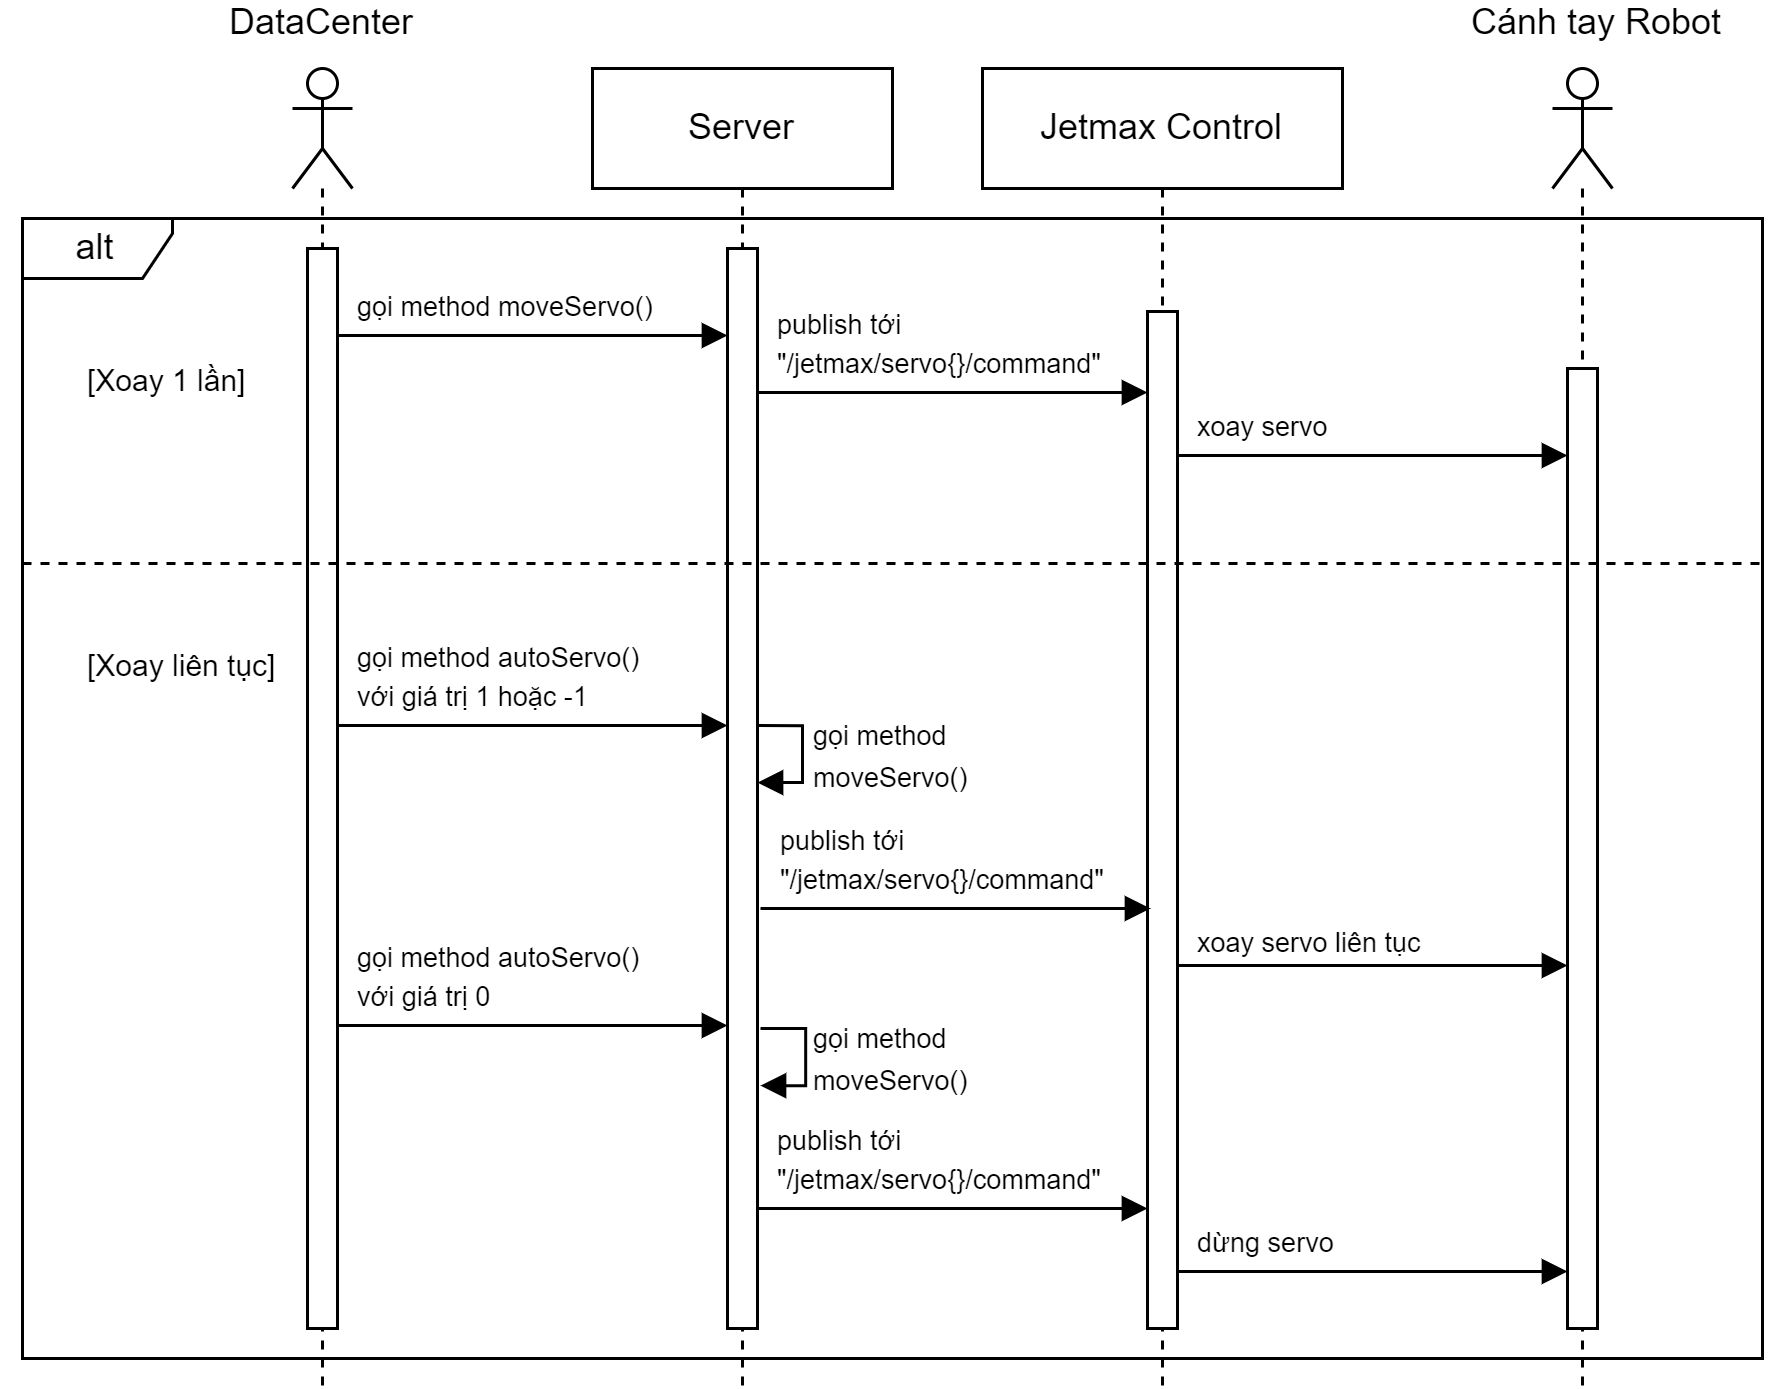
\includegraphics[width=0.8\textwidth]{Images/Implementation/Control/dieukhientheo_servo.jpg}
        \caption{Sequence diagram của điều khiển theo servo}
    \end{figure}

    
    
    \item \textbf{Điều khiển cánh tay theo tọa độ:} Tương tự như điều khiển bằng servo thì ở tính năng này method mà Server cung cấp có tên là \textbf{moveCordinate}, Server sẽ publish vào topic ROS có tên là "/jetmax/relative\_command" với tham số truyền vào là một message chứa ba tọa dộ x, y, z. Bên dưới Jetmax Control thực thi bằng cách lấy tọa độ hiện tại và cộng vào tọa độ được truyền vào (relative). Dưới đây là sequence diagram của chức năng này:
    \begin{figure}[!h]
        \centering
        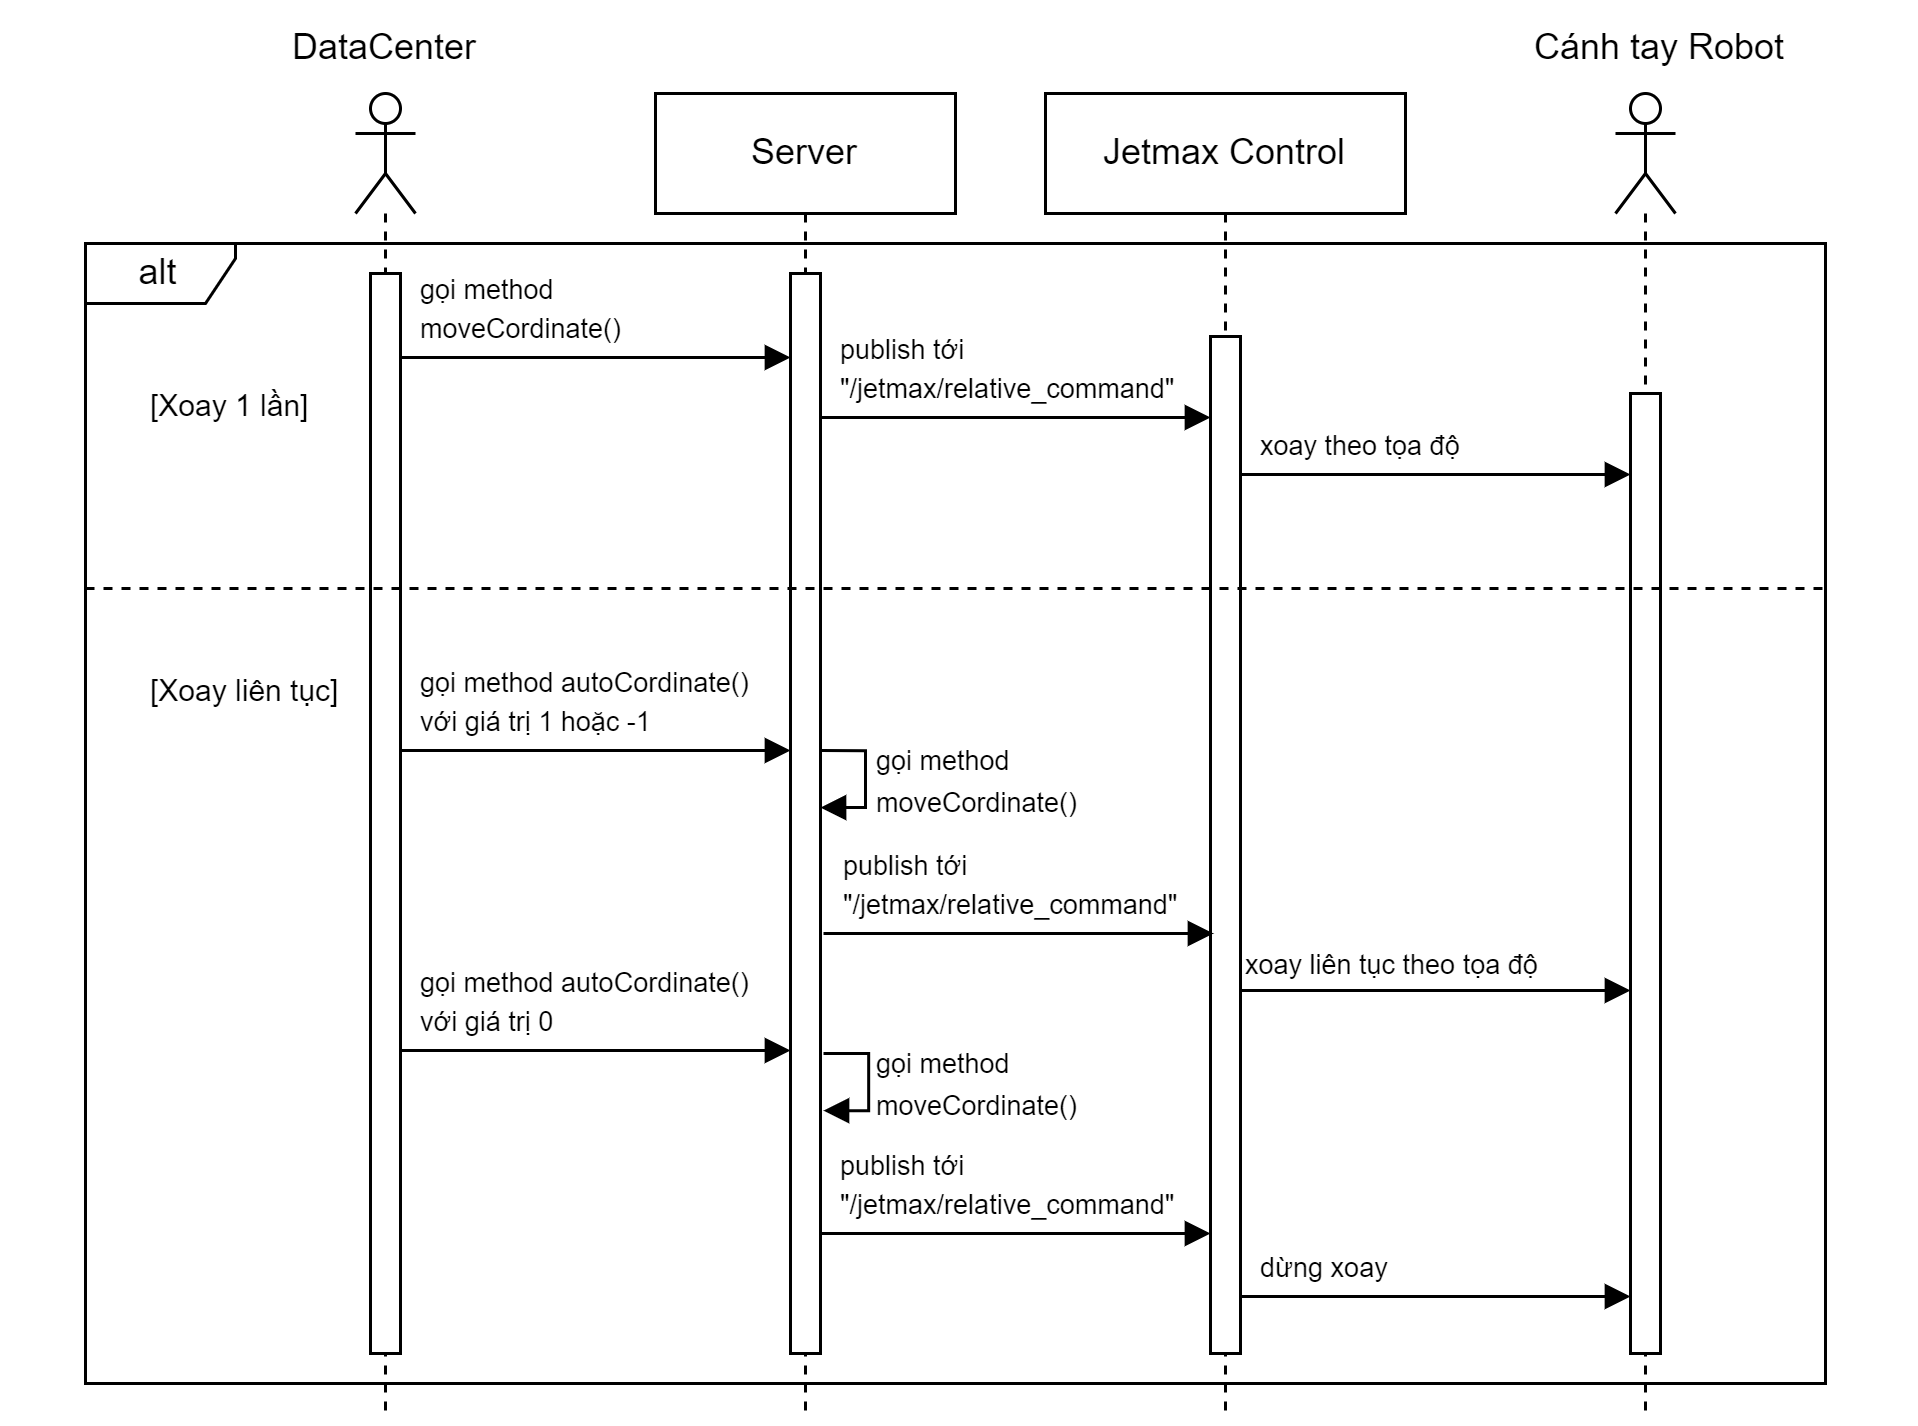
\includegraphics[width=0.8\textwidth]{Images/Implementation/Control/dieukhientheo_toado.jpg}
        \caption{Sequence diagram của điều khiển theo tọa độ}
    \end{figure}

    \newpage
    
    \item \textbf{Thay đổi tốc độ xoay:} Để thay đổi tốc độ xoay của các servo, Server OPC cung cấp method có tên là \textbf{changeSpeed}, khi method được gọi, phía Server sẽ lưu tốc độ này vào 1 biến toàn cục. Biến này sẽ được đính kèm vào các message khi gọi tới các topic ROS kiểm soát chuyển động cánh tay. Bên dưới là sequence diagram của chức năng:
    \begin{figure}[!h]
        \centering
        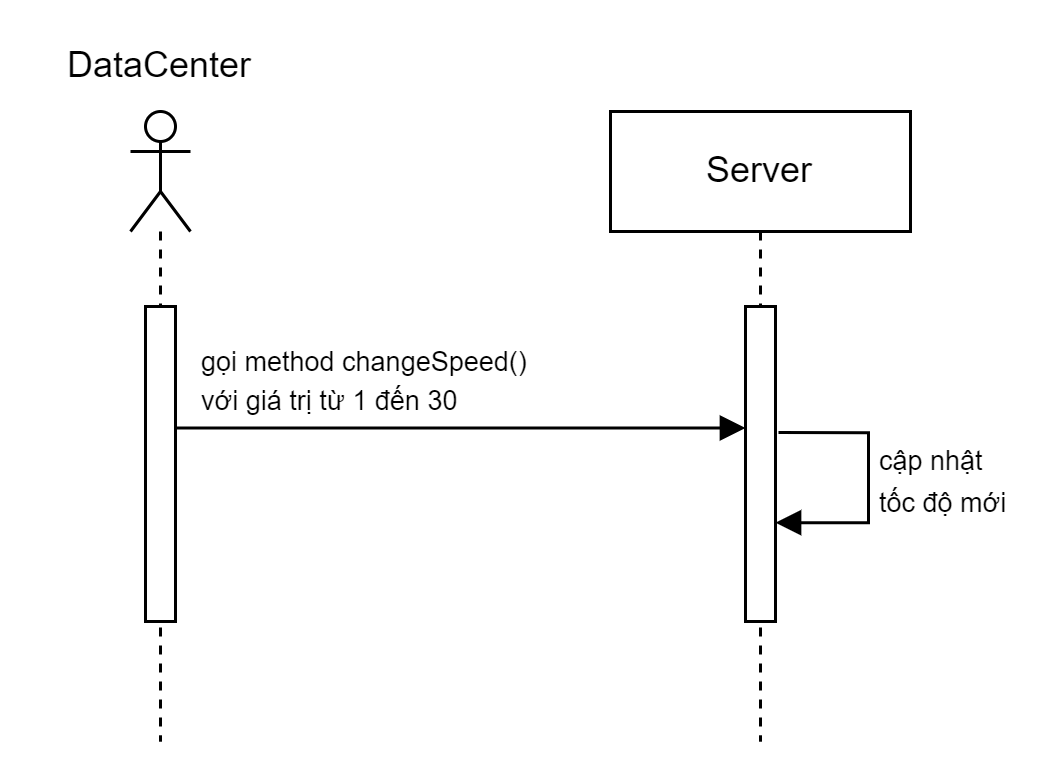
\includegraphics[width=0.6\textwidth]{Images/Implementation/Control/changespeed.jpg}
        \caption{Sequence diagram của thay đổi tốc độ xoay}
    \end{figure}
    
    \item \textbf{Về vị trí ban đầu:} Đây là chức năng đưa cánh tay về 1 vị trí mặc định đã được chọn trước, ở vị trí này cánh tay sẽ có tọa độ là \{x = 0,y = -162.9, z = 212.8\} và gốc các servo mid=500,left=500,right=500, các giá trị khác tương ứng gripper=90, rotator=90. Method này có tên là \textbf{goHome}; khi gọi tới method, Server sẽ thực thi việc gọi tới service ở topic ROS có tên là "/jetmax/go\_home" với một message rỗng ( Empty ). Dưới đây là sequence diagram cho chức năng:
    \begin{figure}[!h]
        \centering
        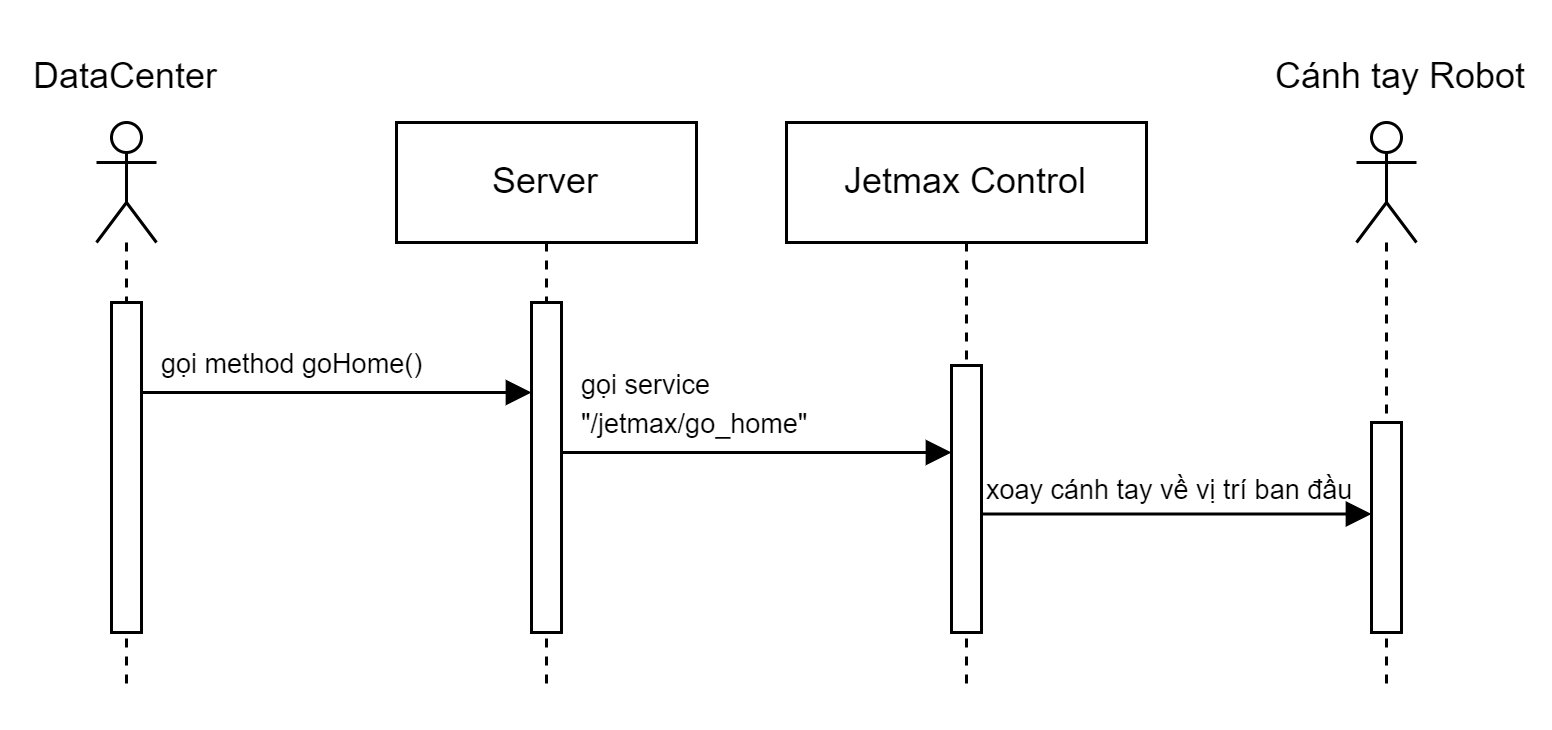
\includegraphics[width=0.8\textwidth]{Images/Implementation/Control/goHome.jpg}
        \caption{Sequence diagram của về vị trí ban đầu}
    \end{figure}
    
    \item \textbf{Bật tắt sucker:} Để bật hoặc tắt máy hút được gắn ở đầu của cánh tay, Server cung cấp một method có tên là \textbf{sucker}. Khi được gọi Server sẽ thực hiện publish một message có giá trị là TRUE hoặc FALSE vào topic ROS có tên "/jetmax/end\_effector/sucker/command". Dưới đây là sequence diagram của chức năng:
    \begin{figure}[!h]
        \centering
        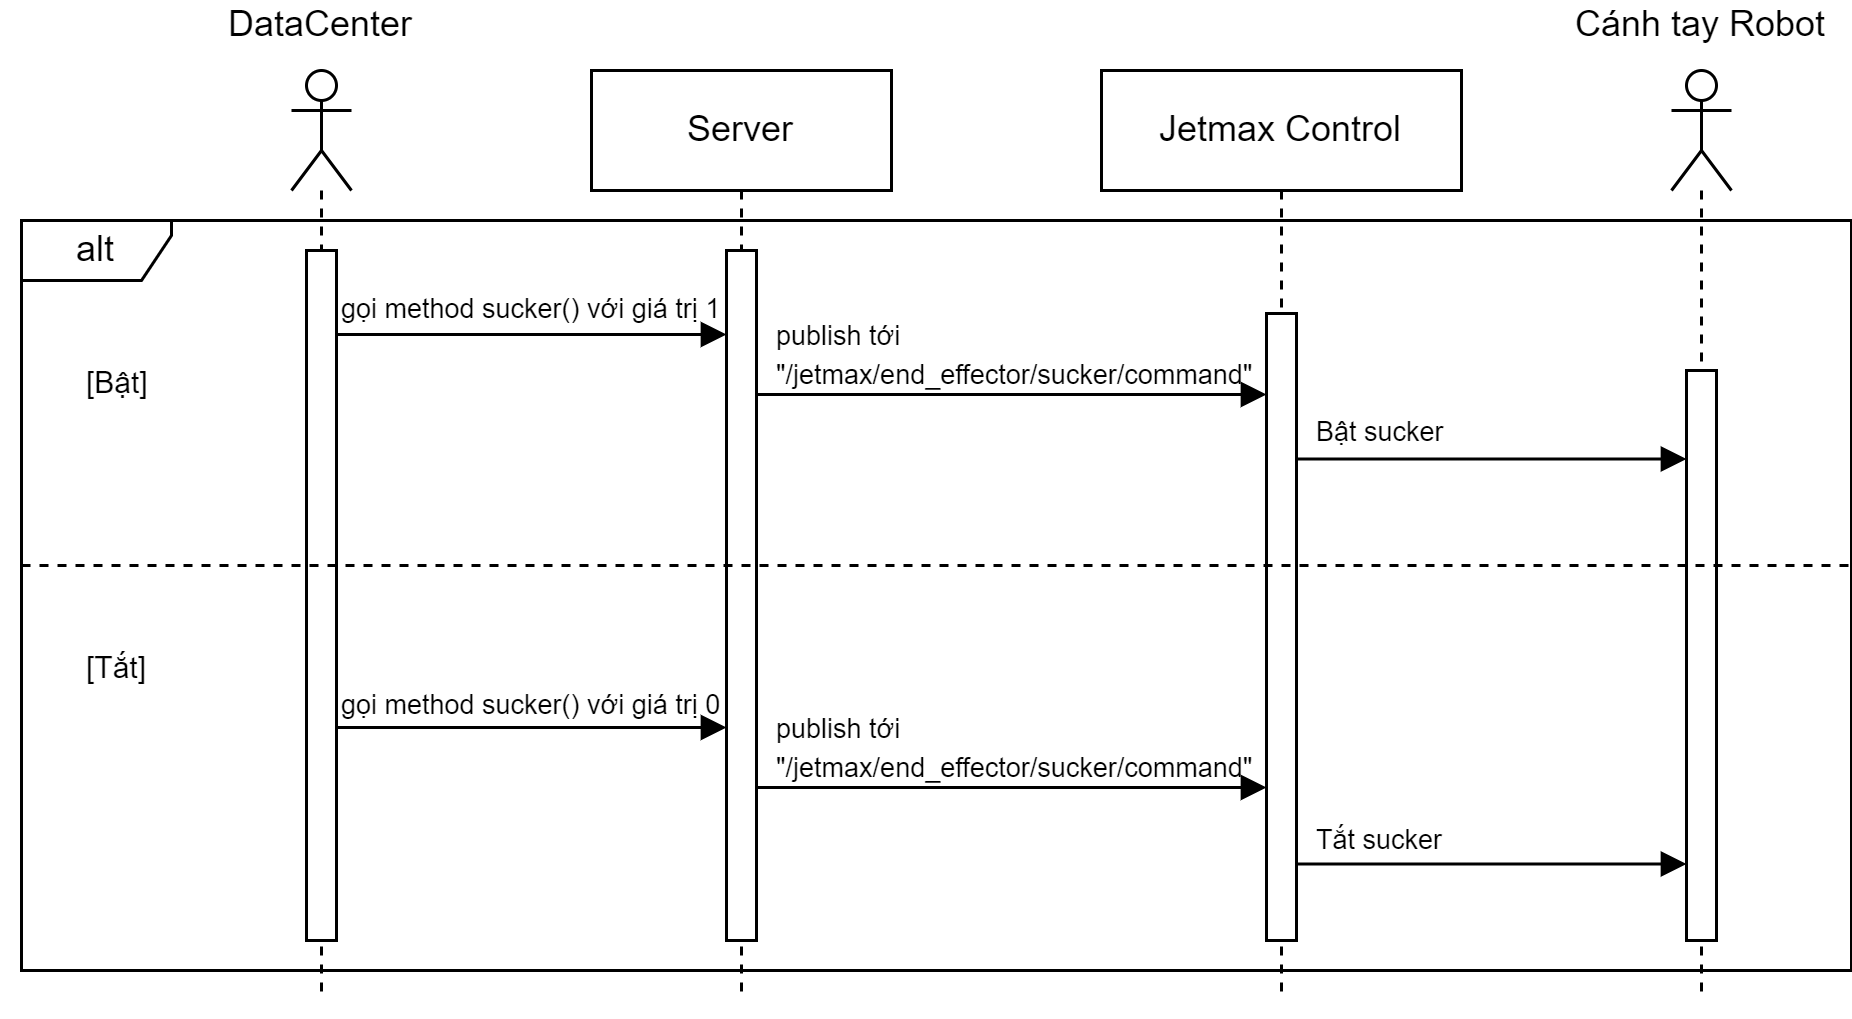
\includegraphics[width=0.8\textwidth]{Images/Implementation/Control/sucker.jpg}
        \caption{Sequence diagram của bật tắt sucker}
    \end{figure}
    
    \item \textbf{Đưa cánh tay tới tọa độ:} Khác với chức năng điều khiển theo servo, ở chức năng này cánh tay sẽ di chuyển tới một vị trí nhất định thay vì dùng lại tọa độ cũ cộng vào tham số. Server cung cấp method \textbf{setCordinate} để thực hiện chức năng này, khi được gọi Server sẽ thực hiện publish 1 message chứa tọa độ \{x, y, z\} vào topic ROS "/jetmax/command", khi nhận được tín hiệu cánh tay sẽ lập tức di chuyển đến toạ độ mới có giá trị là \{x, y, z\}. Bên dưới là sequence diagram của chức năng:
    \begin{figure}[!h]
        \centering
        \includegraphics[width=0.8\textwidth]{Images/Implementation/Control/setCordinate.jpg}
        \caption{Sequence diagram của đưa cánh tay tới tọa độ}
    \end{figure}
    
    \item \textbf{Kich hoạt AI xếp gỗ:} Cánh tay jetmax được tích hợp một số dịch vụ AI kèm theo, trong đó tiêu biểu là chức năng sắp xếp các khối gỗ theo thứ tự và theo dõi vật thể với màu sắc cụ thể. Để kích hoạt tính năng sắp xếp khối gỗ, bước đầu tiên chúng ta gọi tới method có tên \textbf{AIservice} được cung cấp trong Server OPC, truyền vào đó tên của chức năng và tham số thứ 2 là một biên boolean với giá trị TRUE nếu kich hoạt hoặc FALSE để thoát khỏi chức năng này. Khi method được gọi Server dựa vào giá trị được gửi đến, sau đó thực hiện gọi tới một service với topic ROS có tên là "/\{service\_name\}/enter"; ở đây service\_name là tên của dịch vụ AI tức "palletizing". Tiếp theo để AI chạy, chúng ta cần gọi tới method \textbf{AIserviceRun} truyền vào đó tên của dịch vụ ở đây chúng ta sử dụng "palletizing", Server sẽ tiếp tục thực hiện gọi 1 service khác có tên là "/\{service\_name\}/set\_running". Sau đó AI sẽ hoạt động cánh tay sẽ tìm và sắp xếp các khối gỗ theo thứ tự của id. Để thoát khỏi AI này ta gọi tới method ban đầu và truyền vào đó giá trị FALSE. Bên dưới là sequence diagram của chức năng kích hoạt/thoát AI xếp gỗ.
    \begin{figure}[!h]
        \centering
        \includegraphics[width=0.8\textwidth]{Images/Implementation/Control/palletizing.jpg}
        \caption{Sequence diagram của kích hoạt AI xếp gỗ}
    \end{figure}

    \newpage
    
    \item \textbf{Kich hoạt AI theo dõi màu:}AI này được phát triển trên thư viện OpenCV, dùng trong việc nhận diện màu sắc của khối vật thể. Tương tự như sắp xếp khối gỗ, để kích hoạt theo dỗi khối màu lần lượt gọi tới các method sau:
    \begin{itemize}
        \item \textbf{AIservice}: Để kích hoạt AI với tên truyền vào là "object\_tracking",giá trị boolen kèm theo là TRUE.
        \item \textbf{AIsetTarget}: Tiếp theo để set màu của khối object cần theo dõi, ta gọi method này với giá trị truyền vào là tên của AI "object\_tracking", màu tương ứng "red", "green", hoặc "blue".
        \item \textbf{AIserviceRun}: Cuối cùng để AI hoạt động thì phải gọi tới method này với các giá trị tương ứng.
    \end{itemize}
    Để thoát khỏi AI ta gọi tới \textbf{AIservice} với giá trị boolen là FALSE để thoát. Sau đây là sequence diagram cho chức năng này.
    \begin{figure}[!h]
        \centering
        \includegraphics[width=0.8\textwidth]{Images/Implementation/Control/object-tracking.jpg}
        \caption{Sequence diagram của kích hoạt AI theo dõi màu}
    \end{figure}

    \newpage
    
    \item \textbf{Kich hoạt AI phân loại rác:} Đây là tính năng mà nhóm đã phát triển, là sự kết hợp của các bài toán như: nhận diện màu bằng OpenCV, nhận diện vật thể thông qua kỹ thuật học có giám sát (supervised learning) được thực hiện trên mô hình YOLOv5. Cụ thể sẽ được trình bày ở phần sau.Để kích hoạt AI này, cần thực hiện gọi tới các method sau Server:
    \begin{itemize}
        \item \textbf{AIservice:} Gọi tới method này với giá trị truyền vào là "waste\_classification" và giá trị boolean kèm theo là TRUE.
        \item  \textbf{waste\_class:} Gọi tới method này để thiết lập loại rác mong muốn.

        \item  \textbf{AIserviceRun}: Để AI được khởi chạy, gọi method này với các tham số tương ứng.
        
        \item  \textbf{set\_suck\_waste}:Khi AI đã hoạt động, gọi method này với tham số truyền vào là các giá trị từ 1 đến 4, tương ứng cho các trạng thái của chức năng "tìm và gắp", "tìm và thả".     
    \end{itemize}
    Để thoát khỏi AI ta gọi tới \textbf{AIservice} với giá trị boolen là FALSE để thoát. Sau đây là sequence diagram cho chức năng này.
    \begin{figure}[!h]
        \centering
        \includegraphics[width=0.8\textwidth]{Images/Implementation/Control/waste-classification.jpg}
        \caption{Sequence diagram của kích hoạt AI phân loại rác}
    \end{figure}

    \newpage
    
    \item \textbf{Cập nhật trạng thái cánh tay:} Server sẽ luôn lắng nghe các giá trị trạng thái của canh tay thông qua các topic ROS mà khối Jetmax Control tạo ra, sau đó cập nhật liên tục các giá trị này lên các node, cung cấp cho người dùng trạng thái theo thời gian thực của thiết bị - cụ thể là cánh tay Jetmax. Các topic ROS được Server OPC lắng nghe gồm:
    \begin{itemize}
        \item \textbf{/jetmax/status:} Lây trạng thái tọa độ, góc servo của cánh tay, trạng thái đầu hút...
        \item  \textbf{/jetmax/AIEnterCurrent, /jetmax/AIRunCurrent, /jetmax/AIColorCurrent}: Lấy thông tin của chức năng AI hiện tại đang hoạt động trên cánh tay.
        \item \textbf{/waste\_classification/set\_suck, /waste\_classification/\\
        set\_waste\_class:} Lây thông tin chi tiết của AI phân loại rác.
        \item \textbf{/usb\_cam/image\_rect\_color:} Lấy dữ liệu hình ảnh mặc định từ usb camera tích hợp trên cánh tay Jetmax. 
        \item \textbf{/{topic}/image\_result:} Lấy dữ liệu ảnh đã được xử lý trong các chức năng AI khi các chức năng AI này được kích hoạt. Dữ liệu hình ảnh sẽ được lấy từ topic này thay vì topic mặc định usb\_cam
    \end{itemize}
    Những dữ liệu này sau khi lắng nghe sẽ được cập nhật vào các node tương ứng trên Server OPC. Ngoài ra, nhóm cũng thực hiện gửi dữ liệu ảnh thu được từ camera lên node OPC UA của Server. Tuy nhiên, vì dữ liệu ảnh khá lớn (kích thước 640 * 480 * 3 = 921600 byte cho từng tấm ảnh),Server OPC UA không thể xử lý và gửi toàn bộ lượng dữ liệu đó với tốc độ nhanh, liên tục. Chính vì thế, riêng đối với dữ liệu ảnh, nhóm đã phải sử dụng giải thuật nén của thư viện PIL (Python Imaging Library) và thư viện OpenCV để nén ảnh lại xuống còn khoảng 8900 bytes, đánh đổi giảm bớt kích thước ảnh và chất lượng ảnh nhằm tăng khả năng đáp ứng của Server. Dưới đây là sequence diagram cho chức năng này: 
    \begin{figure}[!h]
        \centering
        \includegraphics[width=0.8\textwidth]{Images/Implementation/Control/update-state.jpg}
        \caption{Sequence diagram của cập nhật trang thái cánh tay}
    \end{figure}
\end{itemize}


\newpage

\section{Tính năng AI: Phân loại rác thải bán tự động}

Một trong những vấn đề lớn nhất của thế giới hiện nay là ô nhiễm môi trường. Nhiều nỗ lực đã được thực hiện để giảm thiểu ô nhiễm, và trong đó việc phân loại rác đóng vai trò quan trọng. Tuy nhiên, phân loại rác thủ công có thể là một quá trình phức tạp và tốn thời gian. Để giải quyết vấn đề này, công nghệ trí tuệ nhân tạo (AI) đã được sử dụng để xây dựng các hệ thống phân loại rác tự động. Trong đồ án này, nhóm đã thiết kế và hiện thực chức năng phân loại rác bán tự động dựa trên AI, với hy vọng đóng góp một phần nhỏ vào việc giảm thiểu ô nhiễm môi trường.

Tính năng phân loại rác thải đã và đang được nghiên cứu trong khá nhiều bài báo. Vào năm 2016, Williams và Bentil \cite{williams2016design} giới thiệu và hiện thực một hệ thống tự động sắp xếp rác thải sử dụng vi điều khiển, và đã thành công phân loại rác thải hữu cơ và rác thải vô cơ sử dụng cảm biến khí gas. Paulraj \cite{gundupalli2016automated} đề xuất giải thuật để nhận biết rác thải trên hình ảnh chụp được từ camera nhiệt. Tác giả cũng xây dựng một cánh tay robot 5 bậc tự do tích hợp camera nhiệt, cảm biến khoảng cách để thực hiện phân loại rác. Sadia Zahin Diya \cite{diya2018developing} trong nghiên cứu vào năm 2018, xây dựng một hệ thống phân loại rác thải thông minh với mục tiêu phù hợp trong bối cảnh quốc gia Bangladesh. Trong nghiên cứu của mình, tác giả xây dựng hệ thống điều khiển và phân loại rác có khả năng nhận biết rác thải kim loại, hữu cơ và nhựa sử dụng các cảm biến IR (Infrared Ray), cảm biến từ trường và cảm biến hiệu điện thế. Các nghiên cứu đều thử nghiệm với rác thải thực tế, tuy nhiên chỉ có thể phân loại một số loại rác cố định.


Về phía nhóm, việc thực hiện tính năng AI phân loại rác không phải là mục tiêu chính của đề tài, nhưng đây là một chức năng sáng giá để thể hiện khả năng điều khiển thiết bị thông qua OPC UA. Nhà phát triển cánh tay JetMax - Hiwonder đã cung cấp sẵn cho cánh tay robot chức năng phân loại rác tự động, tuy nhiên không phải là rác thực tế mà chỉ là ảnh các rác thải được in lên một tấm thẻ hình vuông. Các rác thải buộc phải đặt ngay phía trước cánh tay khi cánh tay ở vị trí mặc định để nhận dạng, và khi nhận diện được rác thải, sẽ tự động mang rác tới một vị trí được chỉ định. Vì những giới hạn này, nhóm quyết định nâng cấp tính năng phân loại rác này thành "phân loại rác bán tự động" hoạt động theo máy trạng thái. Về khái niệm "bán tự động", khi này nhóm có thể tự do đặt rác thải ở một nơi khác và điều khiển cánh tay thủ công tới để tự động hút lên bằng AI. Sau khi hút, nhóm lại điều khiển cánh tay thủ công tới khu vực thùng rác, và để cánh tay tự nhận diện loại thùng rác cần bỏ rác vào. Việc nhận diện rác thải và thùng rác được thực hiện bằng cách phân tích ảnh chụp từ USB camera và các thuật toán AI đã được huấn luyện sẵn có trong cánh tay JetMax. Vì giới hạn về thời gian và điều kiện, nhóm vẫn thực hiện nhận dạng rác thải dưới dạng các thẻ vuông để dễ dàng hút bằng đầu hút của cánh tay JetMax.

\subsection{Yêu cầu hệ thống}

Phần tiếp theo, nhóm đề ra một số yêu cầu chức năng và phi chức năng cho tính năng AI phân loại rác thải, để làm rõ hoạt động mong đợi và khả năng của tính năng này.

\subsubsection{Yêu cầu phi chức năng}


Các yêu cầu phi chức năng cho tính năng này được nhóm đặt ra như sau:
\begin{itemize}
    \item Chức nằng này phải đảm bảo độ chính xác và đáng tin cậy trong việc phân loại các loại rác khác nhau, từ đó giúp người dùng phân biệt dễ dàng và đúng đắn.
    \item Hệ thống phân loại rác cần được thiết kế để có thể mở rộng trong tương lai, khi có thêm các loại rác mới cần phân loại.
    \item Tính năng phân loại rác cần được thiết kế để tương tác dễ dàng và trực quan với người dùng, giúp họ sử dụng một cách thuận tiện và hiệu quả.
    \item Độ trễ phản hồi của tính năng không quá 1 giây
\end{itemize}
\subsubsection{Yêu cầu chức năng}
Các yêu cầu về chức năng cho tính năng phân rác bán tự động như sau:
\begin{itemize}
    \item Nhận diện được loại rác cụ thể và xác định được vị trí của nó.
    \item Nhận diện được loại thùng rác tương ứng với từng loại rác và vị trí của nó
    \item Người dùng có thể điều khiển qua lại để đưa camera bắt được hình ảnh của rác hoặc thùng rác.
    \item Xác định vùng hoạt động tốt cho camera
    \item Thao tác hút hoặc thả trên cùng một phím nhấn.
\end{itemize}
\subsection{Sơ đồ use case diagram}
Dựa vào những yêu cầu phi chức năng và chức năng mà nhóm xem xét bên trên, nhóm đưa ra một use case đơn giản cho chức năng Phân loại rác bán tự động như hình.

    \begin{figure}[!h]
        \centering
        \includegraphics[width=0.8\textwidth]{Images/Implementation/AI/waste_usecase.jpg}
        \caption{Use case diagram của phân loại rác bán tự động}
    \end{figure}



Người dùng sẽ tương tác với chức năng phân loại rác bán tự động này bằng VR app được nhóm phát triển trên Unity3D và chạy trên Oculus, ứng dụng gửi nhận dữ liệu từ cánh tay thông qua module trung gian Datacenter, sẽ được giới thiệu ở phần tiếp theo. Cánh tay và chức năng AI sẽ được quản lý bởi máy tính nhúng Jetson Nano chứa một server OPC trên đó.
\subsection{Hiện thực chức năng phân loại rác bán tự động}
Chức năng được nhóm hiện thực dựa trên hai thư viện nổi tiếng là OpenCV và YOLOv5, trong chức năng này nhóm chia ra làm hai chức năng nhỏ cần hiện thực.

\begin{itemize}
    \item Thứ nhất, nhóm sử dụng kỹ thuật học có giám sát ( supervise learning ) để train cho mô hình AI nhận diện các loại rác. Ở chức năng này nhóm sử dụng thư viện YOLOv5 trên python để train data cho mô hình. Khi camera dò được thẻ rác nào đó, mô hình sẽ trả về các thông tin như tên rác, loại rác và vị trí của vật thể so với đầu hút. Từ những thông tin đó, AI sẽ tính toán và đưa ra vị trị tương ứng để đưa đầu hút của cánh tay tới vị trí của mảnh rác và hút nó.
    \item Thứ hai, nhóm sử dụng chức năng nhận diện màu sắc được tích hợp trong thư viện OpenCV để nhận diện những loại thùng rác. Sau khi hút rác, người dùng sẽ di chuyển cánh tay sao cho camera nhìn thấy các thùng rác, AI sẽ tự động chọn thùng phù hợp với loại rác hiện tại và thả và đó. Cũng tương tự như quá trình tìm và nhận diện rác, quá trình nhận diện loại thùng rác cũng sẽ trả về các thông tin như loại rác, vị trí của thùng đó so với đầu hút. Dựa vào đó ta sẽ tìm được vị trí so với cánh tay và thả rác vào đó.
\end{itemize}

Chức năng sẽ có 4 trạng thái chính, được mô tả như sau:
    \begin{figure}[!h]
        \centering
        \includegraphics[width=0.8\textwidth]{Images/Implementation/AI/state-machine_1.jpg}
        \caption{Sơ đồ máy trạng thái của chức năng}
    \end{figure}
\begin{itemize}
    \item \textbf{IDLE:} Đây là trạng thái đầu tiên khi chức năng được khởi động, ở trạng thái này camera sẽ cung cấp hình ảnh cho AI nhận diện rác thải và đợi một event trigger từ người dùng, nếu phát hiện được rác thuộc loại cần phân loại, AI sẽ vẽ một khung hình chữ nhật bao quanh loại rác đó và kèm theo nhãn của loại rác. Khi nhận event trigger từ người dùng chức năng chuyển sang trạng thái thứ 2 SUCK.
    \item \textbf{SUCK:} Ở trạng thái AI sẽ cung cấp vị trí của vật thể gần nhất so với camera, để di chuyển chính xác ta cần vị trí của vật thẻ so với cánh tay, vị trị này sẽ có được sau khi qua một vài bước tính toán và sẽ được trình bày trong phần tiếp theo. Sau khi tính được vị trí cần đến, cánh tay sẽ di chuyển, hút vật thể, đi lên theo chiều Z và chuyển sang trạng thái HOLD.
    \item  \textbf{HOLD:} Ở trạng thái này, camera sẽ nhận diện thùng rác dựa vào màu sắc được thiết lập trước đó, tương ưng cho từng loại rác, ở trạng thái này người dùng sẽ di chuyển cánh tay qua lại để tìm được vị trí của thùng rác, khi xác định được vị trí và nhận event trigger sẽ chuyển sang trạng thái tiếp theo RELEASE.
    \item \textbf{RELEASE:} Khi xác định được vị trí của thùng rác so với camra, cũng tương tự sẽ tinh toán như ở trạng thái SUCK, tìm ra vị trị so với cánh tay, cánh tay sẽ di chuyển đến thả vật thể và quay về trạng thái IDLE.
\end{itemize}
\subsubsection{Xác định vị trí của vật thể so với cánh tay}
Ở hai trạng thái \textbf{SUCK} và \textbf{RELEASE}, các mô hình AI trả về cho ta một tọa độ vị trí của vật thể gần nhất, tuy nhiên đây là tọa độ của vật thể so với camera, để cánh tay đến được vật thể thì phải qua một bước tính toán, chuyển từ tọa độ so với camera thành tọa độ so với cánh tay.
\begin{figure}[!h]
    \centering
    \includegraphics[width=0.6\textwidth]{Images/Implementation/AI/AI_math_1.jpg}
    \caption{Mô tả bài toán}
\end{figure}

Trong hình bên trên O là góc tọa độ cánh tay, O' là gốc tọa độ của camera, AI sẽ cung cấp cho ta tọa độ vật thể A trong tọa độ x'O'y', chúng ta cần chuyên tọa độ này thành tọa độ mời trong hệ xOy. Nhóm giải quyết qua hai bước sau:
\begin{itemize}
    \item Tìm góc tạo bởi vật thể A (OA) và trục Oy của cánh tay, sau đó xoay servo mid theo góc tìm được lúc ta có O, O', A thẳng hàng. Sau đó chuyển sang bước tiếp theo.
    
    \begin{figure}[!h]
        \centering
        \includegraphics[width=0.6\textwidth]{Images/Implementation/AI/AI_math_2.jpg}
        \caption{Sau khi xoay cánh tay theo gốc alpha}
    \end{figure}

    \item  Công thức tính gốc xoay \[\angle alpha = arctan( \frac{x'}{OO'+y'} ) \] 
     
    \item Sau khi xoay servo mid của cánh tay theo góc tìm được ở bước một, ta có O, O', A thẳng hàng, tìm được độ dài của OA, OO' và có được tọa độ điểm O' trong xOy, dựa vào biểu thức vector: OA = alpha*OO', trong đó ta tìm được alpha theo biểu thức độ dài, từ đó ta suy ra được tọa độ điểm A trong hệ tọa độ xOy.
\end{itemize}

Sau khi tìm được vị trí điểm A cánh tay sẽ di chuyển tới tọa độ đó và thực hiện thao tác hút/thả với vật thể.

\subsubsection{Sequence diagram của chức năng}

Trong phần tiếp theo sau đây, nhóm sẽ trình bày cụ thể hơn về sơ đồ mô tả cách thức hoạt động của chức năng.

\begin{figure}[!h]
    \centering
    \includegraphics[width=0.9\textwidth]{Images/Implementation/AI/AI-sequence.png}
    \caption{Sequence diagram của chức năng}
\end{figure}

Quan sát sequence diagram, ta có thể nói chi tiết hoạt động của chức năng như sau:
\begin{itemize}
    \item Khi AI được khởi động, chương trình sẽ thiết lập loại rác tương ứng mà người dùng nhập vào, lúc này chức năng sẽ nằm ở trạng thái IDLE, ở trạng thái này camera sẽ nhận diện được những mãnh rác thuộc loại rác mà người dùng đã thiết lập, hình ảnh cùng các trạng thái sẽ liên tục được cập nhật vào OPC server thông qua các node của ROS.
    Lúc này người dùng sẽ xoay các servo để đưa các mãnh rác vào vùng nhận diện của camera.
    \item Sau khi nhận diện và phát hiện vật thể tương ứng, người dùng sẽ kích hoạt một event gắp rác, lúc này trạng thái của chức năng sẽ chuyển sang SUCK, ở trạng thái này, AI sẽ tính toán lại tọa độ, đưa đầu hút đến tọa độ đó và hút, sau khi hút xong cánh tay sẽ di chuyển lên trên và chuyển sang trạng thái HOLD, trong quá trình này, người dùng không cần thao tác vào cánh tay cho đên khi cánh tay dừng lại và chờ event tiếp theo được kích hoạt
    \item Ở trạng thái HOLD người dùng sẽ di chuyển cánh tay đưa thùng rác tương ứng vào vùng nhận diện của camera, lúc này camera sẽ nhận diện thùng rác theo màu tương ứng với loại ra mà người dùng thiết lập, người dùng sẽ xoay cánh tay để đưa thùng rác vào vùng nhận diện của camera để tiến hành phân loại.
    \item  Khi nhận diện được thùng rác, người dùng kích hoạt một event để thả rác vào thùng, khi event được kích hoạt, chức năng sẽ chuyển sang trạng thái RELEASE, ở trạng thái này AI sẽ tính toán lại tọa độ, đưa cánh tay đến tọa độ mới và thả vật thể đang hút ra. Sau khi thả cánh tay sẽ di chuyển lên trên và chuyển sang trạng thái ban đầu tức IDLE, trong quá trình này, người dùng không cần thao tác vào cánh tay cho đến khi cánh tay dừng lại và chờ event tiếp theo được kích hoạt.
\end{itemize}
 
\section{Module Datacenter}
% mô tả về datacenter

% Như đã trình bày ở phần kiến trúc hệ thống tổng quát, Datacenter là một module trung gian giữa module Control và module VR application. Sự kết hợp của Datacenter giúp cho ta có thể mở rộng mô hình điều khiển trong tương lai, khi có thể kết nối nhiều OPC server hơn vào Datacenter, để Datacenter tổng hợp dữ liệu, và sau đó ứng dụng VR có thể truy cập vào 1 điểm duy nhất là Datacenter để thực hiện điều khiển nhiều thiết bị một cách tiện lợi.

% Hiện tại, do giới hạn về tài nguyên và thiết bị, Datacenter chỉ đang kết nối với 1 OPC server của \textbf{module Control} nhằm điều khiển cánh tay. Khi chạy module Datacenter, nó sẽ tiến hành tạo kết nối với server OPC chạy trong module Control, sau đó "sao chép" - tạo ra những node và method bản sao lên Datacenter. 

Datacenter, hay có thể hiểu là một module với vai trò tập trung dữ liệu vào một điểm duy nhất nhằm xử lý, đồng bộ hoặc trở thành một gateway cho liên kết với cloud server hoặc ứng dụng từ xa. Việc sử dụng một module tập trung dữ liệu cũng giảm bớt độ phức tạp giữa các kết nối và giao tiếp, đặc trưng là khi người dùng chỉ cần kết nối tới module này là đủ để thu thập toàn bộ thông tin cần biết mà không cần phải đào sâu vào từng vị trí cụ thể. Đối với OPC UA, kể từ khi ra mắt, đã có nhiều nghiên cứu nhằm đề xuất một kiến trúc mang tính mở rộng dành cho OPC UA, hỗ trợ thu thập dữ liệu từ nhiều OPC UA server tại một nơi thay vì kiến trúc 1 client - 1 server mặc định. Fembach \cite{fernbach2014opc} giới thiệu một kiến trúc đa tác nhân (multi-agent) trong nghiên cứu gồm hai lớp OPC UA server. Lớp đầu tiên gồm 2 OPC UA server được cài đặt ở hai vị trí khác nhau để quan sát dữ liệu, và cả hai server này đều báo cáo dữ liệu tới một server OPC UA tổng hợp trên lớp thứ hai thông qua mạng không dây. Haskamp \cite{haskamp2018implementing} giới thiệu một kiến trúc khác nhằm nâng cấp các PLC truyền thống trở nên phù hợp với nền công nghiệp 4.0 tận dụng giao thức OPC UA. Các PLC chạy OPC server đều sẽ gửi dữ liệu lên dataFEED OPC Suite - một OPC UA server trung gian. Dữ liệu gửi lên đây cũng được dùng để gửi lên dịch vụ đám mây Microsoft Azure, từ đó có thể truy xuất, thu thâp bởi các ứng dụng quan trắc, điều khiển từ xa khác. Ahmad Abdelsattar \cite{abdelsattaropcgateway} đề xuất một khối gọi là Client/Gateway Node, gồm một OPC UA client có nhiệm vụ trung tâm thu thập thông tin từ các OPC server khác chạy trên PLC hoặc máy tính nhúng, nhằm cung cấp dữ liệu cho các ứng dụng nội bộ như Digital Twin, SCADA, hơn nữa cũng trở thành một gateway để giao tiếp với các dịch vụ đám mây thông qua các giao thức thông dụng TCP/IP hoặc UDP.


Trong đồ án này, nhóm cũng hiện thực kiến trúc với khối Datacenter - một module trung gian để tập trung dữ liệu nhằm giảm bớt sự phức tạp về hệ thống kết nối, vừa tạo khả năng mở rộng của hệ thống sau này. Trên Datacenter này sẽ có thể có nhiều OPC UA client, mỗi một client đảm nhiệm việc kết nối tới từng OPC UA server cần thu thập thông tin. Sau đó, các OPC UA client này sẽ cung cấp thông tin và dữ liệu cần thiết cho một OPC UA server chính chạy trên Datacenter, đóng vai trò trở thành điểm truy cập tập trung cho ứng dụng cần tiêu thụ dữ liệu. Hiện tại, hiện thực của nhóm chỉ bao gồm một OPC UA client để kết nối với OPC UA server bên module Control, và một OPC UA server chính trên Datacenter với khả năng tạo ra bản sao các node và method, cấu trúc dữ liệu giống hệt OPC server của module Control, đồng thời cập nhật liên tục theo thay đổi của module Control. Datacenter giờ trở thành khối tập trung và trung gian của dòng dữ liệu giữa ứng dụng và thiết bị thật.


% requirement
\subsection{Yêu cầu hệ thống}

Trước khi tiến hành hiện thực module Datacenter, ta cần đề ra những yêu cầu dành cho module này, về mặt phi chức năng và chức năng.

\subsubsection{Yêu cầu phi chức năng}

Các yêu cầu phi chức năng dành cho module Datacenter được đề ra:


\begin{itemize}
    \item Datacenter phải được thiết kế để độc lập với sự phát triển của module Control - Sự thay đổi của module Control gây ảnh hưởng ít hoặc không ảnh hưởng tới hiện thực của Datacenter
    \item Độ trễ cập nhật giá trị node trên Datacenter khi có sự thay đổi ở module Control không quá 1 giây
    \item Datacenter phải chịu được lượng kết nối vào lớn
    \item Datacenter được hiện thực có khả năng mở rộng thêm số lượng server OPC kết nối tới.
    \item Datacenter có khả năng hồi phục trong trường hợp mất kết nối tạm thời với server.
\end{itemize}

\subsubsection{Yêu cầu chức năng}

Các yêu cầu chức năng dành cho module Datacenter được đề ra:

\begin{itemize}
    \item Datacenter có thể browse các node trên OPC server được kết nối tới
    \item Datacenter có các variable node tự động cập nhật theo sự thay đổi của variable của server
    \item Datacenter tạo ra các method "bọc" gọi method tới server
    \item Datacenter cho phép người dùng tương tác với các node bằng cách kết nối tới OPC server đang chạy trong Datacenter.
    \item Datacenter sử dụng mã hóa dữ liệu 
\end{itemize}

% usecase
\subsection{Sơ đồ use case và máy trạng thái của chức năng}


Dựa vào các yêu cầu trên, ta có thể đưa ra use case đơn giản dành cho module Datacenter như hình. Phía bên các server sẽ kết nối với các sub client trong Datacenter, và sẽ được Datacenter browse rồi sao chép. Phía VR app có thể truy cập vào sub server trong Datacenter để điều khiển thông qua method hoặc theo dõi các node variable được "ánh xạ" từ các server.

\begin{figure}[H]
    \centering
    \includegraphics[width=0.7\textwidth]{Images/Implementation/Datacenter/Datacenter_usecase.jpg}
    \caption{Sơ đồ use case của Datacenter}
    \label{fig:use_case_Datacenter}
\end{figure}

% implementation

\subsection{Hiện thực module Datacenter}

Module Datacenter được nhóm hiện thực bằng ngôn ngữ Python, chạy trên Raspberry Pi 4 phiên bản 4GB. Để hiện thực OPC server và OPC client, thư viện \href{https://github.com/FreeOpcUa/opcua-asyncio}{github.com/FreeOpcUa/opcua-asyncio} được nhóm sử dụng. Đây là thư viện miễn phí, hiện thực OPC UA theo hướng bất đồng bộ (async), có cải tiến nhiều về tốc độ và chức năng và cú pháp so với thư viện \href{https://github.com/FreeOpcUa/python-opcua}{github.com/FreeOpcUa/python-opcua} trước đó. Sử dụng thư viện asyncua cũng giúp ta tận dụng được cú pháp async, await của python, từ đó giảm bớt vấn đề code bị "blocking" do gọi các hàm đồng bộ.

\subsubsection{Sơ đồ khối của module Datacenter}

Hiện tại, nhóm đã hiện thực được module Datacenter theo sơ đồ khối như sau:

\begin{figure}[H]
    \centering
    \includegraphics[width=0.7\textwidth]{Images/Implementation/Datacenter/Datacenter_block.jpg}
    \caption{Sơ đồ khối của Datacenter}
    \label{fig:blocks_Datacenter}
\end{figure}

Trong module hiện tại có 2 khối chính:

\begin{itemize}
    \item \textbf{Khối sub-server}: Khởi chạy 1 server OPC UA trên Datacenter, gồm các node và method là bản sao từ các server OPC UA mà khối sub-client kết nối tới. Khối này đảm nhận kết nối OPCUA của ứng dụng vào Datacenter.
    \item \textbf{Khối sub-client}: Khối đảm nhận việc kết nối tới một server OPC. Sau khi kết nối, khối này sẽ thực hiện việc browse (dò tìm) cấu trúc node cần quan tâm từ server OPC UA, sau đó tạo ra bản sao node và method lên khối sub-server. Đồng thời, khối sub-client này sẽ subscribe (đăng kí) theo dõi các node variable trên server OPC được kết nối tới, và nhận thông báo khi các node variable này thay đổi giá trị thông qua khối sub-handler.
    \begin{itemize}
        \item \textbf{\textit{Khối sub-handler}}: Kích hoạt khi nhận được thông báo có sự thay đổi giá trị của các node variable từ server OPC đang kết nối. Khối này sẽ xử lý nhằm cập nhật lại giá trị node variable tương ứng đang tồn tại trên sub-server. Hàm xử lý này được nhóm làm ngắn gọn để tránh tình trạng hàm xử lý "blocking" hoạt động chính của datacenter và gây tình trạng "hụt" xử lý gói tin.
    \end{itemize}
\end{itemize}

\subsubsection{Chi tiết một số chức năng}

Phần này sẽ liệt kê một số chức năng quan trọng trong module Datacenter kèm thông tin về hiện thực module Datacenter.

\textbf{Chức năng browse (tìm kiếm) nhằm sao chép node} 

Đây là chức năng đóng vai trò quan trọng trong module Datacenter. Sau khi sub-client kết nối, sub-client sẽ sử dụng chức năng này và sao chép node từ server OPC UA đang kết nối tới và tạo ra bản sao trên sub-server của Datacenter. Chức năng này sử dụng giải thuật "depth-first search" để dò tìm các node trên server. Sequence diagram của chức năng được đưa ra như sau:

\begin{figure}[H]
    \centering
    \includegraphics[]{Images/Implementation/Datacenter/Datacenter_browseNode.jpg}
    \caption{Sequence diagram của chức năng browse}
    \label{fig:seq_diag_Datacenter_browse}
\end{figure}

Quan sát sequence diagram, ta có thể nói chi tiết hoạt động của chức năng như sau:
\begin{itemize}
    \item Khi gọi hàm, hàm sẽ lấy từng node trong danh sách node và xem xét
    \item Với mỗi node, hàm sẽ thông qua sub-client kết nối với server OPC bên kia để trích xuất thông tin về tên của node (name), mã ID của node (nodeID) và loại node (nodeClass).
    \item Nếu NodeClass là một biến "Variable", ta sẽ lấy giá trị (value) và kiểu dữ liệu (datatype) của node variable này, sau đó tạo một node Variable theo cấu trúc tương tự trên sub-server.
    \item Nếu NodeClass là một đối tượng "Object", ta lấy reference(40) của nó để biết Object đó có phải là thư mục (folder) không. Hiện tại, hiện thực của Datacenter chỉ giới hạn trong việc tạo ra folder tương ứng. Nếu reference của object là một folder, tạo ra một folder theo cấu trúc tương tự trên sub-server
    \item Tiếp đến, ta lấy danh sách các node con của node hiện tại
    \item Nếu node hiện tại có node con
    \begin{itemize}
        \item Nếu node hiện tại có nodeClass là method, ta gọi lại hàm \lstinline{browseNode()} trên các node con và lấy thông tin trả về. Lý do là vì trong OPC, một node method sẽ luôn có hai node con là InputArgument và OutputArgument. Để có thể tạo ra một node method tương ứng trên sub-server, ta cần thiết phải biết thông tin về hai node con này. Sau khi browse được thông tin của hai node con, ta có thể yêu cầu tạo method trên sub-server.
        \item Nếu node hiện tại không phải method, ta tiếp tục browseNode trên những đứa con của node hiện tại mà không cần quan tâm giá trị trả về.
    \end{itemize}
    \item Trả về giá trị của node (nếu có)
\end{itemize}

\subsubsection{Các thông tin hiện thực khác}

Các thông tin thêm về hiện thực của module được liệt kê như sau:
\begin{itemize}
    \item Sub-server phải được khởi chạy trước khi chạy các sub-client
    \item Sau khi sub-client chạy xong hàm browseNode, các node Variable sẽ được lưu vào mảng subscriptionList trong sub-handler cho từng sub-client. Sub-client sẽ dùng mảng này quy định để subscribe và lắng nghe sự thay đổi giá trị. Sub-client hiện tại lắng nghe sự thay đổi giá trị ở server theo chu kì 1 ms.
    \item Thao tác xử lý cập nhật các giá trị trên sub-server được chạy sử dụng thư viện asyncio.
    \item Sub-client sẽ kết nói tới OPC server có mã hóa dữ liệu. Tương tự, Datacenter cũng cung cấp khả năng để client giao tiếp với sub-server kèm mã hóa dữ liệu.
\end{itemize}

\section{Ứng dụng thực tế ảo (VR Application)}

% Ứng dụng VR là module mà người dùng sẽ sử dụng. Ứng dụng này sẽ hiện thực một OPC client và kết nối tới Datacenter nhằm thu thập thông tin và điều khiển thiết bị. Không chỉ dừng ở việc điều khiển đơn thuần, ứng dụng nhắm tới việc hiện thực hóa một thực thể ảo của cánh tay robot trong môi trường ảo, với khả năng mô phỏng theo trạng thái của cánh tay thực tế, đồng thời cho phép người dùng điều khiển cánh tay robot thật thông qua mô hình ảo. Ứng dụng VR của nhóm được thiết kế sử dụng game engine Unity, và chạy trên kính thực tế ảo Oculus Quest 2. Thông qua việc phát triển ứng dụng trên môi trường VR, nhóm mong muốn đem lại cho người dùng cảm giác chân thực nhất khi điều khiển thiết bị, quan sát được trạng thái của thiết bị qua mô hình ảo có sự đồng bộ cao. Ngoài ra, người dùng có thể kích hoạt một số tính năng AI của cánh tay ngay trong ứng dụng như "xếp chồng khối gỗ", "theo dõi khối màu" và tính năng AI nhóm thiết kế ở module Control là "phân loại rác bán tự động".

Digital Twin - Bản sao ảo là một khái niệm đang dần nổi lên trong thời đại công nghiệp 4.0, và càng phát triển mạnh mẽ hơn dưới sự tăng tiến của công nghệ IoT, IIoT, AI, Big Data… Digital Twin có nhiều ứng dụng trong mô phỏng, quản lý dân cư, quản lý nhà thông minh, lĩnh vực sức khỏe và đặc biệt là công nghiệp. Digital Twin được xem là bước tiến mới trong công nghiệp, đem lại nhiều lợi ích cho nhà sản xuất, nhất là khả năng kiểm soát sản xuất, dự báo rủi ro và bảo trì sớm để hạn chế thời gian ngắt (down-time) trong sản xuất, tối ưu nguồn lợi nhuận. Trong quá trình nghiên cứu, nhóm nhận ra hai yếu tố không thể thiếu trong các ứng dụng digital twin, đó là cách thức truyền nhận dữ liệu hai chiều thời gian thực và một mô hình ảo tương ứng với vật thể thực tế. Ở phần này, nhóm sẽ tập trung nhiều vào cách các nhà nghiên cứu khác hiện thực một Digital Twin của họ. 

Trong nghiên cứu hiện thực một digital twin cho hệ thống thang máy \cite{elevator}, Marouane Ouadoudi sử dụng Matlab/ simulink chạy ứng dụng Digital Twin. Cụ thể, mô hình thang máy được tạo từ SolidWorks dưới dạng CAD model, sau đó chuyển đổi sang dạng file phù hợp để đưa vào Matlab/Simulink. Nhờ vào việc này, mô hình digital twin không chỉ thu thập dữ liệu nhờ giao tiếp OPC UA, còn có khả năng mô phỏng trong môi trường Matlab. Mika Lohtader \cite{lohtander2018micro} xây dựng một mô hình 3D cho mục tiêu phát triển Digital Twin của một đơn vị sản xuất nhỏ (Micro Manufacturing Unit). Tác giả tạo mô hình sử dụng SolidWorks kèm theo các thông tin vật lý và chức năng cần thiết. Mô hình này sau đó được chuyển đổi thành FlexSim Simulation model nhằm thực hiện những mô phỏng thời gian thực cho Digital Twin. FlexSim còn tích hợp khả năng xây dựng ứng dụng thực tế ảo (Virutal Reality - VR) và cho phép người dùng tương tác với các thành phần của mô hình. Amirashkan Haghshenas \cite{haghshenaspredictivewindstore} lựa chọn Unity 3D cho việc tạo dựng ứng dụng digital Twin của hệ thống cối xoay gió ngoài khơi. Theo tác giả, Unity Engine là một nền tảng phát triển ứng dụng game dễ sử dụng, có thể xây dựng trên nhiều nền tảng, thân thiện và dễ lập trình với ngôn ngữ C\#. Sử dụng Unity, tác giả đã tạo nên hai ứng dụng: một ứng dụng 3D cho mô phỏng với 4 nguồn dữ liệu khác nhau: Dữ liệu tương tác người dùng, dữ liệu thực tế từ OPC UA, dữ liệu mô phỏng từ model Matlab và dữ liệu lịch sử được lấy từ internet. Ứng dụng thứ hai là sự mở rộng cho ứng dụng thứ nhất, cho phép người dùng sử dụng thiết bị di động để kích hoạt thực tế ảo tăng cường (Augmented Reality - AR) và tương tác với digital twin thay vì trên máy tính. Các ứng dụng digital twin khá đa dạng và có thể được phát triển sử dụng nhiều loại phần mềm khác nhau, nhưng điểm chung là các phần mềm này luôn cố gắng tạo ra một bảo sao ảo cá nhân hóa của vật thể / thực thể, cung cấp các thông tin, dữ liệu trạng thái của vật thể và thêm nữa là hỗ trợ mô phỏng, nghiên cứu thêm dựa trên dữ liệu thời gian thực được thu thập. 

Trong đồ án này, nhóm cũng quyết định sử dụng Unity Engine làm công cụ chính để phát triển ứng dụng digital twin và điều khiển thiết bị thông qua OPC UA. Với sự hỗ trợ của thư viện Opc.UaFx.Client trên ngôn ngữ C\#, nhóm dễ dàng hiện thực một OPC UA client trên ứng dụng nhằm kết nối tới Datacenter và thu thập dữ liệu cũng như điều khiển. Kèm theo đó, nhóm còn tích hợp phát triển ứng dụng Digital Twin trong môi trường thực tế ảo VR trên kính Oculus Quest 2, giúp đem lại trải nghiệm điều khiển và quan sát thú vị, chân thực hơn cho người dùng. Hiện tại, ứng dụng chỉ thể hiện trạng thái thực tế của cánh tay với độ trễ thấp, đồng thời cho phép người dùng thực hiện điều khiển cánh tay, kích hoạt một số chức năng AI. nhóm chưa có phương pháp phù hợp để phát triển úng dụng có khả năng mô phỏng, và dự định sẽ phát triển thêm khả năng này trong tương lai. 

\subsection{Yêu cầu hệ thống}

Trước khi tiến hành hiện thực module Ứng dụng thực tế ảo, ta cần đề ra những yêu cầu phi chức năng và yêu cầu chức năng của hệ thống.

\subsubsection{Yêu cầu phi chức năng}

Yêu cầu phi chức năng dành cho ứng dụng hướng tới những yêu cầu chung dành cho ứng dụng nhằm đảm bảo trải nghiệp tốt cho người dùng mà vẫn đảm bảo về hiệu năng.

\begin{itemize}
    \item Ứng dụng có giao diện dễ nhìn.
    \item Việc điều khiển cánh tay bằng tay cầm được gán các nút nhấn dễ hiểu và dễ nhớ.
    \item Ứng dụng có lượng khung ảnh trên giây (frame per second - fps) ổn định và không dưới 30 fps.
    \item Ứng dụng không khiến người sử dụng khó chịu bởi ảnh răng cưa.
    \item Ứng dụng cho phép người dùng sử dụng các tính năng dễ dàng với các nút bấm.
    \item Ứng dụng có độ trễ thấp khi điều khiển thiết bị (không quá 1 giây).
\end{itemize}

\subsubsection{Yêu cầu chức năng}

Yêu cầu chức năng liệt kê ra những yêu cầu về mặt chức năng dành cho ứng dụng VR.

\begin{itemize}
    \item Cho phép kết nối / ngắt kết nối với OPC server dựa theo URL người dùng nhập vào.
    \item Sau kết nối, thực hiện browse node và cho phép người dùng sử dụng mốt số chức năng được thiết kế sẵn.
    \item Xử lý thay đổi trạng thái ứng dụng khi chưa kết nối / ngắt kết nối / kết nối bị gián đoạn.
    \item Cho phép người dùng kích hoạt tính năng AI.
    \item Cho phép người dùng sử dụng 3 chức năng AI: xếp chồng khối gỗ, theo dõi khối màu, gắp rác bán tự động.
    \item Cho phép người dùng sử dụng 2 tay điều khiển (controllers) để điều khiển cánh tay robot.
    \item Cho phép người dùng thay đổi tốc độ chuyển động của cánh tay robot.
    \item Cho phép người dùng đưa robot về trạng thái mặc định
    \item Cho phép người dùng bật / tắt đầu hút (sucker)
    \item Nhận dữ liệu hình ảnh từ OPC server và hiện lên trong ứng dụng.
    \item Thực hiện mã hóa dữ liệu trong quá trình truyền tin.
\end{itemize}

\subsection{Sơ đồ use case}

Dựa vào các yêu cầu, ta có thể đưa ra sơ đồ use case dành cho module ứng dụng VR này như hình dưới. Có thể nhận thấy rằng use case này khá tương tự với use case của module Control, tuy nhiên điểm khác biệt của use case này là thiên về actor là người dùng hơn. Hai actor ảnh hưởng tới VR app sẽ là người dùng sử dụng ứng dụng, và Datacenter là nơi cung cấp dữ liệu và method cho hoạt động điều khiển từ ứng dụng.

\begin{figure}[H]
    \centering
    \includegraphics[width=0.7\textwidth]{Images/Implementation/VRapp/VR_usecase.jpg}
    \caption{Sơ đồ use case của VR app}
    \label{fig:use_case_vr_app}
\end{figure}

\subsection{Hiện thực module VR application}

Như đã trình bày ở phần trước, VR app được thiết kế sử dụng game engine Unity phiên bản 2022.2.1f1 với ngôn ngữ C\#. Để thiết kế ứng dụng chạy trong môi trường VR, nhóm sử dụng Asset \href{https://assetstore.unity.com/packages/tools/integration/oculus-integration-82022}{Oculus Integration} được tải về từ Unity Asset Store và tích hợp vào quá trình phát triển. Thư viện C\# sử dụng để hiện thực OPC client giữ nguyên từ đề cương đồ án, là thư viện \href{https://www.nuget.org/packages/Opc.UaFx.Client/#readme-body-tab}{Opc.UaFx.Client}. Sơ đồ khối của module được thể hiện như dưới:

\begin{figure}[H]
    \centering
    \includegraphics[width=0.7\textwidth]{Images/Implementation/VRapp/VR_block.jpg}
    \caption{Sơ đồ khối của VR app}
    \label{fig:blocks_vr_app}
\end{figure}

Cấu trúc trong ứng dụng VR có thể chia làm ba phần chính: phần OPC client (myopc) để thực hiện viết kết nối và lấy dữ liệu từ Datacenter, khối tiếp nhận và xử lý tương tác (gồm UI\_manage, Toggle\_Update\_AI, InputHand) sẽ tiếp nhận các tương tác đưa xuống từ giao diện và thực hiện thu thập các dữ liệu cần thiết từ OPC client hoặc gọi Method phù hợp. Sau cùng là khối giao diện ứng dụng, gồm các nút nhấn, mô hình 3D, màn hình... cho phép người dùng tương tác và theo dõi, là phần giao diện tạo nên không gian VR trong ứng dụng. 

Điều ấn tượng của nhóm đối với OPCUA là nó cho phép người dùng có thể khai báo các method và gọi các method này để làm một hành động nào đó. Khả năng này của OPCUA giúp nhóm hiện thực hóa ý tưởng thiết kế tách biệt hai luồng dữ liệu: luồng dữ liệu điều khiển và luồng dữ liệu cập nhật trạng thái. Khi người dùng muốn điều khiển, họ sẽ tương tác với các nút nhấn và qua đó chỉ gửi các method để điều khiển thiết bị cho OPC server. Ngược lại, khi thiết bị thực thay đổi trạng thái, các trạng thái này sẽ được cập nhật ngược lên ứng dụng và thể hiện trên giao diện. Qua đó, khi thực hiện điều khiển, ta có thể kiểm chứng được thiết bị có phản hồi với điều khiển không thông qua các thông tin trạng thái thiết bị được thu thập và cập nhật liên tục, giảm bớt đi sự phức tạp trong vấn đề điều khiển và kiểm chứng sự phản hồi. 

Nếu không sử dụng method và không tách riêng hai luồng điều khiển, chỉ đơn giản thay đổi giá trị node trên các node dạng Variable sẽ tăng thêm tính phức tạp của điều khiển lên rất nhiều, bởi khi này node chịu ảnh hưởng của cả luồng dữ liệu cập nhật và luồng điều khiển, và đòi hỏi ta phải xử lý nhiều hơn để đảm bảo hai luồng dữ liệu không xung đột với nhau.

Phần tiếp theo trình bày chi tiết hơn chức năng của từng khối:

\begin{itemize}
    \item \textbf{myopc}: Một OPC client được hiện thực sử dụng thư viện \href{https://www.nuget.org/packages/Opc.UaFx.Client/#readme-body-tab}{Opc.UaFx.Client}. Khối này cung cấp các hàm để kết nối tới OPCUA server (datacenter), ngắt kết nối, browse các node trong Datacenter, subscribe vào các node, gọi method từ OPCUA server. Ngoài ra, để trao đổi dữ liệu nhanh chóng giữa các khối trong ứng dụng, khối này có sử dụng các cấu trúc dữ liệu dạng Dictionary để lưu trữ các node và thông tin của chúng; giá trị của các node dạng Variable được cập nhật theo Datacenter tận dụng khả năng subscribe vào các node của OPC client. Đây là một khối quan trọng để ứng dụng có thể giao tiếp với Datacenter và thu thập thông tin, hỗ trợ người dùng thực hiện các thao tác điều khiển mô hình cánh tay ảo. 
    \item \textbf{UI\_manage}: Quản lý một phần giao diện điều khiển cơ bản của ứng dụng. Khối này tồn tại như một thành phần trung gian giữa các đối tượng Unity (Object) và OPC client. Trên giao diện ứng dụng, khi người dùng tương tác với các nút nhấn, UI\_manage cung cấp các hàm trung gian được "gắn kết" với các nút nhấn này, qua đó gọi method xuống myopc và thực hiện điều khiển. Ở chiều ngược lại, khối quản lý UI này cũng sẽ liên tục lấy dữ liệu về trạng thái cánh tay robot được lưu ở myopc, và cập nhật lên giao diện những thông tin như:
    \begin{itemize}
        \item Góc xoay hiện tại của cánh tay robot
        \item Tốc độ điều khiển hiện tại
        \item Trạng thái hút (sucker) hiện tại
        \item Các hình ảnh của camera hiện tại
    \end{itemize}
    Kèm theo đó, khối này cũng theo dõi trạng thái kết nối của khối myopc và thay đổi giao diện tương ứng
    \item \textbf{Toggle\_Update\_AI}: Khối này có chức năng khá tương tự với UI\_manage, nhưng thay vì quản lý tổng quan, khối này tập trung vào việc tiếp nhận, điều khiển và cập nhật các trạng thái liên quan tới chức năng AI. Khối này cung cấp cho khả năng như:
    \begin{itemize}
        \item Kích hoạt chức năng AI
        \item Chạy chức năng AI
        \item Các tính năng đặc trưng của chức năng AI cụ thể
        \item Thu thập thông tin từ khối myopc để lấy trạng thái về AI đang chạy và thông tin của chúng.
    \end{itemize}
    Sở dĩ khối này có kèm "Toggle" bởi đây là khối được gắn với các đối tượng đặc biệt trong Unity UI gọi là Toggle (công tắc) có hai trạng thái bật / tắt. Phần lớn các nút nhấn để người dùng sử dụng chức năng AI đều là dạng Toggle, nên khối này cũng kèm tên toggle để dễ nhận biết.
    \item \textbf{InputHand}: Đây là khối "bắt" các sự kiện nhấn nút của người dùng trên hai tay cầm điều khiển (controller) của Oculus Quest 2. Khi "bắt" được các sự kiện này, ta có thể tùy vào sự kiện để làm một số hành động nào đó. Trong hiện thực của nhóm, các sự kiện nhấn nút trên tay cầm điều khiển sẽ được dùng để điều khiển cánh tay robot xoay qua, lại, tới, lui, lên, xuống, bật/tắt đầu hút hoặc đổi chế độ điều khiển. Khác với 2 khối trên, khối này chỉ có 1 chiều điều khiển tới khối myopc. Chức năng của từng nút nhấn như sau:
    \begin{figure}[H]
        \centering
        \includegraphics[width=0.7\textwidth]{Images/Implementation/VRapp/VR_button_controller.jpg}
        \caption{Chú thích chức năng điều khiển sử dụng tay cầm Oculus Quest 2}
        \label{fig:controller_func}
    \end{figure}
    \begin{itemize}
        \item Tay cầm bên trái:
        \begin{itemize}
            \item Nút X: Xoay cánh tay theo servo / theo chiều x về bên trái
            \item Nút Y: Đổi mode chuyển động (theo servo / theo tọa độ)
            \item Nút Trigger: Xoay cánh tay theo servo / theo chiều y hướng về trước
            \item Nút Gripper: Xoay cánh tay theo servo / theo chiều y hướng về sau
        \end{itemize}
        \item Tay cầm bên phải:
        \begin{itemize}
            \item Nút A: Xoay cánh tay theo servo / theo chiều x về bên phải
            \item Nút B: Bật / tắt đầu hút
            \item Nút Trigger: Xoay cánh tay theo servo / theo chiều z đi lên
            \item Nút Gripper: Xoay cánh tay theo servo / theo chiều z đi xuống
        \end{itemize}
    \end{itemize}
    \item \textbf{Giao diện ứng dụng}: Sau cùng là khối giao diện, là nơi trang trí, sắp xếp các mô hình, không gian, nút nhấn, nhân vật... tạo nên giao diện của ứng dụng. Unity cho phép ta thiết kế giao diện nhanh chóng bằng cách kéo thả các đối tượng Unity (Object hay game Object) trong không gian 3 chiều của 1 bối cảnh (Scene), qua đó giảm bớt sự khó khăn trong thiết kế giao diện ứng dụng. Các đối tượng Unity có thể được tùy chỉnh, thêm chức năng, hình ảnh và đặc biệt là "gắn" các script C\# để thực hiện chuỗi các chức năng mà ta hiện thực.
\end{itemize}

\subsubsection{Chi tiết một số chức năng}

Phần tiếp theo sẽ trình bày một số chức năng chính của ứng dụng VR. Nhóm sẽ diễn giải các chức năng này chủ yếu thông qua sequence diagram. Đối với chức năng phức tạp hơn sẽ có kèm theo flowchart để giải nghĩa.

\textbf{Chức năng kết nối / ngắt kết nối với server OPC} 

Như tên gọi, đây là chức năng giúp ứng dụng kết nối hoặc ngắt kết nối với một OPC server với URL cho trước. Đây có thể nói là một chức năng quan trọng được đảm nhiệm chính bởi khối myopc nhằm tạo một kết nối bền vững với OPC server chạy trên Datacenter, thu thập dữ liệu và gọi method điều khiển cần thiết. Sequence diagram của chức năng này như sau:

\begin{figure}[H]
    \centering
    \includegraphics[width=1\textwidth]{Images/Implementation/VRapp/VR_connect_toggle.jpg}
    \caption{Sequence diagram của chức năng kết nối / ngắt kết nối}
    \label{fig:seq_vr_connect}
\end{figure}

Chức năng này có sự góp mặt của ba khối: Giao diện người dùng, UI\_manage và myopc. Khi người dùng nhấn nút "Connect" trên giao diện, hàm UI\_toggleConnect() của UI\_manage sẽ được gọi, sau đó nó gọi tới ToggleConnect() của myopc. Hàm ToggleConnect() sẽ dựa vào trạng thái kết nối hiện tại của OPC client lưu bởi biến is\_connected mà gọi hàm OPCConnect() để kết nối hoặc OPCDisconnect() để ngắt kết nối.

Trong hiện thực này, nhóm sử dụng khả năng "kích hoạt" và "xử lý" các sự kiện của ngôn ngữ C\#, cụ thể là khối myopc tạo các EventHandler (sự kiện) và UI\_manage sẽ lắng nghe sự kiện và thực hiện các hành động khi sự kiện được "kích hoạt". Ví dụ như khi đang kết nối, myopc sẽ kích hoạt sự kiện "OnConnecting". UI\_manage nhận thấy sự kiện được kích hoạt thì thay đổi giao diện để thể hiện rằng ứng dụng đang thực hiện thao tác kết nối tới server. Cơ chế sự kiện của C\# tạo nên sự linh hoạt nhiều hơn trong giao tiếp giữa các khối, tăng tính tiện lợi và khả năng mở rộng sau này. 

Tương tự, khi kết nối thành công, myopc sẽ kích hoạt sự kiện "OnConnected" và giao diện sẽ được UI\_manage cập nhật để hiện diện đầy đủ các nút nhấn, màn ảnh, chức năng. Ngược lại, nếu kết nối thất bại, giao diện sẽ hiển thị tình trạng kết nối thất bại.

Sau khi đã kết nối, biến is\_connected = true. Khi người dùng gọi hàm UI\_toggle -Connect()  1 lần nữa, myopc sẽ thực hiện việc ngắt kết nối và kích hoạt sự kiện tương ứng.

Như đã trình bày ở trên, chức năng kết nối/ ngắt kết nối này có vai trò quan trọng, bởi nó là điểm mấu chốt cho ứng dụng có thể tạo lập liên kết với Datacenter nhằm trao đổi dữ liệu và hiện thực chức năng như một thực thể ảo mô phỏng của cánh tay robot, vì thế ờ phần sau sẽ trình bày sâu hơn về tính năng kết nối, tính năng dò tìm node và ngắt kết nối bằng flow chart.

\textbf{Chi tiết hàm OPCConnect()}

Flow chart của hàm OPCConnect() được trình bày bên dưới:

\begin{figure}[H]
    \centering
    \includegraphics[width=0.7\textwidth]{Images/Implementation/VRapp/VR_connect_func.jpg}
    \caption{Flowchart của hàm OPCConnect()}
    \label{fig:flow_opcc}
\end{figure}

\begin{itemize}
    \item Trước tiên, khi người dùng nhấn nút để kết nối với OPC server, ứng dụng sẽ thu thập URL được nhập bởi người dùng trên giao diện, sau đó tạo một đối tượng OPC client dựa trên URL đó. 
    \item Kích hoạt sự kiện "OnConnecting"
    \item Tạo 1 thread tên ConnectStart(). Thread này có nhiệm vụ thực hiện việc kết nối giữa OPC client và server, đồng thời thực hiện browse các node trên server. Vì đây là một công việc tiêu tốn thời gian lớn, ta không thể để thao tác này chạy trên chương trình chính vì nó có thể khiến cho giao diện bị "đứng" (blocking). Do vậy, bước kết nối này cần thiết phải được đưa vào 1 thread chạy riêng, tránh gây đứng giao diện.
    \item Trong thread, ta sẽ thực hiện kết nối với server. Nếu kết nối thành công, ta sẽ bắt đầu browse các node từ server bắt đầu từ node có id là "ns=2;i=1". Ngoài ra, ta cũng sử dụng Client Subscription của OPC và subscribe vào các node Variable cung cấp trạng thái của cánh tay và lắng nghe thông tin của chúng. Sau khi kết nối thành công, ta kích hoạt sự kiện OnConnected và dừng thread.
    \item Mặt khác, nếu tạo kết nối thất bại, thread sẽ kích hoạt sự kiện "OnFailedToConnect" và dừng thread.
\end{itemize}

\textbf{Chi tiết hàm Browse()}

Do thư viện Opc.UaFx.Client không hỗ trợ hàm browse toàn bộ cấu trúc node mà chỉ cho phép browse để lấy thông tin một node với thông tin đã biết trước, nhóm hiện thực hàm Browse() của riêng mình sử theo hướng Depth-First Search (tìm kiếm sâu) nhằm tìm hết cấu trúc của một "cây" gồm các node bắt đầu từ một node cha. Flowchart của hàm Browse() như sau:

\begin{figure}[H]
    \centering
    \includegraphics[width=0.7\textwidth]{Images/Implementation/VRapp/VR_browse_func.jpg}
    \caption{Flowchart của hàm Browse()}
    \label{fig:flow_browse}
\end{figure}

Hàm Browse() sẽ nhận vào một node cha và browse tiếp những node con của nó nếu có. Trước tiên, khi nhận vào một node, hàm sẽ trích xuất thông tin của node như tên node (name), ID của node (nodeId) và loại của node (category). 

Mục đích chính của hàm Browse() mà nhóm thiết kế là nhằm để dò tìm và lưu lại thông tin của node sau khi tìm xong để có thể dễ dàng truy cập lại. Do đó, sau khi trích xuất thông tin, nhóm sẽ dựa vào loại của node (category) để thực hiện lưu thông tin phù hợp. Với trường hợp category = "method", tức node này là một node OPC method, nhóm sẽ lưu nó vào một Dictionary tên \textit{methodNodes} cặp giá trị <tên node, ID của node>. Lưu theo cách này sẽ giúp ta có thể dễ dàng gọi được OPC method sử dụng tên node dễ nhớ, thay vì dùng ID của node dễ biến động khi có sự thêm/bớt node ở server. 

Mặt khác, nếu category = "variable", tức node này là một node OPC variable, nhóm sẽ lần lượt lưu vào hai Dictionary là \textit{variableNodes <nodeID, value>} và \textit{variableNames <name, nodeID>}. Nhóm phải lưu thông tin vào hai dictionary riêng biệt như vậy vì hai lý do: 
\begin{itemize}
    \item Giúp truy cập nodeID nhanh bằng tên của node thông qua \textit{variableNames}
    \item Khi các node có giá trị thay đổi, hàm subscription sẽ thông báo nhưng chỉ cho biết nodeID và giá trị bị thay đổi. Dictionary \textit{variableNodes} giúp ta lưu giữ nhanh chóng giá trị của node ngay trong chương trình dựa vào nodeID được thông báo, và đồng thời với \textit{variableNames}, ta hoàn toàn có thể lấy ra được giá trị của node thông qua tên của node.
\end{itemize}

Hiện thực này mục đích chủ yếu là giúp ta có thể nhanh chóng lấy được thông tin, truy cập node, gọi method sử dụng \textbf{tên của node} thay vì \textbf{nodeID} như bình thường. Lý do khiến nhóm ưu tiên việc truy cập node bằng tên node là vì tên của node ở module Control thường ít thay đổi, trong khi mỗi khi server thêm hoặc bớt một node nào đó thì nodeID lại biến động, dịch lên hoặc xuống rất nhiều, gây khó khăn cho quá trình phát triển ứng dụng VR. Truy cập node theo cách sử dụng tên giúp cho App VR có thể chạy bình thường mà không chịu ảnh hưởng bởi sự thay đổi ở module Control, miễn là tên node không bị thay đổi.

\textbf{Chi tiết hàm OPCDisconnect()}

Sau cùng, hàm OPCDisconnect() dùng để ngắt kết nối và dọn dẹp tài nguyên. Flowchart của hàm như sau:

\begin{figure}[H]
    \centering
    \includegraphics[width=0.3\textwidth]{Images/Implementation/VRapp/VR_disconnect_func.jpg}
    \caption{Flowchart của hàm OPCDisconnect()}
    \label{fig:flow_OPCDis}
\end{figure}

Hàm này sẽ thực hiện ngắt kết nối với OPC server đang kết nối tới (Datacenter), kích hoạt sự kiện OnDisconnected để khiến giao diện thay đổi tương ứng và sau cùng là xóa đi hết các Dictionary được tạo ra khi chạy hàm Browse() để dùng lại trong lần kết nối tiếp theo.

\textbf{Chức năng thu thập thông tin từ OPC server} 

Dựa vào server OPC được kết nối tới (module Datacenter hay trực tiếp tới module Control), chức năng này nhằm để theo dõi sự thay đổi giá trị của các node và cập nhật giao diện thông tin, giao diện tương ứng. Đây cũng là một chức năng quan trọng nhằm cập nhật liên tục trạng thái của thiết bị qua sự kết nối với server OPC UA. Sequence Diagram của chức năng như sau:

\begin{figure}[H]
    \centering
    \includegraphics[width=1\textwidth]{Images/Implementation/VRapp/VR_update.jpg}
    \caption{Sequence diagram của chức năng thu thập thông tin từ OPC server}
    \label{fig:seq_collectInfo}
\end{figure}

Chức năng này có sự tham gia của 4 khối: Giao diện người dùng, Toggle\_Update\_AI, UI\_manage và myopc. Sẽ có 3 hoạt động chính chạy độc lập với nhau như sau:
\begin{itemize}
    \item Ở khối myopc, nhờ vào việc subscribe vào các node trên OPC server ở hàm OPCConnect, khối này có thể lắng nghe sự thay đổi giá trị của các node dạng Variable. Khi có sự thay đổi, khối này sẽ cập nhật giá trị mới đó vào dictionary variableNodes với cặp dữ liệu <nodeID, giá trị>. Việc lưu giá trị trong khối myopc giúp các khối khác có thể truy xuất vào myopc và lấy giá trị nhanh hơn, thay vì tạo một request đọc dữ liệu xuống OPC server
    \item Ở khối UI\_manage, khối sẽ gửi yêu cầu đọc giá trị của các node variable trong Dictionary variableNodes của khối myopc và dùng chúng để cập nhật giao diện, các góc xoay của cánh tay, tốc độ chuyển động... Các dữ liệu mà UI\_manage quan tâm là các dữ liệu mô tả trạng thái hoạt động của cánh tay robot. Khối này sẽ liên tục đọc dữ liệu từ khối myopc sau mỗi 0.02 giây.
    \item Ở khối Toggle\_Update\_AI, khối này lại quan tâm tới các node Variable mô tả trạng thái của các chức năng AI đang chạy, sau đó cập nhật lên giao diện. Khối này cũng sẽ liên tục đọc dữ liệu từ khối myopc sau mỗi 0.2 giây.
\end{itemize}

Nhờ vào chức năng này, ứng dụng VR sẽ luôn cập nhật trạng thái mới nhất của thiết bị thông qua khối myopc lắng nghe và lưu trữ các giá trị của node, sau đó hiển thị ra cho người dùng nhanh chóng.

\textbf{Chức năng điều khiển cánh tay theo servo / tọa độ} 

Chức năng tiếp theo cho phép người dùng điều khiển cánh tay chuyển động sử dụng 2 tay cầm của Oculus Quest 2. Chi tiết nút nhấn và chức năng của chúng đã được trình bày ở phần trên. Ở đây, sequence diagram của chức năng mô tả các thành phần tham gia vào chức năng và tương tác của chúng:

\begin{figure}[H]
    \centering
    \includegraphics[width=0.7\textwidth]{Images/Implementation/VRapp/Vr_controller.jpg}
    \caption{Sequence diagram của chức năng điều khiển cánh tay theo servo / tọa độ}
    \label{fig:seq_controller}
\end{figure}

Như tên gọi, khi sử dụng tay cầm để điều khiển cánh tay robot, sẽ có hai chế độ điều khiển: điều khiển theo servo khi biến \lstinline{cordinateControl = false}, và điều khiển theo tọa độ khi biến \lstinline{cordinateControl = true}. Ở chế độ điều khiển bằng servo, khi người dùng nhấn nút điều khiển, khối InputHand sẽ "bắt" sự kiện nhấn nút và gửi lệnh yêu cầu myopc gọi Method nhằm xoay servo tương ứng. Servo sẽ liên tục xoay cho tới khi người dùng thả nút ra, một method sẽ được gọi nhằm dừng servo lại.

Tương tự, với chế độ điều khiển theo tọa độ, method dùng để xoay cánh tay theo một tọa độ trục x,y,z sẽ được gọi khi người dùng nhấn nút. Ngược lại, thả nút ra sẽ gọi method để yêu cầu cánh tay dừng lại. Các method này được cung cấp sẵn bởi module Control cho người dùng gọi và sử dụng. Ta chú ý là chức năng này chính là luồng dữ liệu "điều khiển" trong kiến trúc khối. Kết quả của điều khiển sẽ được cập nhật liên tục thông qua chức năng thu thập thông tin phía trên - luồng dữ liệu cập nhật trạng thái.

\textbf{Chức năng thay đổi cách điều khiển} 

Đây là một chức năng đơn giản, dùng để chuyển đổi giữa hình thức điều khiển theo tọa độ hoặc servo. Khi nhấn nút thay đổi mode điều khiển, biến \lstinline{cordinateControl} sẽ thay đổi, sau đó gọi đến method changeModeControl, chỉ nhằm để yêu cầu cánh tay báo hiệu âm thanh: beep 1 lần là xoay theo servo, beep 2 lần là xoay theo tọa độ. Thực chất, cánh tay robot cung cấp cả 2 phương thức để xoay theo tọa độ và servo trên OPC server, và khối InputHand tùy theo giá trị của biến \lstinline{cordinateControl} mà gọi method để xoay servo hay tọa độ phù hợp.

\begin{figure}[H]
    \centering
    \includegraphics[width=0.7\textwidth]{Images/Implementation/VRapp/VR_changemode.jpg}
    \caption{Sequence diagram của chức năng thay đổi cách điều khiển}
    \label{fig:seq_controller_change}
\end{figure}

\textbf{Chức năng bật / tắt đầu hút} 

Ngoài điều khiển việc xoay của cánh tay, người dùng cũng có thể bật / tắt đầu hút bằng nút B trên tay cầm bên phải. Mỗi lần nhấn nút sẽ khiến cho đầu hút bật / tắt luân phiên nhau.

\begin{figure}[H]
    \centering
    \includegraphics[width=0.7\textwidth]{Images/Implementation/VRapp/VR_suckcup.jpg}
    \caption{Sequence diagram của chức năng bật / tắt đầu hút}
    \label{fig:seq_sucker}
\end{figure}

\textbf{Chức năng đưa cánh tay về vị trí ban đầu} 

Chức năng này chỉ giúp người dùng đưa cánh tay về vị trí mặc định. Màn hình có nút nhấn "Go Home". Khi người dùng nhấn nút, hàm UI\_GoHome() được gọi, sau đó gọi xuống method để yêu cầu cánh tay trở về vị trí mặc định.

\begin{figure}[H]
    \centering
    \includegraphics[width=0.7\textwidth]{Images/Implementation/VRapp/VR_gohome.jpg}
    \caption{Sequence diagram của chức năng đưa cánh tay về vị trí ban đầu}
    \label{fig:seq_gohome}
\end{figure}

\textbf{Chức năng thay đổi tốc độ xoay cánh tay} 

chức năng này giúp người dùng thay đổi tốc độ xoay của cánh tay bằng cánh nhấn nút Increase Speed (tăng tốc) hoặc nút Decrease Speed (giảm tốc). Giá trị tốc độ nằm trong khoảng [1, 30]. Cách hoạt động của chức năng này cũng khá tương tự với chức năng điều khiển bằng tay cầm: khi nhấn nút, chương trình sẽ liên tục gọi các method để thay đổi giá trị tốc độ, và dừng gọi khi người dùng thả nút ra. Khi người dùng nhấn lần đầu tiên, method sẽ được gọi 1 lần. Nhưng khi nhấn giữ lâu hơn 1 giây, các method sẽ được gọi liên tục, khoảng cách giữa các lần gọi method là 0.2 giây. 

Sequence diagram của chức năng như sau:

\begin{figure}[H]
    \centering
    \includegraphics[width=0.7\textwidth]{Images/Implementation/VRapp/VR_changespeed.jpg}
    \caption{Sequence diagram của chức năng thay đổi tốc độ xoay cánh tay}
    \label{fig:seq_changespeed}
\end{figure}


\textbf{Chức năng kích hoạt tính năng AI} 

Như tên gọi, chức năng này dùng để "kích" hoạt tính năng AI nhằm khởi động và chuẩn bị các thao tác cần thiết trước khi "bật" AI lên. Chức năng này liên quan tới 4 khối, được trình bày ở sequence Diagram bên dưới. Các chức năng AI mà chương trình hỗ trợ hiện tại lần lượt là:

\begin{itemize}
    \item Phân loại rác thải - waste\_classification
    \item Xếp chồng khối gỗ - palletizing
    \item Theo dõi khối màu - object\_tracking
\end{itemize}

Sử dụng tên AI (AIname) và trạng thái toggle bật tắt như 1 biến dạng bool, ta có thể kích hoạt tính năng AI mong muốn.

\begin{figure}[H]
    \centering
    \includegraphics[width=0.7\textwidth]{Images/Implementation/VRapp/VR_AIenter.jpg}
    \caption{Sequence diagram của chức năng kích hoạt tính năng AI}
    \label{fig:VR_AIenter}
\end{figure}

\textbf{Chức năng chạy / tắt tính năng AI} 

Chức năng này sẽ thật sự "chạy" một tính năng AI sau khi tính năng đó đã được kích hoạt. Tương tự, chức năng này cũng sử dụng AIname và trạng thái bật / tắt của toggle để chạy hay tắt tính năng AI đã chọn

\begin{figure}[H]
    \centering
    \includegraphics[width=0.7\textwidth]{Images/Implementation/VRapp/VR_AIrun.jpg}
    \caption{Sequence diagram của chức năng kích hoạt tính năng AI}
    \label{fig:seq_activateAI}
\end{figure}

\subsubsection{Các thông tin hiện thực khác}

Phần tiếp theo trình bày thêm các thông tin thêm trong quá trình hiện thực ứng dụng VR trên Unity

\textbf{Import mô hình 3D của cánh tay vào Unity} 

Mô hình 3D được cung cấp bởi nhà sản xuất hiwonder. Ta có thể tải về mô hình 3D của cánh tay được tạo ra tận dụng các package của ROS tại link github: \href{https://github.com/JetMaxRoboticArm/jetmax_gazebo/tree/main/jetmax_control}{https://github.com/JetMaxRoboticArm/jetmax\_gazebo/tree/main\\/jetmax\_control}

Ở đây, nhóm đã tải về thư mục jetmax\_gazebo và đặt nó trong trong đường dẫn opc\_ros\_ws/src như hình

\begin{figure}[H]
    \centering
    \includegraphics[width=0.7\textwidth]{Images/Implementation/VRapp/model3d.jpg}
    \caption{Vị trí đặt jetmax\_gazebo trong cây thư mục}
    \label{fig:model3d_0}
\end{figure}

\textit{Lưu ý: Trước khi thực hiện các bước sau, ta cần phải cài đặt hoàn chỉnh môi trường ROS. Ở đây, nhóm sử dụng Ros Melodic cài đặt trên Ubuntu 18.04. Cách thức cài đặt ROS trên Ubuntu có thể xem tại đây}

\href{https://wiki.ros.org/melodic/Installation/Ubuntu}{wiki.ros.org/melodic/Installation/Ubuntu}


Quay trở lại thư mục opc\_ros\_ws, ta nhập lệnh \lstinline{catkin_make}
\begin{lstlisting}[language=bash]  
kuzu@NaruKiri:~/opc_ros_ws$ catkin_make
Base path: /home/kuzu/opc_ros_ws
Source space: /home/kuzu/opc_ros_ws/src
Build space: /home/kuzu/opc_ros_ws/build
Devel space: /home/kuzu/opc_ros_ws/devel
Install space: /home/kuzu/opc_ros_ws/install
####
#### Running command: "make cmake_check_build_system" in "/home/kuzu/opc_ros_ws/build"
####
####
#### Running command: "make -j8 -l8" in "/home/kuzu/opc_ros_ws/build"
...
\end{lstlisting}

Sau đó, nhập lệnh sau để ROS biết được thư mục jetmax\_control chứa mô hình 3D, sau đó khởi chạy gazebo của mô hình 3D

\begin{lstlisting}[language=bash]
kuzu@NaruKiri:~/opc_ros_ws$ source ./devel/setup.bash
kuzu@NaruKiri:~/opc_ros_ws$ roslaunch jetmax_control jetmax_control.launch 
\end{lstlisting}

\begin{figure}[H]
    \centering
    \includegraphics[width=1\textwidth]{Images/Implementation/VRapp/model3d_2.jpg}
    \caption{Mô hình 3D của cánh tay trong Gazebo}
    \label{fig:model3d_2}
\end{figure}

Có thể thấy mô hình cánh tay robot trong gazebo không được hoàn chỉnh, các khớp nối bị rớt ra. Theo nhóm, lý do cho sự không hoàn chỉnh này là vì cánh tay robot theo thiết kế này có quá nhiều các khớp nối với nhau, giữa các phần (part) của cánh tay có nhiều sự liên kết với nhau, một số phần còn có nhiều liên kết cha, trong khi đó một trong những ngôn ngữ đặc tả Robot trong ROS là file URDF (Universal Robot Descriptive Format), ngôn ngữ này chỉ cho phép các khớp nối có 1 liên kết cha. Nhóm cho rằng đây là lý do chính khiến mô hình 3D của cánh tay trong gazebo không được hoàn chỉnh.

Sau khi đã quan sát được mô hình, phần tiếp theo ta sẽ tìm cách để import model này vào Unity. Từ jetmax\_gazebo, ta vào 

jetmax\_description/urdf/jetmax.xacro, sử dụng lệnh sau để chuyển đổi file .xacro này sang file urdf.

\begin{lstlisting}
    rosrun xacro xacro jetmax.xacro --inorder > jetmax.urdf
\end{lstlisting}

Từ file URDF được sinh ra, trong Unity, ta cài thêm một packet là 

\href{https://github.com/Unity-Technologies/URDF-Importer}{https://github.com/Unity-Technologies/URDF-Importer} 

Packet này giúp import model 3D ở dạng file URDF vào Unity một cách nhanh chóng. Chi tiết cách sử dụng package có thể được tham khảo trong link trên.

Sau khi import hoàn tất, ta sẽ thực hiện thêm các thao thác để dọn dẹp model, nối các khớp và tùy chỉnh góc quay của các khớp trong Unity. Sau một khoảng thời gian dài thử sai và gặp rắc rối với các khớp xoay do chính Unity cũng chỉ cung cấp các component hỗ trợ khớp xoay chỉ có một mối quan hệ cha-con, nhóm đã đảm bảo được mô hình 3D trong Unity có thể xoay khớp ổn định ở một mức độ chấp nhận được và mượt mà.

\begin{figure}[H]
    \centering
    \includegraphics[width=1\textwidth]{Images/Implementation/VRapp/model3d_3.jpg}
    \caption{Mô hình 3D của cánh tay trong Unity 3D}
    \label{fig:model3d_3}
\end{figure}

Làm việc với model 3D giúp nhóm hiểu sâu hơn về thiết kế cơ khí của cánh tay robot. Model 3D của cánh tay robot có tổng cộng 9 part chính, với 3 khớp có thể xoay được, khớp ở giữa giúp cánh tay xoay trái / phải, khớp bên trái đưa cánh tay di chuyển tiến tới / lùi về và khớp bên phải giúp cánh tay di chuyển lên / xuống. Trong đó, khớp bên phải được thiết kế để ảnh hưởng tới 3 part khác nhằm điều khiển sự lên / xuống của cánh tay, cũng vì thế mà khả năng xoay bị giới hạn và khó để mô phỏng chính xác.

\textbf{Các Package trong Unity registry được sử dụng} 

Ngoài những Packet mặc định, project Unity của nhóm sử dụng những package trong Unity registry sau đây để hỗ trợ trong quá trình phát triển:

\begin{itemize}
    \item Toàn bộ gói package 2D gồm 2D Animation, 2D Pixel Perfect, 2D PSD Importer, 2D Sprite, 2D SpriteShape, 2D Titlemap Editor, 2D Titlemap Extras
    \item Adaptive Performance, Adaptive Performance Samsung Android
    \item Burst
    \item Collections
    \item Core RP Library
    \item Input System
    \item Oculus XR Plugin
    \item Shader Graph
    \item Terrain Tools
    \item Unity Profiling Core API
    \item Unity UI
    \item Universal RP (URP)
    \item XR Plugin Managment
\end{itemize}

Trong đó, Oculus XR Plugin và XR Plugin Management là 2 packet dùng để tùy chỉnh Unity cho mục đích xây dựng ứng dụng VR. Chi tiết tùy chỉnh các setting trong Unity để xây dựng ứng dụng cho Oculus có thể tham khảo tại đây \href{https://developer.oculus.com/documentation/unity/unity-conf-settings/}{https://developer.oculus.com/documentation/unity/unity-conf-settings/}

Ngoài ra, nhóm còn sử dụng Universal Rendering Pipeline (URP), package này là cung cấp cho Unity khả năng render (kết xuất) hình ảnh trên ứng dụng nhanh hơn, hiệu quả hơn và nhẹ hơn so với công cụ render mặc định có sẵn (built-in rendering pipeline). Sử dụng package đã giúp ứng dụng của nhóm trở nên mượt mà hơn và ổn định hơn, tăng số fps của ứng dụng. Để chuyển đổi từ built-in rendering pipeline cũ sang URP, trước nhất ta cần cài hoàn tất package URP, sau đó thực hiện các bước sau:

\begin{itemize}
    \item Vào Project Settings, phần Graphic -> URP Global Settings, chọn UniversalRenderPipelineGlobalSettings
    \begin{figure}[H]
        \centering
        \includegraphics[width=1\textwidth]{Images/Implementation/VRapp/unityrp_0.jpg}
        \caption{Chọn URP Global Setting}
        \label{fig:unityrp_0}
    \end{figure}
    \item Tiếp đến, ta cần sản sinh ra các setting đồ họa cho URP tương ứng với các chất lượng đồ họa khác nhau. Đồng thời, ta cũng chuyển đổi các asset đang sử dụng Material (nguyên liệu) đồ họa sử dụng built-in render cũ sang URP mới. Ta vào Window -> Rendering -> Render Pipeline Converter, tick chọn Rendering Settings, Material Upgrade và Animation Clip Converter. Sau đó, ta chọn Initialze and Convert để bắt đầu chuyển đổi. Để an toàn, ta nên backup lại project (2 thư mục Asset và ProjectSettings) của Unity trước khi thực hiện chuyển đổi. Việc chuyển đổi có thể khá lâu và ta nên kiên nhẫn chờ cho quá trình chuyển đổi hoàn tất.
    \begin{figure}[H]
        \centering
        \includegraphics[width=1\textwidth]{Images/Implementation/VRapp/unityrp_1.jpg}
        \caption{Thực hiện chuyển đổi các Asset của project sang URP}
        \label{fig:unityrp_1}
    \end{figure}
    \item Sau khi chuyển đổi xong, ta có thể thấy Render Pipeline Asset được thay đổi như hình. Vì hiện tại chất lượng đồ họa (Quality) ta dùng cho ứng dụng VR ở dạng android đang là Medium, nên ta sẽ quan tâm tới Medium\_Pipeline\_Asset này.
    \begin{figure}[H]
        \centering
        \includegraphics[width=1\textwidth]{Images/Implementation/VRapp/unityrp_2.jpg}
        \caption{Kết quả sau khi chạy trình chuyển đổi.}
        \label{fig:unityrp_2}
    \end{figure}
    \item Tìm kiếm Medium\_Pipeline\_Asset trong project, ta thực hiện các tùy chỉnh như hình ở tab Inspector để thực hiện khử răng cưa cho ứng dụng và giảm tải chất lượng đồ họa, từ đó tăng hiệu năng ứng dụng lên. Những setting quan trọng như Anti Aliasing (MSAA) - khử răng cưa cần đượt đặt ở giá trị 4x, Shadow Resolution đưa về 256 bit...
    \begin{figure}[H]
        \centering
        \includegraphics[width=1\textwidth]{Images/Implementation/VRapp/unityrp_3}
        \caption{Các tùy chỉnh cho chất lượng đồ họa URP ở Quality Medium}
        \label{fig:unityrp_3}
    \end{figure}
    \item Ngoài ra, khi sử dụng URP, nhóm còn có thể sử dụng kĩ thuật Baked Lights (ánh sáng) trong Unity thay cho Real-time lighting. Nhóm hiểu đơn thuần chức năng này sẽ tính toán tác động của ảnh sáng lên các vật thể, sau đó áp dụng các tác động của ánh sáng này lên thẳng vật thể một cách cố định. Chức năng này phù hợp để áp dụng lên các vật thể không di chuyển như tường hay sàn nhà, dưới một luồng ánh sáng cố định. Với Baked Lights, ta sẽ tiết kiệm được nhiều tài nguyên hệ thống hơn so với phương pháp Real-time lighting, bởi trong khi dùng Real-time lighting, Unity sẽ phải tính toán ảnh hưởng của ánh sáng lên vật thể trong từng frame (khung hình), thì Baked Lights sẽ bỏ qua việc tính toán ánh sáng lên các vật thể đã được bake trước đó, giảm thiểu thời gian để vẽ khung hình và gia tăng số khung hình trên giây (frame per second). Ta vào Windows -> Rendering -> Lighting và tùy chỉnh các thông số như hình. Sau khi chọn xong, nhấn nút Generate Lighting để Unity bắt đầu tính toán Baked Lights. Quá trình tính toán có thể sẽ kéo dài khá lâu, ta nên kiên nhẫn chờ cho quá trình hoàn thành.
    \begin{figure}[H]
        \centering
        \includegraphics[width=1\textwidth]{Images/Implementation/VRapp/unityrp_4}
        \caption{Các tùy chỉnh cho Lighting: Sử dụng Baked Lights}
        \label{fig:unityrp_4}
    \end{figure}

    
\end{itemize}

\textbf{Các Asset được sử dụng} 

Ngoài những package hỗ trợ quá trình phát triển, nhóm còn sử dụng các Asset (tài nguyên) tải về từ Unity Store để sử dụng. Các Asset quan trọng gồm:
\begin{itemize}
    \item \href{https://assetstore.unity.com/packages/tools/integration/oculus-integration-82022}{Oculus Integration - 53.1} - Asset quan trọng nhất trong quá trình phát triển ứng dụng cho thiết bị Oculus. Asset cung cấp vô số các prefab, script được thiết kế sẵn để người dùng dễ dàng sử dụng và xây dựng ứng dụng VR. Các tương tác giữa người dùng với vật thể trong VR, giao diện, nút nhấn, màn hình, bàn tay ảo... đều được nhóm phát triển dựa trên Asset này.
    \item \href{https://assetstore.unity.com/packages/p/3d-scifi-kit-starter-kit-92152}{3D Scifi Kit Starter Kit} - Asset được nhóm dùng để tạo lập không gian phòng trong ứng dụng.
\end{itemize}

Đối với Asset Oculus Integration, ta cũng cần tùy chỉnh Asset này để giúp ứng dụng có thể gọi ra được bàn phím ảo có sẵn trong Oculus khi người dùng tương tác với các text box. Ta tìm trong Oculus -> Oculus Project Config (OVR Project Config) và tick chọn Requires System Keyboard

\begin{figure}[H]
    \centering
    \includegraphics[width=1\textwidth]{Images/Implementation/VRapp/unityasset_0.jpg}
    \caption{Tùy chỉnh trong tab inspector của Oculus}
    \label{fig:unityasset_0}
\end{figure}














\chapter{ĐÁNH GIÁ KẾT QUẢ}
Trong chương này, chúng tôi sẽ trình bày chi tiết về các kết quả đạt được trong quá trình triển khai thực hiện đề tài, từ đó đưa ra những kết luận về những thành tựu đạt được, cũng như những thách thức và hạn chế gặp phải trong quá trình thực hiện. Các kết quả đạt được của đề tài sẽ cung cấp cho chúng ta một cái nhìn tổng quan về tiềm năng, tính hiệu quả, khả năng mở rộng và ứng dụng vào thực tế của việc điều khiển và giao tiếp thiết bị dựa trên OPC-UA. 

\section{Kết quả đạt được}
\subsection{Control}
Module Control là module quan trọng trọng trong kiến trúc hệ thống, là nơi tiếp nhận tín hiệu điều khiển và cập nhật trạng thái của cánh tay lên OPC, tại đây nhóm đã hiện thực thành công 2 thành phần quan trọng của module Control đó là một Server OPC giao tiếp với Datacenter và một chương trình điều khiển cánh tay Jetmax cùng với các chức năng AI kèm theo.
\begin{itemize}
    \item Server OPC: Ở server OPC nhóm đã hiện thực thành công một server OPC đơn giản chứa các node dữ liệu của cánh tay ( tọa độ, tốc độ, gốc servo, trạng thái AI,...) và các method phục vụ cho việc điều khiển cánh tay. Các method này sẽ gọi tới các ROS service được hiện thực trong chương trình điều khiển cánh tay. Ngoài ra giao tiếp giữa Server và Datacenter được nhóm thực hiện mã hóa thông qua các certificate mà nhóm tự generate, nhầm đảm an toàn cho dữ liệu trong qua trình giao tiếp giữa 2 module thông qua OPC. Dưới đây là hình ảnh cấu trúc thư mục của server opc và ảnh các gói tin được mã hóa trên phần mềm Wireshark:
    \begin{figure}[H]
    \centering
    \includegraphics[width=0.9\textwidth]{Images/Result/datastructure_server.jpg}
    \caption{Cấu trúc thư mục của server opc}
    \end{figure}
    
    \begin{figure}[H]
    \centering
    \includegraphics[width=0.9\textwidth]{Images/Result/wireshark.png}
    \caption{Hình ảnh gói tin trên Wireshark}
    \end{figure} 
    
    \item Chương trình điều khiển cánh tay và chức năng AI: Ngoài những AI đã được tích hợp trong cánh tay Jetmax, nhóm đã hiện thực thành công một tính năng AI mới với chức năng phân loại rác bán tự động, ở mô hình AI này nhóm đã kết hợp sử dụng 2 thư viện nổi tiếng đó là OpenCv và Yolov5. Với Yolov5 nhóm sử dụng để nhận diện các vật thể đã được training trước đó thông qua phương pháp học máy suppervise learning, với OpenCV nhóm sử dụng để nhận diện các thùng chứa những loại rác tương ứng qua các màu sắc của nó. Tuy nhiên, mô hình sẽ không hoàn thiện và chức năng sẽ không ổn định nếu thiếu đi bước tính toán tìm vị trí của vật thể đó so với tọa độ của cánh tay. Bên dưới đây là một số hình ảnh về kết quả đạt được ở chức năng AI này.
    
    \begin{figure}[H]
    \centering
    \includegraphics[width=0.9\textwidth]{Images/Result/ai-result-1.jpg}
    \caption{Nhận diện rác và hiển thị lable}
    \end{figure}
    
    \begin{figure}[H]
    \centering
    \includegraphics[width=0.9\textwidth]{Images/Result/ai-result-2.jpg}
    \caption{Nhận diện thùng rác qua màu sắc}
    \end{figure} 
\end{itemize}



\subsection{DataCenter}

Đối với Datacenter, nhóm đã hiện thực thành công theo kiến trúc đã đề xuất. Datacenter gồm một sub-client OPC UA kết nối với OPC UA server trên module Control, thu thập cấu trúc dữ liệu node và tạo các bản sao cùng chức năng lên sub-server OPC UA. Datacenter cũng có khả năng tự hồi phục khi kết nối tới server OPC UA bị ngắt: Datacenter khi đó sẽ hủy toàn bộ thông tin node bản sao, cố kết nối lại sau mỗi 2 giây và khi thành công, tạo mới lại cấu trúc node khi kết nối được phục hồi. Hiện tại, Datacenter của nhóm đã có thể "sao chép" cấu trúc node tương tự như cấu trúc node OPC UA server trên module control, với các node variable sẽ liên tục cập nhật dữ liệu, còn các node method sẽ hoạt động như một "wrapper" và gọi đến method gốc trên module Control. Chương trình Datacenter được lập trình sử dụng python, tận dụng thư viện asyncua - một thư viện nâng cấp so với FreeOpcUa, với hiệu năng tốt hơn, code được viết dễ quản lý hơn nhờ tận dụng cú pháp của các hàm async trong Python. Tuy nhiên, Datacenter chỉ có thể tạo bản sao của các kiểu node biến (variable), node thư mục (folder) và node hàm (method) và chưa thể tạo bản sao của các cấu trúc node dạng object phức tạp hay do người dùng tự định nghĩa.

Dưới đây là hình ảnh cấu trúc node của Datacenter giống hệt cấu trúc node trên module Control, và các giá trị node variable cũng tương tự.

    \begin{figure}[H]
    \centering
    \includegraphics[width=0.9\textwidth]{Images/Result/opc-structure_data.png}
    \caption{Cấu trúc thư mục của Datacenter giống hệt với module Control}
    \end{figure}


\subsection{VR Application}

Ứng dụng VR được nhóm thực hiện như một ứng dụng digital twin nhằm điều khiển cánh tay robot Jetmax. Ứng dụng này cũng chính là một OPC UA client có thể kết nối tới OPC UA server trên Datacenter nhằm thu thập dữ liệu và gửi lệnh điều khiển. Ứng dụng được phát triển sử dụng Unity, sinh ra file apk và nạp, sử dụng trên kính Oculus Quest 2. Khi vào ứng dụng, ta sẽ thấy được khung cảnh VR, mô hình 3D của cánh tay, một của sổ để Debug và một bảng menu để điều khiển. Nếu bảng điều khiển menu quá cao/thấp hoặc to, người dùng có thể nắm khối đen hình trụ ngang để thay đổi vị trí, hoặc dùng hai tay nắm khối trụ để phóng to/thu nhỏ bảng điều khiển. 

\begin{figure}[H]
    \centering
    \includegraphics[width=0.9\textwidth]{Images/Result/vr_foreground.jpg}
    \caption{Giao diện ứng dụng khi vừa khởi động}
    \label{fig:vr_foreground}
\end{figure}

Trên bảng điều khiển, người dùng có thể nhấn chạm vào khung URL để nhập địa chỉ OPC UA server cần kết nối tới, và bấm nút Connect để tiến hành kết nối. Giao diện ứng dụng sẽ thay đổi để bảo cho người dùng về trạng thái kết nối. Nếu kết nối thất bại, màn hình debug sẽ hiện ra lỗi và stacktrace của lỗi, ngược lại, kết nối thành công sẽ hiện toàn bộ khung menu với vô số các nút nhấn điều khiển như GoHome, Increase Speed, Decrease Speed, đồng thời cho phép người dùng sử dụng các nút bấm trên tay cầm để điều khiển hoạt động của cánh tay một cách thủ công. Thêm nữa, người dùng có thể nhấn nút Disable Controller để tắt khả năng điều khiển cánh tay bằng tay cầm, thực hiện thao tác khác như điều chỉnh vị trí và kích cỡ menu. Khi cảm thấy thoải mái, người dùng có thể quay trở lại điều khiển bằng cách nhấn nút Enable controller. Và quan trọng nhất, ở trạng thái kết nối, mô hình 3D của cánh tay sẽ phản ánh trạng thái thực tế của cánh tay -  thông qua việc OPC UA client trên ứng dụng liên tục thu thập dữ liệu góc xoay của cánh tay thực tế. Hoạt động của cánh tay 3D trong môi trường VR đem lại cảm giác điều khiển chân thực và thú vị hơn cho người dùng.

\begin{figure}[H]
    \centering
    \includegraphics[width=0.9\textwidth]{Images/Result/vr_success.jpg}
    \caption{Giao diện ứng dụng kết nối thành công}
    \label{fig:vr_success}
\end{figure}

\begin{figure}[H]
    \centering
    \includegraphics[width=0.9\textwidth]{Images/Result/vr_menu.jpg}
    \caption{Bảng menu điều khiển}
    \label{fig:vr_menu}
\end{figure}

Không chỉ thế, ứng dụng còn cung cấp cho người dùng khả năng kích hoạt, sử dụng 3 chức năng AI: Phân loại rác bán tự động, theo dõi khối màu và xếp gỗ. Trong suốt thời gian sử dụng các tính năng AI, trạng thái cánh tay thực vẫn sẽ luôn cập nhật lên mô hình 3D của cánh tay trong không gian VR nhanh chóng và trực quan. Người dùng cần nhấn nút "AI" kế bên menu để mở bảng điều khiển AI. Tiếp theo, ta sẽ quan sát bảng điều khiển của từng chức năng AI cụ thể

\begin{figure}[H]
    \centering
    \includegraphics[width=0.9\textwidth]{Images/Result/vr_waste.jpg}
    \caption{Giao diện AI phân loại rác bán tự động}
    \label{fig:vr_waste}
\end{figure}

Người dùng nhấn vào "Waste Classification" để mở bảng điều khiển cho Phân loại rác bán tự động. Mặc định, chức năng sẽ bắt đầu nhận diện loại rác thải đồ ăn (Food Waste), và người dùng có thể chọn các loại rác khác như rác nguy hiểm (Hazardous waste), rác có thể tái chế (Recycable Waste) và rác thải đô thị (Residual Waste), tuy nhiên chỉ có thể chọn một trong bốn loại rác. Người dùng nhấn vào nút "ON" để bắt đầu chạy AI. Khi này, chương trình AI Phân loại rác sẽ vào trạng thái 1: IDLE, camera sẽ thu hình ảnh và nhận diện loại rác. Người dùng cần điều khiển cánh tay thủ công tới khu vực có rác và nằm trong khối vuông trên camera. Khi camera đã nhận diện được, người dùng có thể nhấn nút "Suck" để cánh tay tự động hút rác lên. Khi hút thành công, người dùng cần điều khiển thủ công cánh tay tới khu vực thùng rác và để camera tự nhận diện thùng rác đúng loại rác đã chọn. Nhấn nút "Release", cánh tay sẽ tự động thả rác xuống thùng rác phù hợp, và quay về trạng thái IDLE, sẵn sàng để phân loại rác tiếp theo.

\begin{figure}[H]
    \centering
    \includegraphics[width=0.9\textwidth]{Images/Result/vr_blocks.jpg}
    \caption{Giao diện AI xếp chồng khối gỗ}
    \label{fig:vr_blocks}
\end{figure}

Đây là một chức năng AI thú vị được cung cấp sẵn bởi nhà sản xuất Hiwonder. Khi người dùng bấm kích hoạt chức năng này và bản điều khiển hiện ra, cánh tay sẽ quay về vị trí ban đầu. Người dùng cần đặt ba khối gỗ có mặt code QR hướng lên camera để nhận diện. Sau đó, nhấn nút "ON". Cánh tay sẽ ngay lập tức nhận diện ba khối gỗ và lần lượt xếp chồng chúng lên nhau tại một vị trí đã được lập trình trước đó. Chức năng này vẫn còn yếu điểm là không thể nhận biết được đã xếp bao nhiêu khối, chỉ biết sắp xếp theo thứ tự khối 1, 2, 3 với độ cao tăng dần rồi vòng về lại, và đôi khi sẽ thả quá cao hoặc quá thấp.

\begin{figure}[H]
    \centering
    \includegraphics[width=0.9\textwidth]{Images/Result/vr_color_tracking.jpg}
    \caption{Giao diện AI theo dõi khối màu}
    \label{fig:vr_color_tracking}
\end{figure}

Đây cũng là một chức năng cung cấp sẵn bởi nhà sản xuất Hiwonder. Khi kích hoạt tính năng, cánh tay sẽ quay về vị trí mặc định. Người dùng chạy tính năng bằng cách nhấn nút "ON", sau đó chọn một trong 3 màu đỏ - xanh lá - xanh dương để theo dõi. Khi đặt vật thể thực tế trùng với màu đã chọn, cánh tay sẽ di chuyển theo vị trí của khối màu, và sự chuyển động này cũng được thể hiện trực quan trên mô hình 3D của ứng dụng VR.

Nhóm mong đợi rằng việc điều khiển được cánh tay trong môi trường VR sẽ đem lại trải nghiệm điều khiển chân thực hơn cho người dùng, và có thể mở rộng trong môi trường công nghiệp, với tình huống khi người quản trị cần điều khiển cánh tay robot để thực hiện các thao tác nguy hiểm, hoặc người quản trị muốn điều khiển cánh tay từ xa để xử lý vấn đề mà không cần có mặt trực tiếp. Giao thức OPC UA được sử dụng cho giao tiếp giữa ứng dụng và trung tâm dữ liệu đảm bảo cho sự an toàn, bảo mật của thông tin cũng như tốc độ, độ ổn định của dữ liệu giao tiếp, giúp thao tác điều khiển chính xác, hiệu quả hơn.

Video demo cho hệ thống của nhóm có thể xem ở đây: \href{https://drive.google.com/drive/folders/19mNmhoP1a_-qYdjnaqDzg5lH_5AGWdpT?usp=sharing}{https://drive.google.com/\\drive/folders/19mNmhoP1a\_-qYdjnaqDzg5lH\_5AGWdpT?usp=sharing}


\section{Kiểm tra đánh giá hệ thống}

Ở phần này, nhóm sẽ thực hiện một số thử nghiệm để đánh giá hoạt động và khả năng của hệ thống. Ở phần thử nghiệm đầu tiên, nhóm sẽ đánh giá về mức độ sử dụng CPU của module Server và module Datacenter; mức độ sử dụng CPU, GPU và số lượng khung ảnh trên giây (Frame per second - fps) của ứng dụng trên kính Oculus; thời gian xoay vòng (Round Trip Time) của hệ thống trong kiến trúc được đề xuất. Phần thứ hai, nhóm sẽ đánh giá độ chỉnh xác của giải thuật điều khiển cánh tay Phân loại rác và thả rác vào thùng cùng với khả năng nhận diện rác thải trong chức năng phân loại rác bán tự động mà nhóm phát triển.

\subsection{Đánh giá hoạt động hệ thống}

Để có những đánh giá về hoạt động của hệ thống, nhóm thực hiện ba thí nghiệm trong điều kiện khác nhau, mỗi thí nghiệm sẽ thực hiện ra lệnh điều khiển thiết bị từ ứng dụng trên kính oculus 100 lần, từ đó đo đạc thông số hoạt động của các module trong kiến trúc hệ thống. Ba điều kiện thí nghiệm được đề ra như sau:

\begin{itemize}
    \item Chỉ có ứng dụng kết nối với Datacenter
    \item Có 5 client và ứng dụng kết nối với Datacenter
    \item Có 10 client và ứng dụng kết nối với Datacenter
\end{itemize}

Việc thực hiện thí nghiệm như trên cũng giúp nhóm đánh giá khả năng chịu tải của Datacenter khi có lượng lớn mini-client kết nối và điều khiển thiết bị trong tương lai. Các client được chạy trên Laptop chung mạng với các thiết bị, và các client kết nối thêm vào Datacenter này sẽ luôn đọc dữ liệu toàn bộ các node variable chứ không tham gia vào quá trình điều khiển. Cấu hình của các thiết bị trong thí nghiệm này như sau:

\begin{itemize}
    \item Module Control: Jetson Nano B01
    \begin{itemize}
        \item 128-core Maxwell GPU
        \item Bộ xử lý A57 lõi tứ với 1.43GHz
        \item Bộ nhớ hệ thống: 4GB 64-bit LPDDR4 với tốc độ 25.6GB/s
    \end{itemize}
    \item Module Datacenter: Raspberry Pi 4 model B
    \begin{itemize}
        \item Boardcom VideoCore VI GPU
        \item Bộ xử lý Cortex-A72 (ARM v8) 64-bit SoC với 1.5GHz
        \item Bộ nhớ 4GB LPDDR4-2400MHz
    \end{itemize}
    \item Module VR app: Oculus Quest 2
    \begin{itemize}
        \item Chipset Qualcomm Snapdragon XR2
        \item Adreno 650 GPU
        \item Bộ xử lý lõi bát Kryo 585 (1 x 2.84 GHz, 3 x 2.42 GHz, 4 x 1.8 GHz)
        \item Bộ nhớ 6GB
    \end{itemize}
    \item Các Mini-client: Laptop Dell Inspiron 3501
    \begin{itemize}
        \item NVIDIA MX330 GPU
        \item Bộ xử lý lõi tứ Intel i5-1135G7 với 2.40GHz
        \item Bộ nhớ 16GB LPDDR4-3200MHz
    \end{itemize}
\end{itemize}

\subsubsection{Đánh giá Module Control}

Thực hiện ba thí nghiệm trên, nhóm thực hiện đo đạc mức độ sử dụng CPU và lượng RAM sử dụng của chương trình server OPC trên module control, cho ra được biểu đồ sau:

\begin{figure}[H]
    \centering
    \includegraphics[width=0.9\textwidth]{Images/Result/server_cpu_2.jpg}
    \caption{Biểu đồ mức sử dụng CPU của OPC UA trên module control}
    \label{fig:server_cpu_1}
\end{figure}

Có thể thấy, do server OPC UA của module control chỉ chịu một kết nối thu thập dữ liệu của Datacenter, mức độ sử dụng CPU của server OPC UA ở mức ổn định trong khoảng từ 44\% tới 50\% trong phần đầu của biểu đồ (trước gạch kẻ màu đỏ). Khi thực hiện điều khiển 100 lần (trong phần kẻ màu đỏ), ta nhận thấy mức độ sử dụng CPU có sự gia tăng cao hơn, dao động quanh mức 50\% cho tới khi ngừng điều khiển (sau vạch kẻ màu đỏ), lượng sử dụng hạ xuống dưới 50\%. Khoảng thời gian chờ dài ở đầu biểu đồ của thí nghiệm 5 client và 10 client dùng để khởi tạo và chạy các client nhằm kết nối với Datacenter. 

Ngoài ra, trong cả ba trường hợp, lượng RAM sử dụng của chương trình không có quá nhiều thay đổi. Trong điều kiện đầu tiên, server OPC sử dụng 106.6406 MB RAM, điều kiện 5 client sử dụng 107.0312 MB RAM và 10 client sử dụng 107.0351 MB RAM. Lượng RAM gần như cố định - không bị ảnh hưởng trong suốt quá trình thực hiện điều khiển trong cả ba điều kiện thí nghiệm.

\subsubsection{Đánh giá Module Datacenter}

Datacenter là module chịu ảnh hưởng nhiều trong thí nghiệm này, bởi có nhiều client kết nối vào module này để thu thập dữ liệu nhằm mô phỏng khả năng chịu tải kết nối của hệ thống khi nhiều thiết bị người dùng kết nối vào Datacenter. Biểu đồ mức sử dụng CPU của Datacenter chạy trên Raspberry Pi 4 4GB như sau:

\begin{figure}[H]
    \centering
    \includegraphics[width=0.9\textwidth]{Images/Result/Datacenter_cpu_2.jpg}
    \caption{Biểu đồ mức sử dụng CPU của module Datacenter}
    \label{fig:Datacenter_cpu_1}
\end{figure}

Ở biểu đồ đầu tiên, trạng thái mặc định thì lượng CPU sử dụng của Datacenter rơi vào khoảng 12\% tới 14\%. Khi có kết nối từ ứng dụng, ta nhận thấy một mũi nhọn (spike) lên tới 24\% của đồ thị thể hiện sự gia tăng đột biến về lượng CPU sử dụng trong thời gian ngắn, khi này Datacenter đang thiết lập kết nối OPC UA với ứng dụng. Sau khi kết nối hoàn tất, lượng CPU sử dụng hạ xuống và dao động quanh mức 18\%  (trong phần kẻ màu đỏ) cho tới khi ứng dụng ngắt kết nối và lượng CPU hạ xuống mức 14\%. 

Ở biểu đồ thứ hai, trong điều kiện có 5 client kết nối, ta thấy rõ được 5 spike của mức sử dụng CPU tương ứng với việc khởi tạo lần lượt 5 client kết nối vào Datacenter. Sau mỗi lần tạo kết nối, lượng CPU sử dụng bởi module Datacenter sẽ lại tăng thêm một chút: Sau client 1, tăng từ khoảng 12\% lên 20\%, sau client 2 tăng từ 20\% lên khoảng 28\%... Khi có 5 client kết nối vào Datacenter, lượng CPU sử dụng dao động quanh 41\%. Sau đó, ứng dụng kết nối vào Datacenter và thực hiện 100 lần điều khiển, lượng CPU tăng và dao động quanh 50\%, cho tới khi ứng dụng ngắt kết nối làm mức độ sử dụng rơi xuống 41\% và xuống hẳn xuống mức 10\% khi các client còn lại lần lượt ngắt kết nối.

Tương tự, với biểu đồ trong điều kiện có 10 client kết nối, ta thấy rõ 10 spike và lượng CPU sử dụng tăng đến 70\%. Khi ứng dụng kết nối và thực hiện điều khiển, lượng CPU này dao động quanh 75\% cho tới khi ngắt kết nối và tắt một lúc 10 client, khiến cho lượng sử dụng CPU xuống mức 12\% nhanh chóng.

Theo quan sát của nhóm, chương trình OPC UA trên Datacenter có sự gia tăng về lượng RAM sử dụng khi có nhiều client kết nối, từ 73.1992 MB khi chưa có client nào lên tới 111.6132 với 10 client. Tuy nhiên, lượng RAM sử dụng không hề giảm xuống khi client ngắt kết nối mà giữ nguyên, tăng một ít nếu có thêm client kết nối nhưng không vượt quá lượng client tối đa đã kết nối tới Datacenter, ngược lại, nếu vượt quá lượng client tối đa đã kết nối trước đó, lượng RAM sử dụng sẽ tăng nhiều hơn.

Theo những kết quả đo đạc được, có thể thấy kiến trúc hiện tại sẽ giới hạn các kết nối OPC UA client-server trực tiếp tới Datacenter, bởi khi có 11 client kết nối tới Datacenter, module này đã sử dụng tới 75\% CPU, và con số này sẽ tăng cao tỉ lệ thuận với số lượng client, có khả năng sẽ ảnh hưởng nặng tới hiệu năng khi module này sử dụng mức CPU nhiều hơn. Nhóm có thực hiện thử nghiệm và nhận thấy, số lượng client có thể kết nối tối đa tới Datacenter là 17 client - lúc này chương trình Datacenter sẽ chiếm đến 100\% CPU trên 1 core. Ngoài ra, module này thiếu khả năng dọn rác, nên mức tiêu thụ RAM có thể sẽ tăng lên cao nếu các client kết nối vào liên tục và sử dụng trong thời gian dài.

Để có thể áp dụng điều khiển trong thực tế, nhóm nghĩ sử dụng Raspberry Pi có thể không phù hợp, nhất là khi số lượng thiết bị cần kết nối tới tăng cao. Tùy theo nhu cầu sử dụng, ta có thể cân nhắc sử dụng các máy server cấu hình cao để tăng khả năng chịu tải tốt hơn.

\subsubsection{Đánh giá ứng dụng VR}

Ứng dụng VR giúp người dùng tiến vào không gian thực tế ảo và điều khiển thiết bị, đem lại cảm giác chân thực hơn. Đối với ứng dụng VR chạy trên kính thực tế ảo, nhóm chú ý đến ba thông số lần lượt là:
\begin{itemize}
    \item Mức sử dụng CPU - dùng để thực hiện các công việc xử lý, trao đổi dữ liệu, thu thập dữ liệu từ Datacenter thông qua OPC UA
    \item Mức sử dụng GPU - dùng cho các thao tác kết xuất khung ảnh (render) mà người dùng nhìn thấy trong ứng dụng
    \item Khung ảnh trung bình trên giây (Average Frame per second - Average fps) - Xác định số khung ảnh trung bình mà thiết bị Oculus có thể render trong ứng dụng. Fps cao và ổn định sẽ đem lại trải nghiệm mượt mà hơn cho người dùng.
\end{itemize}

Trong cả ba điều kiện thí nghiệm, nhóm đều đo đạc ba thông số này và thấy ba thông số đều tương tự nhau, nên nhóm sẽ chỉ trình bày thông số trong một điều kiện đo đạc. Biểu đồ đo đạc được thể hiện như hình dưới

\begin{figure}[H]
    \centering
    \includegraphics[width=0.9\textwidth]{Images/Result/VRapp_metrics.jpg}
    \caption{Biểu đồ mức sử dụng CPU, GPU và fps trung bình}
    \label{fig:VRapp_metrics}
\end{figure}

Trong biểu đồ, ta thấy khi ứng dụng tiến hành kết nối với Datacenter, mức sử dụng CPU có một spike lên cao, khi này ứng dụng tận dụng sức mạnh CPU nhằm thiết lập một kết nối tới OPC UA server. Đồng thời, fps rơi mạnh từ 72 fps xuống còn 20 fps. Sau khi kết nối tạo lập thành công, mức sử dụng CPU hạ xuống và dao động quanh khoảng 30\% tới 40\%, còn mức sử dụng GPU ổn định ở mức 80\%. Tương tự, fps của ứng dụng trong thí nghiệm cũng khá ổn định, dao động từ 70fps tới 72fps, gần như ít bị ảnh hưởng trong quá trình ứng dụng gửi 100 lần lệnh điều khiển tới Datacenter.

Khi ngắt kết nối ứng dụng tới Datacenter, ta nhận thấy một sự tụt fps nhỏ ở cuối biểu đồ, tương đương với sự hạ thấp mức sử dụng GPU và một spike nhỏ của mức dùng CPU sau đó.

Ứng dụng VR có sự giảm fps mạnh khi tạo kết nối với Datacenter và một ít khi ngắt kết nối. Ngoài ra, trong quá trình sử dụng, nếu chỉ gọi các giao thức điều khiển đơn giản, ứng dụng chạy mượt với lượng fps ổn định khoảng 70 fps. Khi chạy các chức năng phức tạp hơn, fps của ứng dụng có giảm nhiều hơn, nhưng vẫn đảm bảo cao hơn 60fps trong suốt quá trình hoạt động. Theo góp ý của thầy phản biện, nhóm đã thực hiện một số tối ưu tốt về mặt đồ họa, từ ứng dụng ngốn 100\% GPU và mức fps dao động mạnh, đã giảm xuống 80\% GPU và mức fps cao, ổn định 72 trong quá trình sử dụng ứng dụng, đảm bảo khả năng mở rộng, gia tăng số lượng vật thể, tương tác trong tương lai.

\subsubsection{Đánh giá thời gian trễ trọn vòng (RTT)}

Thời gian trễ trọn vòng (Round Trip Time - RTT) là thời gian được đo bằng đơn vị mili giây được tính từ lúc một yêu cầu mạng đi từ điểm xuất phát đến điểm đến và quay trở lại nơi bắt đầu. Trong thí nghiệm này, nhóm thực hiện đo RTT bằng cách gửi yêu cầu điều khiển từ ứng dụng và đo thời gian cho tới khi nhận lại được phản hồi tới ứng dụng. RTT được đo trong cả ba điều kiện: chỉ một ứng dụng kết nối, 5 client và ứng dụng kết nối, 10 client và ứng dụng kết nối. 

\begin{longtblr}[
caption = {Kết quả đo RTT trong thí nghiệm},
label = {tblr:my-table},
entry = {Kết quả đo RTT trong thí nghiệm}
]{
hlines,vlines,
colspec = {X[2,c]X[2,c]X[2,c]X[2,c]},
columns = {valign = m},
}
 & \textbf{1 app} & \textbf{5 client, 1 app} & \textbf{10 client, 1 app} \\
\textbf{Trung bình  }        & 38.9837 & 46.7935 & 65.0815 \\
\textbf{Trung vị  }          & 27.319 & 31.303 & 40.265 \\
\textbf{Độ lệch chuẩn }      & 45.4120 & 60.8002 & 133.0796 \\
\textbf{Độ lệch}             & 4.7776 & 4.4399 & 7.4434 \\
\textbf{Tối thiểu }          & 12.145 & 13.121 & 12.572 \\
\textbf{Tối đa}              & 350.994 & 457.452 & 1230.646 \\
\end{longtblr}

\begin{figure}[H]
    \centering
    \includegraphics[width=0.9\textwidth]{Images/Result/rtt_exp.jpg}
    \caption{Biểu đồ Box-plot RTT trong thí nghiệm đã lược bỏ một số outliner}
    \label{fig:rtt_exp}
\end{figure}

Quan sát kết quả trong bảng và biểu đồ box-plot, nhóm có nhận xét là RTT có xu hướng tăng lên khi số lượng client kết nối vào Datacenter càng nhiều. Trung bình RTT trong ba điều kiện lần lượt là 38.9837ms, 46.7935ms và 65.0815ms. Dù trung bình khá cao, tuy nhiên các con số này không phản ánh được RTT chung trong các thí nghiệm do dữ liệu bị lệch phải (right-skew) ở cả ba thí nghiệm. Ta có thể nhận thấy điều này qua giá trị độ lệch dương, và giá trị trung bình lớn hơn giá trị trung vị. Điều này có nghĩa rằng độ lớn giá trị RTT trong thí nghiệm tập trung nhiều ở phía trái, tức có nhiều giá trị RTT nhỏ so với các giá trị RTT lớn. Nhóm cũng nhận thấy qua biểu đồ box-plot một lượng lớn điểm dữ liệu bé hơn giá trị trung bình ở cả ba điều kiện thí nghiệm.

Độ lệch chuẩn có xu hướng tăng lên khi số lượng client kết nối vào Datacenter tăng lên, chứng tỏ sự bất ổn định của khả năng phản hồi của Datacenter khi số lượng client kết nối vào tăng cao. Ngoài ra, nhóm cũng nhận xét giá trị tối thiểu - tối đa trong ba điều kiện thí nghiệm: trong điều kiện chỉ có một ứng dụng, RTT tốt nhất là 12.145ms, còn lớn nhất là 350.994ms; khi có 5 client và ứng dụng kết nối, RTT tốt nhất là 13.121ms, giá trị lớn nhất cao hơn là 457.452ms; khi tăng lên tới 10 client và ứng dụng, RTT tốt nhất là 12.572ms, và tệ nhất là 1230.646ms. 

Giải thích cho việc ứng dụng có RTT cao, từ 12ms trở lên, nhóm cho rằng có nhiều nguyên nhân: 

\begin{itemize}
    \item Thời gian mã hóa và giải mã gói tin OPC UA diễn ra ở module Control, module Datacenter và ứng dụng VR.
    \item Cách hiện thực chương trình trên module Datacenter và module Control chưa được tối ưu, khiến các request bị chậm trễ.
    \item Ảnh hưởng của điều kiện mạng, nhiễu sóng hay số lượng truy cập cao.
\end{itemize}




\subsection{Đánh giá độ chính xác của chức năng phân loại rác}

Để có thể đánh giá được mức độ chính xác của chức năng phân loại rác bán tự động, nhóm đã tiến hành một số thí nghiệm với hai mục tiêu sau:
\begin{itemize}
    \item Kiểm tra khả năng nhận diện rác của camera tích hợp trên cánh tay robot.
    \item Kiểm tra tính hiệu quả của chức năng phân loại - khả năng hút và thả chính xác.
\end{itemize}

\subsubsection{Khả năng nhận diện}
Ở thí nghiệm này, nhóm tiến hành cho camera nhận diện lần lượt từng thẻ rác. Thẻ rác cần nhận diện sẽ được đặt chung với tất cả các thẻ rác còn lại và được sắp xếp một cách ngẫu nhiên trước camera. Mỗi thẻ rác sẽ được nhận diện 20 lần và với mỗi lần nhận diện thì các thẻ rác sẽ được thay đổi lại vị trí khác nhau, từ đó nhóm sẽ ghi nhận lại số lần nhận diện đúng cũng như số lần nhận diện sai. Và để có được đánh giá khách quan dựa trên số liệu đo đạc được thì nhóm sẽ áp dụng một số thước đo mô hình phân loại như thước đo đánh giá Độ chính xác (Accuracy), Độ chuẩn xác (Precision) và Độ phủ (Recall) để tính toán phần trăm nhận diện chính xác của camera. Trước hết, chúng tôi sẽ giới thiệu đôi nét về các thước đo mô hình phân loại này.

Giả sử chúng ta đang có một mô hình phân loại rác và mong muốn của chúng ta là nhận diện được một thẻ rác (BAD) so với tất cả các thẻ rác còn lại (GOOD). Kích thước của tập dữ liệu sẽ là 9 thẻ GOOD và 1 thẻ BAD.
Để thuận tiện cho việc diễn giải thì nhãn BAD tương ứng với giá trị 1 được gọi là dương tính (positive) và nhãn GOOD tương ứng với giá trị 0 được gọi là âm tính (negative). Và để làm cơ sở cho những thước đo quan trọng đối với bài toán phân loại thì chúng ta sẽ sử dụng những chỉ số sau:
\begin{itemize}
    \item \textbf{TP (True Positive)}: Tổng số trường hợp dự báo khớp mẫu dương tính.
    \item \textbf{TN (True Negative)}: Tổng số trường hợp dự báo khớp mẫu âm tính.
    \item \textbf{FP (False Positive)}: Tổng số trường hợp dự báo các quan sát thuộc nhãn âm tính thành dương tính.
    \item \textbf{FN (False Negative)}: Tổng số trường hợp dự báo các quan sát thuộc nhãn dương tính thành âm tính.
\end{itemize}

Khi xây dựng mô hình phân loại chúng ta sẽ muốn biết một cách khái quát tỷ lệ các trường hợp được dự báo đúng trên tổng số các trường hợp là bao nhiêu. Tỷ lệ đó được gọi là \textbf{\textit{Độ chính xác (Accuracy)}}. Độ chính xác giúp ta đánh giá hiệu quả dự báo của mô hình trên một bộ dữ liệu. Độ chính xác càng cao thì mô hình của chúng ta càng tốt. Độ chính xác được tính bằng tổng số trường hợp dự báo đúng trên cả âm tính và dương tính chia cho tổng số mẫu:
\begin{equation}
    Accuracy = \frac{TP + TN}{TP + TN + FP + FN}
\end{equation}

\textbf{\textit{Độ chuẩn xác (Precision)}} trả lời cho câu hỏi trong các trường hợp được dự báo là dương tính thì có bao nhiêu trường hợp là đúng ? Và tất nhiên độ chuẩn xác càng cao thì mô hình của chúng ta càng tốt trong việc phân loại hồ sơ BAD. Công thức của độ chuẩn xác được tính trên nhóm dương tính như sau:
\begin{equation}
    Precision = \frac{TP}{TP + FP}
\end{equation}

Cũng có ý nghĩa gần tương tự như độ chuẩn xác, có cùng tử số nhưng có một chút khác biệt về mẫu số trong công thức tính toán, và cũng là một chỉ số giúp đo lường hiệu suất dự báo trên nhóm dương tính, đó là \textbf{\textit{Độ phủ (Recall)}}. 
Độ phủ đo lường tỷ lệ dự báo chính xác các trường hợp dương tính trên toàn bộ các mẫu thuộc nhóm dương tính. Công thức của recall như sau:
\begin{equation}
    Recall = \frac{TP}{TP + FN}
\end{equation}

Tuy nhiên, hạn chế của Thước đo Độ chính xác là chỉ đo lường trên tất cả các nhãn mà không quan tâm đến từng nhãn. Do đó nó không phù hợp để đánh giá những tác vụ mà tầm quan trọng của việc dự báo các nhãn không còn như nhau. Hay cụ thể hơn, trong bài toán của chúng ta, việc chúng ta phát hiện đúng thẻ rác mong muốn (thẻ BAD) quan trọng hơn việc chúng ta phát hiện đúng các thẻ rác khác (các thẻ GOOD). Vì vậy, đối với thí nghiệm này chúng ta sẽ quan tâm hơn tới độ chính xác nhưng được đo lường chỉ trên nhãn BAD hơn và những thước đo như Độ chuẩn xác (precision), Độ phủ (recall) sẽ giúp chúng ta đánh giá chuyên biệt trên nhóm này thay vì Độ chính xác. 

Vì vậy, sau khi tiến hành đo đạc với 12 thẻ rác khác nhau, chúng tôi thu được kết quả như sau:



\begin{longtblr}[
caption = {Kết quả nhận diện của camera đối với 12 thẻ rác},
label = {tblr:ai_label_precision},
entry = {Kết quả nhận diện của camera đối với 12 thẻ rác}
]{
hlines,vlines,
colspec = {X[2,c]X[2,c]X[2,c]X[2,c]},
columns = {valign = m},
}
\textbf{Thẻ rác} & \textbf{Precision} & \textbf{Recall} & \textbf{f1 score} \\
\textbf{Banana Peel  }        & 1 & 1 & 1 \\
\textbf{Broken Bones  }          & 1 & 0.35 & 0.518 \\
\textbf{Ketchup }      & 1 & 0.95 & 0.974 \\
\textbf{Marker}             & 1 & 0.65 & 0.78 \\
\textbf{Oral Liquid Bottle }          & 1 & 0.85 & 0.918 \\
\textbf{Storage Battery}              & 1 & 0.75 & 0.857 \\
\textbf{Plastic Bottle  }        & 1 & 0.95 & 0.974 \\
\textbf{Toothbrush  }          & 1 & 0.5 & 0.667 \\
\textbf{Umbrella }      & 1 & 0.5 & 0.667 \\
\textbf{Plate}             & 1 & 0.95 & 0.974 \\
\textbf{Cigarette End }          & 1 & 0.7 & 0.824 \\
\textbf{Disposable Chopsticks}              & 1 & 0.35 & 0.518 \\
\end{longtblr}

Qua kết quả trên ta có thể thấy độ chuẩn xác (precision) của tất cả các thẻ đều là 1. Điều này có nghĩa là khi có một thẻ được nhận diện là BAD thì khả năng rất cao thẻ đó đúng là BAD bởi xác suất 100\% là một mức tin cậy rất cao. 

Về độ phủ thì ta có thể thấy Banana Peel là thẻ cho kết quả cao nhất (100\%) và điều này có nghĩa là 100\% những thẻ Banana Peel đều được nhận diện đúng là Banana Peel. Bên cạnh đó, những thẻ như Ketchup, Plastic Bottle và Plate cũng có kết quả tương đối cao (95\%). Ngược lại, Broken Bones là thẻ có kết quả nhận diện kém nhất trong các thẻ (35\% - có nghĩa trong tất cả các thẻ Broken Bones thì chỉ có 35\% số thẻ được nhận diện đúng). Và lý do của sự chênh lệch tỉ lệ nhận diện của các thẻ nhìn chung đến từ ánh sáng, màu sắc và hình vẽ trên thẻ (thẻ có màu sắc tươi tắn, hình vẽ trên thẻ to, rõ thì tỉ lệ nhận diện cao hơn; ngược lại, thẻ có màu sắc nhạt nhòa, hình vẽ nhỏ, rời rạc thì sẽ có tỉ lệ nhận diện thấp hơn).

Ngoài ra, dựa trên độ chuẩn xác và độ phủ thì chúng tôi còn tính toán thêm chỉ số f1 score - trung bình điều hòa giữa độ chuẩn xác và độ phủ. Đây là thước đo kết hợp cả hai chỉ số trên nhằm có được đánh giá khách quan hơn so với việc quá lạc quan vào mô hình khi chỉ nhìn vào độ chuẩn xác hoặc quá bi quan nếu chỉ dựa vào độ phủ. 
Và ta có thể quan sát thấy chỉ số f1 của tất cả các thẻ đều lớn hơn 50\%, đây chính là tỉ lệ dự báo đúng của các trường hợp mẫu dương tính. Qua đó, có thể thấy đây là một mô hình có sức mạnh ở mức trung bình.

\subsubsection{Khả năng hút-thả rác hiệu quả}
Ở thí nghiệm này, các thẻ rác sẽ được sắp xếp một cách ngẫu nhiên trước cánh tay. Và cánh tay sẽ được điều khiển hút-thả một cách bán tự động để phân loại tất cả các thẻ rác vào thùng rác.
Thí nghiệm sẽ được thực hiện 100 lần và chúng tôi sẽ ghi nhận lại số lần hút/ thả chính xác cũng như không chính xác. Và kết quả thí nghiệm thu được như sau:

\newpage
\begin{longtblr}[
caption = {Kết quả đo khả năng hút-thả rác},
label = {tblr:suck_release_precision},
entry = {Kết quả đo khả năng hút-thả rác}
]{
hlines,vlines,
colspec = {X[2,c]X[2,c]X[2,c]X[2,c]},
columns = {valign = m},
}
 & \textbf{Hút} & \textbf{Thả}\\
\textbf{Số lần chính xác  }        & 91 & 72\\
\textbf{Tỉ lệ chính xác  }          & 0.91 & 0.72\\
\end{longtblr}

\begin{figure}[H]
    \centering
    \includegraphics[width=0.9\textwidth]{Images/Result/hut_tha.png}
    \caption{Kết quả đo khả năng hút-thả rác}
    \label{fig:hut_tha}
\end{figure}

Sau nhiều lần thí nghiệm thì ta có thể thấy tỉ lệ hút chính xác rác khá cao, chiếm 91\% và tỉ lệ thả đúng vào thùng rác cũng tương đối, chiếm 72\%. Các yếu tố như ánh sáng môi trường, chất lượng camera, vị trí vật thể cũng là nguyên nhân lớn dẫn đến việc nhận diện và hút/thả không chính xác. Tuy nhiên, tỉ lệ chính xác này cũng tương đối cao, từ đó có thể thấy được mức độ hoạt động của cánh tay tương đối hiệu quả và ổn định đối với chức năng hút-thả rác bán tự động.


\chapter{TỔNG KẾT VÀ HƯỚNG PHÁT TRIỂN}
\section{Tổng kết}
Tổng kết lại quá trình phát triển và hiện thực hệ thống, nhóm đã đạt được một số kết quả tiêu biểu như sau:
\begin{itemize}
    \item Về kiến trúc: Nhóm đã hiện thực thành công hệ thống dựa trên mô hình kiến trúc mà nhóm đã đề xuất trước đây ở giai đoạn đề cương, với ba thành phần chính là module Control, module Datacenter và VR app. 
    \item Về chức năng điều khiển cánh tay robot Jetmax: Nhóm đã hoàn thiện
    các chức năng điều khiển cơ bản của cánh tay robot Jetmax và quan sát trạng thái của cánh tay thông qua OPCUA, cho phép người dùng có thể điều khiển cánh tay bằng các thao tác đơn giản trên ứng dụng VR. 
    \item Về chức năng AI của cánh tay Jetmax: Nhóm đã xây dựng một mô hình AI giúp nhận diện và phân loại rác dựa trên 2 thư viện khá phổ biến là OpenCV và YOLOv5. Từ đó giới thiệu tới người đọc ý tưởng về một chức năng phân loại có mới có sự kết hợp giữa thủ công và tự động, giúp cải thiện và nâng cao năng suất trong các môi trường công việc đặc thù.
    \item Về module trung gian Datacenter: Nhóm hiện thực thành công module Datacenter với khả năng làm trung tâm chuyển tiếp dữ liệu, chạy trên mạch nhúng Raspberry Pi gọn nhẹ. Datacenter tạo điều kiện cho khả năng mở rộng của đồ án sau này, với khả năng mở rộng, điều khiển nhiều thiết bị hơn.
    \item Về VR app chạy trên thiết bị thực tế ảo Oculus Quest2: Nhóm hiện thực thành công một mô hình 3d của cánh tay Jetmax, đây là một bản sao hoạt động đồng bộ với cánh tay Jetmax được phát triển trên Unity3D, giúp mang lại một trải nghiệm mới mẻ cho người dùng và cũng phần nào minh chứng được khả năng làm chủ những công nghệ mới của thế hệ sinh viên Viêt Nam ngày nay.  
\end{itemize}

Tuy nhiên, do hạn chế về mặt thiết bị, thời gian và nguồn lực nên hệ thống của nhóm dù hoạt động tốt những vẫn còn tồn tại một số điểm hạn chế như sau:
\begin{itemize}
    \item Cánh tay chưa được tích hợp cảm biến chạm nên chưa thể nhận biết được đã hút vật thể thành công hay chưa, vì thế mà chưa thể hiện thực tính năng thống kêvà phân tích cho mô hình AI.
    \item Chưa có database lưu trữ nên dữ liệu về trạng thái của cánh tay chỉ được lưu trữ dưới dạng các biến sau đó gửi thẳng lên các node trên Server mà chưa được lưu trữ lại, phục vụ cho nhưng tính năng như thu thập, phân tích và dự đoán sau này.
    \item Hạn chế về thiết bị nên nhóm chưa thể hiện rõ ràng vai trò đồng bộ dữ liệu của module Datacenter.
    \item AI chỉ mới ở dạng mô phỏng mô hình nên chỉ dừng lại ở mức nhận diện những tắm thẻ được gán nhãn trước đó.
    \item Mô hình 3D trong trong VR app con tương đối đơn giản, chưa có nhiều khả năng về mặt mô phỏng.
\end{itemize}
\section{Hướng phát triển tương lai}
Để cải thiện hệ thống trong tương lai, nhóm sẽ cân nhắc các giải pháp như sau:
\begin{itemize}
    \item Tích hợp cảm biến chạm vào cánh tay để cải thiện khả năng nhận biết trạng thái hút vật thể của cánh tay. Điều này sẽ giúp cho hệ thống có thể thực hiện tính năng thống kê kết quả cho mô hình AI một cách chính xác hơn.
    \item  Xây dựng một cơ sở dữ liệu lưu trữ để lưu trữ các dữ liệu về trạng thái của cánh tay và dữ liệu thu thập được từ các sensor khác. Điều này sẽ giúp cho nhóm có thể dễ dàng thu thập, phân tích và dự đoán các thông tin quan trọng trong tương lai.
    \item Mở rộng thiết bị và nguồn lực để có thể hiện thực tính năng đồng bộ dữ liệu giữa nhiều thiết bị của module Datacenter. Điều này sẽ giúp cho nhóm có thể thu thập và phân tích dữ liệu một cách hiệu quả hơn.
    \item Phát triển AI để không chỉ dừng lại ở mức nhận diện tắm thẻ được gán nhãn trước đó, mà có thể xây dựng các mô hình dự đoán và phân tích trên dữ liệu thực tế.
    \item Tăng tính tương đồng và phức tạp của mô hình 3D trong VR app để đảm bảo tính chân thực và mô phỏng được các hoạt động và hành vi của cánh tay.
\end{itemize}


\nocite{*}

\printbibliography[
heading=bibintoc,
title={\textbf{Tài liệu tham khảo}}
]


\newpage
\begin{center}
    \bf{THÔNG TIN SINH VIÊN}
\end{center}
Danh sách tác giả Đồ Án:
\begin{enumerate}
    \item \textbf{Trần Ngọc Cát} - ID: 1912750
    \begin{itemize}
        \item Số điện thoại: (+84)975.598.049
        \item Email: cat.tran03@hcmut.edu.vn
    \end{itemize}
    \item \textbf{Diệp Trần Nam} - ID: 1914213
    \begin{itemize}
        \item Số điện thoại: (+84)899.939.802
        \item Email: nam.diep.239@hcmut.edu.vn
    \end{itemize}
    \item \textbf{Nguyễn Văn Trọng} - ID: 1915677
    \begin{itemize}
        \item Số điện thoại: (+84)708.375.003  
        \item Email: trong.nguyen2492001@hcmut.edu.vn
    \end{itemize}
\end{enumerate}


\end{document}
%%21:16:49 1/9/2012Last Modification of contents